	%                                     MMMMMMMMM        
%                                                                             
%  MMO    MM   MMMMMM  MMMMMMM   MM    MMMMMMMM   MMD   MM  MMMMMMM MMMMMMM   
%  MMM   MMM   MM        MM     ?MMM              MMM$  MM  MM         MM     
%  MMMM 7MMM   MM        MM     MM8M    MMMMMMM   MMMMD MM  MM         MM     
%  MM MMMMMM   MMMMMM    MM    MM  MM             MM MMDMM  MMMMMM     MM     
%  MM  MM MM   MM        MM    MMMMMM             MM  MMMM  MM         MM     
%  MM     MM   MMMMMM    MM   MM    MM            MM   MMM  MMMMMMM    MM
%
%
%            - META-NET Language White Paper | Galician content -
% 
% ----------------------------------------------------------------------------

%\usepackage{booktabs}

\begin{document}

\maketitle

\cleardoublepage

%\null
%\pagestyle{empty} 

%\makefundingnotice

\pagenumbering{Roman} 
\setcounter{page}{3}
\pagestyle{scrheadings}

\cleardoublepage

% --------------------------------------------------------------------------
\bsection*{Prefacio --- Preface}

\begin{Parallel}[c]{78mm}{78mm}
\ParallelLText{\selectlanguage{galician}
Este libro  branco é parte dunha serie de libros que fomenta o coñecemento sobre a tecnoloxía lingüística (TL) e o seu potencial. Está dirixida a xornalistas, políticos, comunidades lingüísticas, profesores de idiomas, e público en xeral.

A cobertura e o uso de tecnoloxías lingüísticas en Europa varía dun idioma a outro. Como consecuencia, as accións precisas para dar apoio á investigación e o desenvolvemento varían, e os pasos a seguir dependen de diversos factores, tales como a complexidade da lingua ou a dimensión da súa comunidade.

META-NET, unha Rede de Excelencia da Comisión Europea,  afrontou este reto poñendo en marcha unha análise da situación actual das tecnoloxías e dos recursos lingüísticos (p.~\pageref{whitepaperseries}). A análise céntrase en 23 linguas europeas oficiais e en varias linguas rexionais de relevancia. Os resultados da análise suxiren que en cada lingua existen moitas carencias significativas. A análise e avaliación detalladas da situación de cada unha das linguas por parte de expertos axudará a maximizar o impacto das tecnoloxías lingüísticas e a minimizar calquera risco asociado.

%CGM
Con data Novembro de 2011, META-NET está  formada por 54 centros de investigación de 33 países europeos (p.~\pageref{metanetmembers}). META-NET está a traballar con partes interesadas de economía (compañías de software, provedores de tecnoloxía e usuarios), axencias gobernamentais, organismos de investigación, organizacións non-gobernamentais, asociacións e universidades europeas. Xuntamente con elas, META-NET está a crear unha visión da tecnoloxía común e unha axenda de investigación estratéxica para a Europa multilingüe do 2020. 
}

\ParallelRText{\selectlanguage{english}
This white paper is part of a series that promotes knowledge about language technology and its potential. It addresses journalists, politicians, language communities, educators and others.

The availability and use of language technology in Europe varies between languages. Consequently, the actions that are required to further support research and development of language technologies also differ. The required actions depend on many factors, such as the complexity of a given language and the size of its community.

META-NET, a Network of Excellence funded by the European Commission, has conducted an  analysis of current language resources and technologies in this white paper series (p.~\pageref{whitepaperseries}). The analysis focused on the 23 official European languages as well as other important national and regional languages in Europe. The results of this analysis suggest that there are tremendous deficits in technology support and significant research gaps for each language. The given detailed expert analysis and assessment of the current situation will help maximise the impact of additional research.

As of November 2011, META-NET consists of 54 research centres from 33 European countries (p.~\pageref{metanetmembers}). META-NET is working with stakeholders from economy (software companies, technology providers and users), government agencies, research organisations, non-governmental organisations, language communities and European universities. Together with these communities, META-NET is creating a common technology vision and strategic research agenda for multilingual Europe 2020.} 
\ParallelPar
\end{Parallel}

\makefundingnotice
\cleardoublepage

% --------------------------------------------------------------------------
\bsection*{Índice --- Contents}

\renewcommand\contentsname{}

\tableofcontents
\addtocontents{toc}{\protect\thispagestyle{empty}\protect}
\addtocontents{toc}{{\Large\textsf{\centerline{O IDIOMA GALEGO NA ERA DIXITAL}}\par}}

\cleardoublepage


% --------------------------------------------------------------------------
\setcounter{page}{1}
\pagenumbering{arabic} 
\pagestyle{scrheadings}


% Start of origin language part
% --------------------------------------------------------------------------
\ssection[Resumo]{Resumo}

\selectlanguage{galician}

\begin{multicols}{2}

A lingua é o modo esencial de comunicación entre humanos. A lingua permítenos expresar ideas e sentimentos, axúdanos a aprender e ensinar, é esencial para vivir, é o vehículo preferido para a transmisión de cultura, e é un símbolo de identidade.

Co noso nivel actual de globalización, temos moitas formas de comunicarnos facilmente con xente de todo o mundo. Por exemplo, as novas tecnoloxías da información e as comunicacións facilitaron o desenvolvemento das redes sociais que impulsan e realzan a interacción entre xente de practicamente todos os países e culturas. Tamén, nos últimos anos, asistimos a fluxos importantes de xente estranxeira entre os nosos países, p.\,ex.~o turismo ou a inmigración, que crean a necesidade de comunicación entre linguas diferentes. Este problema de comunicación interidiomático  é a miúdo resolto mediante o uso dunha lingua franca.

Os países de Europa son un exemplo claro de diversidade lingüística e cultural a pesar do feito de que, durante os últimos 60 anos, Europa converteuse nunha estrutura política e económica ben definida. Isto significa que a comunicación entre cidadáns europeos, tanto a máis cotiá como a que se produce no eido dos negocios ou a política, ben sexa en galego como en grego, en italiano ou en islandés, vese confrontada inevitablemente polas barreiras do idioma. As institucións da UE gastan preto de mil millóns de euros ao ano para manter a súa política de plurilingüismo, é dicir, na tradución de textos e a interpretación de comunicacións orais. Paralelamente, o inglés está a converterse nunha lingua franca na comunicación entre os cidadáns europeos.

En España, atopamos un escenario similar. España ten unha lingua oficial, o español, tamén coñecido como castelán, e tres linguas cooficiais: galego, catalán, e vasco. A preservación do multilingüismo en España non foi unha tarefa fácil. É o resultado dun proceso complexo para intencionalmente preservar a identidade cultural e lingüística dentro e entre as diversas rexións e habitantes de España. De forma similar ao uso do inglés no caso europeo, a comunicación directa entre cidadáns de áreas  diferentes de España, a miúdo necesita utilizar o castelán como lingua franca.

\boxtext{A tecnoloxía da linguaxe constrúe pontes para o futuro de Europa.}

En ambos os dous niveis, o europeo e o español, o multilingüismo é un patrimonio cultural que é preciso conservar. A globalización non se debería converter nun mecanismo que promova o abandono do noso rico patrimonio lingüístico e cultural, invitándonos a abandonar o uso da nosa propia lingua a favor dunha lingua franca. Nun entorno de comunicación globalizado, deberiamos atopar formas de comunicarnos co mundo ao mesmo tempo que preservamos a nosa propia lingua e, con iso, a nosa identidade cultural.

A tecnoloxía da lingua e a investigación lingüística poden facer unha contribución significativa para salvar estas barreiras lingüísticas. Combinada con dispositivos e aplicacións intelixentes, no futuro a tecnoloxía da lingua será capaz de axudar aos cidadáns a falar uns cos outros de forma sinxela, así como a traballar uns cos outros aínda que non se fale  unha lingua común. De xeito que as solucións da tecnoloxía da lingua ao final servirán como unha ponte exclusiva entre linguas diferentes. Non obstante, as ferramentas de tecnoloxías da lingua e fala actualmente dispoñibles no mercado (que van de sistemas de respuesta automática  a interfaces de lingua naturais -- incluíndo sistemas de tradución e ferramentas de resumo, entre moitas outras), están a día de hoxe por debaixo de  lograren este ambicioso obxectivo.

Xa na década de 1970, a UE decatouse da grande relevancia das tecnoloxías da linguaxe como factor impulsor da unidade europea, e comezou a financiar os seus primeiros proxectos de investigación. Ao mesmo tempo, establecéronse proxectos nacionais que xeraron valiosos resultados, pero nunca chegaron a constituír unha acción europea coordinada. Os actores dominantes neste campo son sobre todo empresas privadas con base en Norte América. Hoxe en día, os modelos predominantes nas tecnoloxías da linguaxe dependen de métodos estatísticos que non fan uso de métodos ou coñecementos lingüísticos profundos. Por exemplo, as frases tradúcense automaticamente mediante a comparación dunha nova frase con miles de frases previamente traducidas por humanos.

\boxtext{As tecnoloxías da linguaxe\\ axudan a unificar Europa.}

A calidade da tradución depende en gran medida da cantidade e calidade dos corpus de mostra dispoñibles. Mentres que a tradución automática de oracións simples en idiomas cunha cantidade suficiente de material textual dispoñible pode dar resultados útiles, os métodos estatísticos están condenados ao fracaso no caso de idiomas cun material de mostra moito máis pequeno, ou no caso da tradución de oracións con estruturas complexas. Analizar as propiedades estruturais máis profundas das linguas é a única forma cara adiante para construír aplicacións que funcionen ben para unha serie ampla de linguas.

A solución ao problema de comunicación entre linguas é, polo tanto, desenvolver tecnoloxías facilitadoras. Para lograr este obxectivo e conservar a diversidade cultural e lingüística de Europa, é necesario realizar primeiro unha análise sistemática das particularidades lingüísticas de todas as linguas europeas, ademais da análise do estado actual de cadansúa tecnoloxía da lingua. Este é o propósito do presente libro acerca da lingua galega.

Este volume mostra unha análise detallada das tecnoloxías da lingua, aplicacións e solucións para o galego. Atopámonos con que hai unha cantidade bastante reducida de produtos, tecnoloxías e recursos deseñados para o galego. Hai algunhas ferramentas para síntese de voz, recoñecemento de fala, corrección de ortografía e comprobación de gramática. Contamos  tamén con algunhas aplicacións de tradución automática, na súa maioría entre español e galego. Como esta serie de libros brancos sobre as linguas europeas demostra, hai grandes diferenzas en canto a investimento en solucións tecnolóxicas e ao estado da investigación lingüística entre os Estados membros de Europa.  O galego é unha das linguas da UE que necesita aínda máis investigación para que as solucións das tecnoloxías da linguaxe cheguen a ser verdadeiramente eficaces e poidan ser empregadas para un uso diario. Ao mesmo tempo, existen boas perspectivas para acadar unha posición salientable nesta área tecnolóxica tan importante. Este desenvolvemento de tecnoloxía da lingua de alta calidade é urxente, tendo moita importancia para a conservación dunha lingua minorizada e minoritaria como galego.
\end{multicols}

\clearpage


% --------------------------------------------------------------------------
\ssection[Un risco para as nosas linguas e un reto para a tecnoloxía lingüística]{Un risco para as nosas linguas\newline e un reto para \newline a tecnoloxía lingüística}

\begin{multicols}{2}

 Estamos a presenciar  unha revolución dixital que ten importantes repercusións nas comunicacións e na sociedade. Os recentes avances na tecnoloxía da comunicación dixital e en rede equipáranse ás veces coa invención da imprenta de Gutenberg. Que é o que nos di esta analoxía sobre o futuro da sociedade europea da información y das nosas linguas en particular?

\boxtext{A revolución dixital é comparable á invención da imprenta por Gutenberg.}

Tras a invención de Gutenberg, acadáronse grandes avances na comunicación e no intercambio de coñecemento grazas a esforzos como a tradución de Lutero da Biblia á lingua común. Nos séculos posteriores, desenvolvéronse técnicas culturais para unha mellor xestión do procesamento da linguaxe e do intercambio de coñecemento:

\begin{itemize}
\item a normativización ortográfica e gramatical dos principais idiomas permitiu unha rápida difusión de novas ideas científicas e intelectuais;
\item a evolución dos idiomas oficiais fixo posible que os cidadáns se puidesen comunicar dentro de certas fronteiras (a miúdo políticas);
\item o ensino e a tradución das linguas permitiu un intercambio entre idiomas;
\item a creación de directrices xornalísticas e bibliográficas asegurou a calidade e dispoñibilidade do material impreso;
\item a creación de diferentes medios de comunicación como os xornais, a radio, a televisión, os libros, e outros formatos, satisfixeron as distintas necesidades comunicativas. 
\end{itemize}

Nos últimos vinte anos, a tecnoloxía da información, ou informática, veu axudando á hora de automatizar e facilitar moitos procesos:

\begin{itemize}
\item os programas informáticos de autoedición substitúen á mecanografía e á redacción;
\item Microsoft PowerPoint substitúe ás transparencias nos retroproxectores;
\item o correo electrónico envía e recibe documentos habitualmente máis rápido cás máquinas de fax; 
\item Skype permite realizar chamadas telefónicas vía Internet e organizar reunións virtuais;
\item os formatos de codificación de audio e vídeo facilitan o intercambio de contidos multimedia;
\item os motores de busca proporcionan acceso ás páxinas web baseándose en palabras clave;
\item os servizos en liña, como o tradutor de Google, realizan traducións rápidas e aproximadas;
\item as plataformas sociais multimedia facilitan a colaboración e o intercambio de información.
\end{itemize}

A pesar de que moitas destas ferramentas e aplicacións resultan moi útiles, son suficientes para poñer en marcha unha sociedade europea da información plurilingüe, unha sociedade moderna e global onde a información e os bens poidan circular libremente?

\subsection{As fronteiras lingüísticas obstaculizan á sociedade da  información europea}

  Non podemos predicir con exactitiude como será a sociedade da información no futuro, mais é moi probable que a revolución da tecnoloxía da comunicación achegue, de novas maneiras, ás persoas que falan diferentes idiomas. Isto provoca que a xente se vexa cada vez máis obrigada a aprender novos idiomas, e os programadores máis obrigados a crear novas aplicacións tecnolóxicas que garanticen un entendemento mutuo e un acceso ao coñecemento compartido. Nun contorno de economía global e espazo de información, vémonos expostos a máis idiomas, falantes e contidos, e isto require que sexamos capaces de interactuar con rapidez cos novos medios de comunicación. A actual popularidade das plataformas sociais multimedia (Wikipedia,  \textit{Facebook}, \textit{Twitter}  e \textit{YouTube}) e só a punta do iceberg.

\boxtext{A globalización da economía e do acceso á información fai que nos enfrentemos con linguas, falantes e contidos diferentes.}


Hoxe en día podemos transmitir xigabytes de texto por todo o mundo en cuestión de segundos antes de que recoñezamos que está nun idioma que non comprendemos. Segundo un informe recente solicitado pola Comisión Europea, o 57\% dos usuarios de Internet en Europa mercan bens e servizos en idiomas diferentes aos seus idiomas nativos. (O inglés é a lingua estranxeira máis común, seguida do francés, o alemán e o español). O 55\% de usuarios le contidos en idiomas estranxeiros, mais só un 35\% empregan outra lingua para escribir correos electrónicos ou deixar comentarios na web \cite{GAL-Nota1}.  Hai uns anos, o inglés podía ser considerado a lingua vehicular da Internet, xa que a grande maioría dos seus contidos estaban escritos neste idioma. Non obstante, a situación actual é moi diferente. A cantidade de contido que aparece na Internet noutros idiomas (especialmente idiomas asiáticos e árabes) disparouse.

Sorprendentemente, no debate social non se lle prestou demasiada atención á brecha dixital ubicua causada polas fronteiras lingüísticas; así e todo, isto presenta unha cuestión urxente: "que idiomas europeos prosperarán e persistirán na información en rede e na sociedade do coñecemento?"

\subsection{As nosas linguas en perigo}

    A imprenta contribuíu a un intercambio moi valioso de información en Europa, pero tamén levou consigo a extinción de moitos idiomas europeos. Raras veces se imprimía nas linguas rexionais e minoritarias. Como resultado, moitos idiomas, como o córnico ou o dálmata, víronse limitados á transmisión oral, o cal restrinxiu a súa adopción, difusión e uso continuados. Chegará Internet a ter o mesmo impacto nas nosas linguas?

As aproximadamente 80 linguas que existen en Europa son un dos seus bens culturais máis ricos e importantes. A multitude de idiomas de Europa constitúe un elemento fundamental do seu éxito social \cite{GAL-Nota2}. Mentres que outros idiomas populares, como o inglés ou español, manterán de seguro a súa presenza na sociedade e no mercado dixital emerxente, moitos idiomas europeos poderían verse illados a causa das comunicacións dixitais e poderían chegar a converterse en idiomas irrelevantes na sociedade da Internet. Isto debilitaría a posición global de Europa, e entraría en conflito co obxectivo estratéxico de asegurar a participación igualitaria de cada cidadán europeo, independentemente do seu idioma. Segundo un informe da UNESCO sobre o plurilingüismo, os idiomas son un medio imprescindible para o gozo dos dereitos fundamentais, tales como a expresión política, a educación, e a participación na sociedade \cite{GAL-Nota3}.

\boxtext{A variedade de linguas en Europa é\\ unha das súas riquezas e un dos activos\\ culturais máis importantes.}

\subsection{A tecnoloxía lingüística é unha tecnoloxía instrumental clave}

   No pasado, as inversións centrábanse no ensino de idiomas e na súa tradución. Por exemplo, segundo algunhas estimacións, o mercado europeo para a tradución, a interpretación, a localización de \textit{software}, e a globalización das páxinas web era, no ano 2008, de 8,4 miles de millóns de euros, e esperábase un crecemento dun 10\% anual \cite{GAL-Nota4}. Non obstante, estes recursos existentes non son suficientes para satisfacer as necesidades actuais e as futuras. 
A tecnoloxía lingüística  (tendo como obxectivo todas as formas de texto escrito e falado)  permite que os cidadáns colaboren, fagan negocios, compartan coñecementos, e participen nos debates sociais e políticos independentemente das barreiras lingüísticas ou dos coñecementos informáticos. A tecnoloxía lingüística hoxe en día axúdanos en tarefas cotiás, como escribir un correo electrónico, buscar información na rede, ou reservar un voo. Estamos a nos beneficiar da tecnoloxía lingüística cando:

\begin{itemize}
   \item buscamos e traducimos páxinas web;  
   \item empregamos as opcións de corrección gramatical e ortográfica nos procesadores de texto;
   \item lemos as recomendacións dun produto nunha tenda \textit{online};
   \item escoitamos as instrucións verbais dunha voz sintética nun sistema de navegación; 
   \item traducimos páxinas web cun servizo \textit{online}.
\end{itemize}

As tecnoloxías lingüísticas detalladas neste informe constitúen unha parte fundamental das futuras aplicacións innovadoras. A tecnoloxía lingüística é, polo xeral, unha tecnoloxía instrumental que se sitúa dentro dun marco de aplicación máis amplo, como un sistema de navegación ou un motor de busca. Estes libros brancos céntranse na capacidade das tecnoloxías básicas en cada lingua. 

 \boxtext{Europa necesita unha tecnoloxía de lingua robusta e accesible para todas as súas linguas.}

Nun futuro próximo, necesitaremos que estea dispoñible unha tecnoloxía lingüística para todas as linguas europeas, que sexa economicamente alcanzable e que se atope perfectamente integrada dentro duns ámbitos informáticos máis amplos. Sen a tecnoloxía lingüística, non se pode acadar unha experiencia interactiva, multimedia e plurilingüe dos usuarios.

\subsection{Oportunidades para a tecnoloxía lingüística}

No mundo da impresión, o grande avance tecnolóxico foi a duplicación rápida dunha imaxe dun texto empregando unha imprenta eléctrica. Os  humanos viñan facendo  o arduo traballo de buscar, ler, traducir, e resumir o coñecemento contido nos textos. Tivemos que esperar ata Edison para sermos capaces  de gravar a fala -- e de novo esta tecnoloxía permitíanos simplemente facer copias analóxicas.

    A tecnoloxía lingüística fai posible a a tradución automática, a produción de contidos, o procesamento da información e a xestión do coñecemento para todos os idiomas europeos. A tecnoloxía lingüística tamén pode potenciar o desenvolvemento de interfaces lingüísticas intuitivas para os electrodomésticos, a maquinaria, os vehículos, os ordenadores e os robots. A pesar de que xa existen moitos prototipos, as aplicacións comerciais e industriais aínda están nas primeiras fases do desenvolvemento. O ritmo actual do progreso presenta unha verdadeira oportunidade, tendo en conta que a investigación veu progresando de maneira constante durante os últimos anos. Por exemplo, a tradución automática (TA) hoxe en día é capaz de proporcionar unha precisión bastante aceptable en certos ámbitos específicos, e as aplicacións experimentais ofrecen unha xestión da información e o coñecemento plurilingüe, así como unha produción de contidos en moitas linguas europeas.

As aplicacións lingüísticas, as interfaces de usuario baseadas en voz, e os sistemas de diálogo adoitan atoparse en ámbitos altamente especializados, e a miúdo mostran un rendemento limitado. Existen grandes oportunidades de mercado nas industrias da educación e do espectáculo para a integración das tecnoloxías lingüísticas en xogos, ofertas de lecer educativo, o ámbito da simulación ou programas de formación. Os servizos de información móbil, os programas de aprendizaxe de idiomas asistidos por ordenador, os ámbitos de aprendizaxe electrónica, as ferramentas de autoavaliación, e os programas de detección de plaxio son só uns cantos exemplos máis onde a tecnoloxía lingüística pode desempeñar un papel importante. A popularidade de aplicacións sociais multimedia, como Twitter e Facebook, suxiren unha necesidade de tecnoloxías lingüísticas sofisticadas que poidan supervisar as publicacións, resumir os debates, indicar as opinións públicas, detectar as respostas emocionais, identificar as violacións dos dereitos de autor, ou facer un seguimento de uso indebido.

\boxtext{A tecnoloxía da lingua axuda a superar a “incapacidade" producida pola  diversidade lingüística.} 

A tecnoloxía lingüística representa unha grande oportunidade para a Unión Europea que non se aplica só a nivel económico senón tamén a nivel cultural. O plurilingüismo en Europa converteuse na regra. As empresas, organizacións e escolas europeas tamén son multinacionais e diversas. Os cidadáns queren comunicarse máis aló das fronteiras lingüísticas que aínda existen no Mercado Común europeo. A tecnoloxía lingüística pode axudar a superar estas barreiras aínda existentes, defendendo á vez un uso libre e aberto da linguaxe. Ademais, unha tecnoloxía lingüística plurilingüe e innovadora para Europa pode tamén axudarnos a comunicarnos cos nosos socios globais e as súas comunidades plurilingües. As tecnoloxías lingüísticas colaboran á prosperidade das oportunidades económicas internacionais.


Un ámbito de investigación existente é o uso da tecnoloxía lingüística nas operacións de rescate en zonas de catástrofe. En tales situacións de alto risco, a precisión na tradución pode ser cuestión de vida ou morte. O mesmo razoamento pódese aplicar ao uso da tecnoloxía lingüística na industria sanitaria. Os robots intelixentes con capacidades lingüísticas en varios idiomas poden servir para salvar vidas. 

\subsection{Os retos que afronta a tecnoloxía lingüística}

   A pesar de que a tecnoloxía lingüística fixo considerables avances nos últimos anos, o ritmo actual do proceso tecnolóxico e da innovación dos produtos é demasiado lento. 

 As tecnoloxías lingüísticas de uso xeneralizado, tales como as funcións de corrección gramatical e ortográfica en procesadores de textos, son habitualmente monolingües e só están dispoñibles para certos idiomas. A tradución automática e os servizos en liña son excelentes á hora de crear unha boa aproximación aos contidos dun documento. Pero tanto estes servizos \textit{online} como as aplicacións profesionais de tradución automática presentan dificultades varias cando se necesitan traducións moi precisas e completas.


Debido á complexidade da lingua humana, modelar as nosas linguas en software e avalialo no mundo real é un traballo longo, custoso que require un compromiso de financiamento sostido. Europa debe polo tanto manter o seu papel pioneiro de enfrontarse aos retos tecnolóxicos dunha comunidade con múltiple linguas, inventando novos métodos para acelerar o desenvolvemento en toda Europa. Estes poderían incluír tanto avances computacionais coma técnicas de tipo colaborativo.

\boxtext{O progreso tecnolóxico necesita ser acelerado.}

\subsection{A aprendizaxe das linguas}

   Para demostrar como xestionan a linguaxe os ordenadores e por que a aprendizaxe dun idioma é unha tarefa tan complicada, botamos unha pequena ollada ao xeito en que os seres humanos aprenden un primeiro e un segundo idioma, e despois facemos un bosquexo de como funcionan os sistemas de tradución automática.

Os seres humanos adquiren as habilidades lingüísticas de dúas maneiras diferentes. Primeiro, un bebé aprende o seu idioma nativo a través dos exemplos. O contacto con mostras lingüísticas concretas por parte de falantes nativos do idioma, como son os pais, irmáns e outros membros da familia, axuda a que os bebés produzan as súas primeiras palabras e locucións curtas aproximadamente a partir dos dous anos. Isto só é posible grazas a unha disposición xenética especial que teñen os seres humanos para a aprendizaxe do seu primeiro idioma.

A aprendizaxe dun segundo idioma normalmente require moito máis esforzo. Durante a idade escolar, os idiomas estranxeiros adoitan aprenderse a través do estudo da súa estrutura gramatical, o vocabulario, e a ortografía con libros e materiais educativos que describen o coñecemento lingüístico no que respecta ás regras abstractas, ás táboas e aos textos de exemplo. A aprendizaxe dun idioma estranxeiro require moito tempo e esforzo, e faise máis difícil coa idade.

\boxtext{Os humanos adquiren habilidades lingüísticas de dúas formas diferentes: aprendendo mediante  exemplos e aprendendo as regras subxacentes de lingua.}

Os dous tipos principais de sistemas de tecnoloxía lingüística adquiren as capacidades lingüísticas dun xeito semellante aos seres humanos. Os enfoques estatísticos obteñen coñecementos lingüísticos das extensas coleccións de textos con exemplos concretos nun só idioma ou nos chamados textos paralelos que están dispoñibles en dous ou máis idiomas. Os algoritmos de aprendizaxe automática modelan un certo tipo de facultade lingüística que é capaz de obter pautas sobre o correcto uso de palabras, locucións curtas e frases completas nun só idioma ou traducidas dun idioma a outro.

Estes sistemas adéstranse normalmente con textos que conteñen millóns de frases. Está é unha das razóns polas cales os provedores de motores de busca son tan ávidos de compilar a maior cantidade de material escrito posible. A corrección ortográfica nos procesadores de texto, na información dispoñible \textit{online}, e nos servizos de tradución, como o servizo de busca de Google ou o tradutor de Google, baséanse nun enfoque estatístico (operan a partir de bases de datos). A gran vantaxe da estatística é que fai que a máquina aprenda á présa mediante unha serie continua de ciclos de adestramento, aínda que a calidade pode variar dun modo arbitrario.

Os sistemas baseados en normas son o segundo tipo máis importante de tecnoloxía lingüística. Os expertos en lingüística, en lingüística computacional e en informática codifican as análises gramaticais (normas de tradución) e crean listas de vocabulario (lexicóns). Algúns dos principais sistemas de tradución automática baseados en normas levan en constante desenvolvemento dende hai máis de vinte anos. A vantaxe dos sistemas baseados en normas é que os expertos poden obter un control máis detallado sobre o tratamento da linguaxe. Isto fai que sexa posible corrixir erros sistematicamente no programa informático, así como proporcionar comentarios detallados ao usuario, especialmente cando estes sistemas baseados en normas se empregan para a aprendizaxe de idiomas. Debido ás limitacións financeiras, a tecnoloxía lingüística baseada en normas só é viable para as linguas principais.

\boxtext{Os dous tipos principais de sistemas de tecnoloxía da lingua adquiren a lingua dunha maneira similar.}

Posto que os puntos fortes e débiles dos sistemas estatísticos e os baseados en regras tenden a ser complementarias, a investigación actual concéntrase en enfoques  híbridos que combinan as dúas metodoloxías. Non obstante, estas aproximacións foron ata agora  menos exitosas en aplicacións industriais que en laboratorios de investigación.

Como vimos neste capítulo, moitas aplicacións amplamente utilizadas na sociedade da información actual apóianse fortemente na tecnoloxía da lingua. Debido á  súa natureza multilingüe, isto é especialmente válido para o espazo económico e de información europeo. Aínda que a tecnoloxía da lingua progresou considerablemente nos últimos anos, hai aínda unha marxe enorme de mellora da calidade dos sistemas de tecnoloxía da lingua. A continuación, valoraremos o estado actual da tecnoloxía da lingua para o galego.
\end{multicols}

\clearpage

% --------------------------------------------------------------------------
\ssection[O galego na sociedade europea da información]{O galego na sociedade \newline europea da información}

\begin{multicols}{2}

\subsection{Datos xerais}

    O galego pertence á familia das linguas románicas. É a lingua cooficial na rexión española de Galicia. Galicia ten máis de 2.800.000 de habitantes. Aproximadamente dous millóns de persoas son falantes habituais de galego e medio millón máis emprégao como segunda lingua \cite{GAL-Nota5,GAL-Nota6}.

\boxtext{O galego ten ao redor de 2 millóns de falantes nativos.}

O territorio xeográfico da lingua galega está delimitada pola comunidade autónoma de Galicia e as áreas máis occidentais de Asturias, León e Zamora, ademais de tres pequenos lugares de Estremadura. Ademais diso, e polas circunstancias históricas da emigración da poboación galega por todo o mundo, existen áreas nas que hai unha ampla presenza de xente de orixe galego. Esta xente conservou a súa lingua como vehículo comunicativo, non só no ámbito privado, senón tamén no público, a través de publicacións periódicas, literarias ou mesmo na comunicación radiofónica dos países de acollida. Aínda existen grandes comunidades galegofalantes noutras rexións de España (Madrid, Barcelona, País Vasco e Illas Canarias), en Europa (Portugal, Francia, Suíza, Alemaña, Reino Unido e Holanda) e en América (Arxentina, Uruguai, Brasil, Venezuela, Cuba, México e Estados Unidos).
 
Galicia é, segundo recoñece a Constitución, unha comunidade autónoma que conta con institucións propias: o seu propio parlamento, goberno, corpos de seguridade, televisión e radio públicas, bandeira, etc. O Estatuto de Autonomía de Galicia, aprobado en 1981, recoñece o galego como lingua “propia” de Galicia e idioma cooficial da comunidade, que “todos teñen o dereito de coñecer e usar" e, ao mesmo tempo, responsabiliza os poderes públicos da normalización do galego en todos os ámbitos. A Lei de normalización lingüística, aprobada por unanimidade o 15 de xuño de 1983 no Parlamento de Galicia, garante e ordena os dereitos lingüísticos dos cidadáns, especialmente os referidos aos ámbitos da administración, a educación e os medios de comunicación. 

\begin{figure*}[htb]
\center
\begin{tabular}{|c|c|c|c|c|}
\hline  Censo & Entenden & Falan & Len & Escriben\\ 
\hline  2001 & 99.16\% & 91.04\%& 68.65\%& 57.64\%\\ 
\hline  1991 & 96.96\% & 91.39\%& 49.30\%& 34.85\%\\ 
\hline 
\end{tabular} 
\caption{Competencia lingüística en galego \cite{GAL-Nota8}.}
\end{figure*}

En virtude da Lei de normalización lingüística, a Administración local e a autonómica están obrigadas a escribir todos os seus documentos oficiais en galego; está establecida a presenza do galego en todo o sistema educativo e garántese a promoción lingüística nos países con comunidades galegas emigrantes e nas áreas limítrofes con Galicia nas que se fala o galego. 

Dende a morte de Franco, a situación do galego, sobre todo no que fai referencia ao seu status legal e á súa promoción, mellorou notablemente \cite{GAL-Nota7}. Así e todo, estas melloras non conseguiron o que realmente importa, xa que aínda non se conseguiu un aumento no uso falado do idioma, e unha plena igualdade xurídica co idioma español.

\subsection{Particularidades do idioma galego}

O galego está estreitamente emparentado co idioma portugués. Tamén ten relación con outras linguas románicas, como o español ou o francés. O galego emprega sete sons vocálicos e dezanove sons consonánticos \cite{GAL-Nota9}. O alfabeto galego contén 23 letras (\textit{a, b, c, d, e, f, g, h, i, l, m, n, ñ, o, p, q, r, s, t, u, v, x, z}) e seis dígrafos (\textit{ch, gu, ll, nh, qu, rr}). As letras \textit{ç, j, k, w} e \textit{y} empréganse só nos estranxeirismos. O til (´) emprégase para marcar a sílaba acentuada nas palabras polisílabas e tamén se usa como diacrítico para distinguir pares de vocábulos que se diferencian entre eles na pronuncia porque unha é tónica e a outra átona (\textit{dá}, verbo \textit{dar / da}, preposición \textit{de} + artigo \textit{a}), ou porque unha delas ten unha vogal media aberta e a outra ten a correspondente pechada (\textit{vés}, verbo \textit{vir / ves}, verbo \textit{ver}). Na escrita, \textit{é} e \textit{ó} representan as vogais medias tanto abertas coma pechadas.


\boxtext{O galego emprega sete sons vocálicos e dezanove sons consonánticos.}

Con respecto á orde das palabras nas oracións ou enunciados en galego, o padrón principal empregado é suxeito, verbo, obxecto. Non obstante, o galego é un idioma bastante libre e é común o uso de elementos clíticos que alteran a estrutura básica. A voz pasiva, formada polo verbo auxiliar \textit{ser} e mais o participio do verbo principal, non se usa normalmente en galego, excepto en rexistros formais (documentos legais, xornalísticos ou científicos). No seu lugar, empréganse outras construcións para expresar a idea de pasividade: invértese a orde habitual das palabras (\textit{Ese libro lino eu cando era pequeno, Esa película rodárona na Coruña}), úsase a forma activa do verbo co pronome reflexivo de terceira persoa (\textit{Esa película rodouse na Coruña}), e existe tamén unha construción impersoal na que se usa a forma activa do verbo en terceira persoa do singular sen suxeito explícito, pero acompañada do pronome se (\textit{Véndese viño}).
 
As interrogativas totais fórmanse normalmente invertendo a orde de suxeito e verbo (\textit{Veu Antón?}). Se queremos resaltala pode engadírselle unha partícula interrogativa final (\textit{Veu Antón ou non?}). A negación exprésase habitualmente poñendo o adverbio non antes do verbo: \textit{Carme non dixo nada interesante}. Como pode verse no exemplo, no galego a “dobre negación" é de regra.

O galego tende á elipse dos pronomes: é posible empregar o verbo conxugado sen necesidade de incluír o pronome persoal que xoga o papel de suxeito.

A ortografía en galego é máis transparente que en inglés, pero menos que en español ou italiano. Por exemplo, as vogais \textit{e} e \textit{o} poden pronunciarse de maneiras distintas nalgúns dialectos. 

Os tres principais bloques dialectais son:

\begin{enumerate}
%(1) 
\item galego oriental, que inclúe os dialectos falados fóra da Galicia administrativa, dos que o máis importante hoxe é o galego de Asturias;
%(2) 
\item galego central, onde salientan a área norte ou mindoniense, e a área sur ou lucuauriense;
%e (3) 
\item galego occidental, onde salientan a área fisterrá no norte e tudense e baixo limega no sur. 
\end{enumerate}

Os principais trazos dialectais son:

\begin{enumerate}
	\item trazos fonéticos: \textit{gheada} (en lugar do fonema oclusivo velar sonoro /g/ existe un fonema fricativo ou aproximante, con realizacións xordas ou sonoras, en palabras como \textit{gato} ou \textit{pagar}), característica do galego occidental e boa parte do galego central; e \textit{seseo} (presenza de /s/ nas mesmas posicións nas que en galego común hai un /θ/, en palabras como \textit{cen} ou \textit{cazar}), característico do galego occidental; 
	\item trazos morfolóxicos: nos substantivos, terminación -án (<latín -ANU \& -ANA: \textit{irmán} <latín GERMANU, GERMANA) nos dialectos occidentais, fronte á terminación -ao (<latín -ANU) e -á (<latín -ANA) (\textit{irmao/irmá}) dos dialectos dos bloques central e oriental; na formación do plural dos nomes rematados en -n, terminación -óns (<latín -ONES) nos dialectos do bloque occidental, fronte á terminación -ós dos dialectos do bloque central e -ois nos do bloque oriental; nos verbos, o sufixo de persoa -is para a segunda persoa do plural (\textit{andais}) nos dialectos orientais, fronte ao sufixo -des do galego común (\textit{andades}). Os dialectos orientais (especialmente o galego falado en Asturias) posúen outras moitas particularidades.
\end{enumerate}

\subsection{Avances recentes}
%
%\boxtext{Os medios de comunicación e as industrias culturais.}

Actualmente  non hai ningún xornal integramente escrito en galego. En algúns o idioma non está totalmente ausente, aínda que si arrecunchado na información cultural e nas columnas de colaboradores. Na prensa non diaria, salienta un semanario de información xeral (\textit{A Nosa Terra}), que sae regularmente desde hai máis de vinte anos, e un mensual de información e debate (\textit{Tempos Novos}). Cunha difusión máis restrinxida, hai que sinalar os trimestrais \textit{Grial} (de grande tradición), \textit{Encrucillada, A Trabe de Ouro} e \textit{Agália.}

No que atinxe á televisión, en 1985 creouse a Compañía de Radio-Televisión de Galicia, de titularidade autonómica, e a partir de aí comezou a emitir a televisión galega, basicamente en galego, cunha notable audiencia e algúns éxitos salientables. 

Canto ás emisoras de radio, é sen dúbida a Radio Galega, de titularidade pública, a que amosa un maior compromiso co uso e promoción do idioma galego. 

A edición de libros en galego incrementouse de forma moi notable no período que vimos describindo, pasando de 187 títulos editados en galego en 1980 a 1.826 no 2005. Con todo, hai que sinalar algúns problemas, como a abraiante presenza da edición institucional, a excesiva atomización das empresas editoras galegas e a perigosa dependencia do mercado escolar. 

Canto á produción musical, destaca a renovada voga da música “de raíces”, o que no noso caso quere dicir de inspiración (máis ou menos vaga) popular-tradicional, ou ben sinxelamente “celta”; e a apropiación desde a experiencia galega da música popular internacional contemporánea, isto é, o pop-rock.

Durante os últimos anos, creáronse unha serie de produtos e servizos coa intención de incorporar o galego á sociedade das TIC. Os sistemas operativos, os correctores ortográficos e as aplicacións telefónicas son algúns exemplos \cite{GAL-Nota10}.

\subsection{O cultivo da lingua}

A Real Academia Galega (RAG) \cite{GAL-Nota11} é unha institución dedicada ao estudo da cultura galega, con especial atención ao seu idioma; elabora as normas gramaticais, ortográficas e léxicas e traballa na promoción do idioma galego. 
O Consello da Cultura Galega \cite{GAL-Nota6} é unha institución estatutaria dedicada á promoción e conservación da cultura galega. A promoción do idioma galego é un dos seus obxectivos. O seu proxecto LOIA \cite{GAL-Nota7}, levado a cabo pola Sección de Lingua e o Centro de Documentación Sociolingüística do Consello da Cultura Galega, ten como obxectivo presentar en forma condensada para un público moi amplo os elementos fundamentais para iniciarse no coñecemento do idioma galego, a súa singradura histórica, a súa produción cultural, a súa realidade social e as súas perspectivas de futuro. A maioría do material recollido neste capítulo foi extraído da páxina web do proxecto LOIA.

 

\subsection{A linguaxe na educación}

No Estatuto de autonomía de Galicia de 1981 declárase o galego lingua “propia” de Galicia e oficial, xunto co español. A introdución do idioma galego na educación tivo lugar no ano 1979. A elaboración da Lei de Normalización Lingüística ten como obxectivo lograr que os estudantes teñan as mesmas competencias orais e escritas en galego e castelán. 

En Galicia, os nenos e nenas teñen o dereito de recibir a educación primaria na súa lingua materna, e as autoridades educativas están obrigadas a proporcionar “os medios necesarios para promover o uso progresivo do galego na educación", establecendo como obxectivo mínimo que “ao remate dos ciclos en que o ensino do galego é obrigatorio os alumnos coñezan este, nos seus niveis oral e escrito, en igualdade co castelán”. 

Desde os comezos da década dos oitenta emprendeuse un labor intensivo de reciclaxe lingüística en galego de profesores dos niveis primario e medio, por medio de cursos de lingua e literatura galegas, aos que ao longo da década asistiron unha boa parte dos profesores en exercicio. Desde os comezos da década dos noventa adóptanse previsións para a creación de equipos de normalización lingüística e a elaboración de plans de normalización nos centros de ensino, e establécense liñas de axuda para a promoción de actividades de fomento do galego.

En xeral, pode dicirse que a día de hoxe logrouse delimitar e centrar as diferentes iniciativas arredor dos que se consideran os dous obxectivos principais deste ámbito: converter o galego en lingua vehicular do sistema educativo e lograr que o alumnado obteña unha competencia lingüística plena nas dúas linguas oficiais (galego e castelán) ao remate do ensino obrigatorio. Con todo, e malia os incuestionables logros (desiguais dependendo do nivel educativo), queda aínda moito camiño por percorrer para que estes obxectivos se acaden realmente.


\subsection{Aspectos internacionais}

O galego é unha das linguas denominadas minoritarias, e foi recoñecida como tal na Carta Europea das Linguas Rexionais ou Minoritarias do Consello de Europa, que “ten como obxectivo protexer e fomentar as linguas rexionais e minoritarias de Europa". A importancia destas linguas está demostrada polo feito de que as falan un total de máis de corenta millóns de cidadáns da UE.

\boxtext{Máis de corenta millóns de cidadáns da UE falan linguas minoritarias.}

Como lingua minoritaria, o galego foi representado na Oficina Europea de Linguas Minoritarias, creada no ano 1982 por iniciativa do Parlamento Europeo. O obxectivo desta organización paneuropea non gobernamental vén sendo fomentar o respecto cara ás linguas minoritarias protexidas da UE, así como promover a diversidade lingüística.

Tendo en conta todas as linguas faladas en España, o español é a única que conta con status de idioma oficial na UE. Non obstante, en novembro de 2004, o goberno español entregou á UE a tradución da Constitución Europea nos idiomas do estado, que tamén son oficiais nos seus territorios respectivos: o galego, o catalán (chamado catalán ao empregado en Cataluña e nas Illas Baleares, e valenciano cando se emprega na Comunidade Valenciana) e o éuscaro. 

En 2005, o Consello de Ministros admitiu a posibilidade de empregar outros idiomas oficiais que non sexan o español nas institucións europeas. Tras a sinatura de acordos administrativos con algunhas institucións da UE, que recoñecen un uso limitado do galego, o status do galego é actualmente o de lingua semioficial, unha lingua de comunicación cos cidadáns. Este status implica que os cidadáns poden dirixirse por escrito en galego a estas institucións (Comisión Europea, Parlamento Europeo, Consello, Defensor do Pobo Europeo e Comité de Rexións) e, á vez, teñen o dereito de ser respondidos na mesma lingua. Así mesmo, algunhas publicacións e documentos oficiais tradúcense ao galego. 

A proxección internacional do galego é bastante limitada. No mundo empresarial a nivel internacional, o uso do galego é inexistente. De feito, o inglés converteuse na principal lingua de comunicación a nivel escrito e oral. Hoxe en día, dende o punto de vista dos clientes, algunhas grandes compañías internacionais empregan a lingua galega para tratar cos seus clientes galegos, como valor engadido aos seus produtos e supoñendo unha mellora dos seus servizos de atención ao cliente. Algunhas destas empresas son Microsoft, ou Telefónica.

A tecnoloxía lingüística pode afrontar este desafío dende unha perspectiva diferente, ao ofrecer servizos como os de tradución automática ou de recuperación de datos plurilingüe para textos escritos en idiomas estranxeiros, axudando así a reducir as desvantaxes persoais e económicas ás que se enfrontan as persoas cuxa lingua materna non é o inglés.

No que respecta á aprendizaxe de galego como lingua estranxeira, a situación mellora algo. A Comisión Europea está a desenvolver unha política activa en favor do plurilingüismo, co obxectivo de conservar e fomentar a diversidade lingüística en Europa, de impulsar a aprendizaxe de linguas (incluídas as linguas rexionais e minoritarias) e de empregar o plurilingüismo como estímulo para a competitividade. Neste contexto, o Programa de Aprendizaxe Permanente 2007--13 contén una selección de proxectos que fomentan a aprendizaxe de linguas. Entre eles, o centro de recursos plurilingüe en liña  Lingu@net Europa Plus \cite{GAL-Nota14}  proporciona apoio e recursos para o ensino e aprendizaxe en 20 idiomas europeos, incluído o galego. Ademais disto, os estados membros da UE tomaron a importante decisión de incluír o galego, así como o éuscaro e o catalán, na listaxe de linguas ofrecidas nos cursos de idiomas intensivos do programa Erasmus dende o ano académico 2010--2011 \cite{GAL-Nota15}. Estes cursos financiados pola UE teñen como obxectivo preparar os futuros estudantes Erasmus para o seu período de estudo nas universidades galegas, onde o galego se emprega para a comunicación e como lingua académica. 

\boxtext{Na actualidade existen corenta e sete centros de estudos galegos en diferentes universidades de Europa, América e Oceanía.}

Os servizos de normalización lingüística das tres universidades galegas, así como aqueles presentes nalgúns concellos, organizan periodicamente cursos de galego. Durante o verán, tamén existe a posibilidade de asistir aos “Cursos de Verán de Lingua e Cultura Galegas para Estranxeiros e para Españois de Fóra de Galicia”. 

A Secretaría Xeral de Política Lingüística mantén convenios de colaboración con diferentes universidades de fóra de Galicia co ánimo de crear lectorados e cátedras de galego que potencien e difundan a lingua no eido internacional. Na actualidade existen corenta e sete centros de estudos galegos en diferentes universidades de Europa, América e Oceanía.

Grazas ao desenvolvemento das novas tecnoloxías é posible aproximarse á aprendizaxe da lingua galega utilizando novas ferramentas dispoñibles na rede, como cursos interactivos en liña: \textit{é-galego, A Palabra Herdada, Galingua.}

\subsection{O galego na Internet}

    A presenza do Galego na Internet é bastante limitada (despois de todo, o galego ocupa o posto 160 segundo a clasificación do Ethnologue \cite{GAL-Nota16} de linguas dependendo da envergadura do idioma). Non obstante, existen algunhas iniciativas que intentan aumentar a presenza do galego na web. A Galipedia \cite{GAL-Nota17} (a Wikipedia en galego), con máis de 75.000 artigos está ao mesmo nivel que algúns idiomas oficiais da UE como o grego ou o letón. Outro exemplo é a iniciativa PuntoGal \cite{GAL-Nota18}, que intenta obter un dominio na Internet para o idioma e a cultura galegos. A través deste dominio, a sociedade galega pasaría a ter máis visibilidade na rede e en todo o mundo. Google ou Facebook, entre outros, ofrecen unha versión en galego para as súas interfaces de navegación.

O goberno autonómico tamén levou a cabo algunhas iniciativas para dar apoio á creación de páxinas web en galego. Ademais, a páxina web \textit{Mancomun} \cite{GAL-Nota19} ofrece unha serie de ferramentas informáticas gratuítas en galego creadas coa axuda da Xunta de Galicia. \textit{Galinux} \cite{GAL-Nota20}, por exemplo, é unha distribución GNU/Linux en galego deseñada para finalidades educativas.

\boxtext{A presenza do Galego na Internet é bastante limitada.}

A web tamén ofrece cada vez un maior número de xornais dixitais en galego (ou xornais españois que contan cunha ferramenta de tradución ao galego), así como algúns cursos en liña para a aprendizaxe do idioma. 

\end{multicols}

\clearpage

% --------------------------------------------------------------------------

\ssection[Apoio da tecnoloxía lingüística para o galego ]{Apoio da tecnoloxía lingüística para o galego }

\begin{multicols}{2}

  As Tecnoloxías Lingüísticas son tecnoloxías da información que están especializadas no tratamento da linguaxe humana. É por iso que estas tecnoloxías tamén se poden agrupar baixo o termo Tecnoloxías da Linguaxe Humana. A linguaxe humana prodúcese tanto en forma oral como escrita. Mentres que a fala é a forma máis antiga e natural de comunicación lingüística, a información máis complexa, así como a maior parte do coñecemento humano transmítense e están documentados en textos escritos. As tecnoloxías da fala e as tecnoloxías textuais procesan o idioma nestas dúas formas. 
  
Pero a linguaxe tamén ten aspectos comúns a ambas as dúas formas, tales como os dicionarios, a maioría da gramática, e o significado das oracións. Por tanto, moitas partes da tecnoloxía lingüística non poden ser agrupadas dentro das tecnoloxías da fala ou das tecnoloxías textuais.  Entre elas atopánse as tecnoloxías que vinculan a linguaxe e o coñecemento. 

A Figura~\ref{fig:ltincontext_ga} representa o panorama da tecnoloxía lingüística. Na nosa comunicación, mesturamos a linguaxe con outras formas de comunicación e medios de información. Combinamos a fala con expresións xestuais e faciais. Os textos poden combinarse con fotografías e sons. As películas poden conter linguaxe falada e escrita. Por iso, as tecnoloxías textuais e da fala solápanse e interactúan con moitas outras tecnoloxías que facilitan o procesamento de comunicación multimodal e documentos multimedia.

\begin{figure*}[htb]
  \colorrule{grey3}{\textwidth}{1.5pt}
  \center
  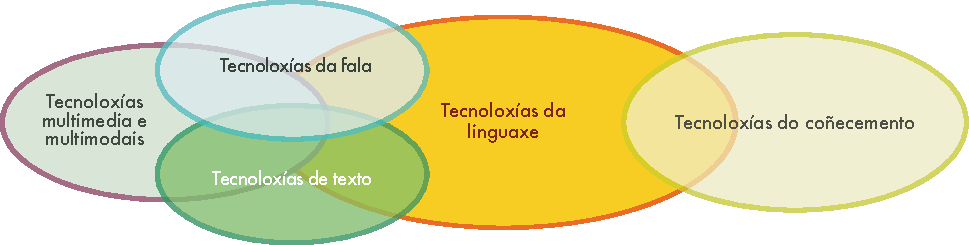
\includegraphics[width=\textwidth]{../_media/galician/language_technologies}
  \caption{Tecnoloxías da linguaxe}
  \label{fig:ltincontext_ga}
  \colorrule{grey3}{\textwidth}{1.5pt}
\end{figure*}

A tecnoloxía da lingua é unha área establecida de investigación cun conxunto extenso de bibliografía introdutoria. O lector que estea interesado pode consultar ás referencias seguintes: \cite{carstensen-etal1,jurafsky-martin01, manning-schuetze1, lt-world1, lt-survey1}.

Antes de discutir sobre as áreas de aplicación citadas, imos describir brevemente a arquitectura dun sistema de tecnoloxía da lingua típico.

\subsection[As arquitecturas das aplicacións na tecnoloxías lingüísticas]{As arquitecturas das \newline aplicacións na tecnoloxías lingüísticas}

    As aplicacións informáticas habituais para o tratamento da linguaxe consisten en varios compoñentes que reflicten diversos aspectos da linguaxe e da tarefa que levan a cabo. A Figura~\ref{fig:textprocessingarch_ga} presenta unha arquitectura moi simplificada que pode atoparse nun sistema de procesamento de textos. Os tres primeiros módulos tratan a estrutura e o significado do texto de entrada:

\begin{itemize}
      \item Procesamento previo: limpar os datos, eliminar formato, detectar a lingua do texto de entrada, etc.
      \item Análise gramatical: atopar o verbo e os seus obxectos, modificadores, etc.; detectar a estrutura da oración.
      \item Análise semántica: desambiguación (cal dos significados de \textit{gato} é o axeitado no contexto dado?), resolución de anáforas e expresións referenciais como \textit{ela}, o \textit{coche}, etc.; representación do significado da oración de xeito que se poida facer unha lectura automática.
\end{itemize}

\begin{figure*}[b]
  \colorrule{grey3}{\textwidth}{1.5pt}
  \center
  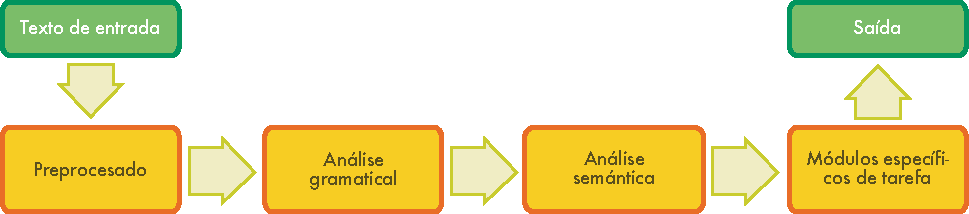
\includegraphics[width=\textwidth]{../_media/galician/text_processing_app_architecture}
  \caption{Arquitectura típica dunha aplicación de procesamento de texto}
  \label{fig:textprocessingarch_ga}
  \colorrule{grey3}{\textwidth}{1.5pt}
\end{figure*}

    Os módulos de tarefas específicas levan a cabo diferentes operacións, tales como o resumo automático dun texto de entrada, consultas de bases de datos, e moitas outras. Abaixo, mostraremos as áreas principais de aplicación e destacaremos os seus módulos principais. Novamente, as arquitecturas das aplicacións aparecen moi simplificadas para mostrar a complexidade das aplicacións da tecnoloxía lingüística (TL) dun xeito comprensible para o público xeral. 

Tras facer unha introdución sobre as áreas principais de aplicación, faremos un pequeno repaso da situación na investigación aplicada á tecnoloxía lingüística e á educación, concluíndo cun resumo dos programas de investigación pasados e actuais. Ao final desta sección ofreceremos a opinión dos expertos sobre a situación das principais ferramentas e recursos da tecnoloxía lingüística no tocante a varios aspectos, como a súa dispoñibilidade, madurez ou calidade. Unha visión de conxunto sobre a situación da TL para o galego atópase na táboa~\ref{fig:lrlttable_ga} (p.~\pageref{fig:lrlttable_ga}) ao final do capítulo. Esta táboa lista as ferramentas e recursos que aparecen \textbf{en negriña} no texto.
%As seccións que tratan das principais áreas de aplicación tamén conteñen un resumo do mercado activo nos campos respectivos para o galego. 
% CGM: done
%FIXME please change this accordingly

\subsection{Principais áreas de aplicación} 

%As ferramentas e recursos máis importantes aparecen \textbf{en negriña} e tamén se poden atopar na táboa \ref{fig:lrlttable_ga} ao final do capítulo (p. \ref{fig:lrlttable_ga}).
As seccións que tratan das principais áreas de aplicación tamén conteñen un resumo do mercado activo nos campos respectivos para o galego. 

\subsubsection{A corrección lingüística}

\begin{figure*}[htb]
  \colorrule{grey3}{\textwidth}{1.5pt}
  \center
  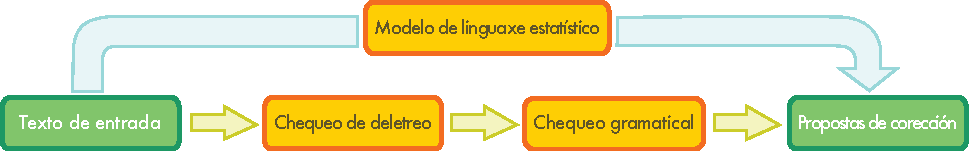
\includegraphics[width=\textwidth]{../_media/galician/language_checking}
  \caption{Comprobación de linguaxe (parte superior: estatística, inferior: baseada en regras)}
  \label{fig:langcheckingaarch_ga}
  \colorrule{grey3}{\textwidth}{1.5pt}
\end{figure*}

Calquera persoa que empregue unha ferramenta de procesamento de textos, como Microsoft Word, atoparase coa opción de corrección ortográfica, que indica os erros de ortografía e propón as súas correccións. Corenta anos despois do primeiro programa de corrección ortográfica deseñado por Ralph Gorin, hoxe en día os correctores lingüísticos non só comparan a lista de palabras extraídas cun dicionario de palabras correctamente escritas, senón que estes son cada vez máis sofisticados. Ademais dos algoritmos d'\textbf{análise gramatical} que dependen do idioma para o tratamento da morfoloxía (por exemplo, a formación do plural), algúns son agora capaces de recoñecer erros relacionados coa sintaxe, tales como a omisión do verbo ou un verbo que non estea acorde co seu suxeito en persoa e número (por exemplo, “Ela *\underline{escriben} unha carta”). Non obstante, para outros tipos de erros comúns, os métodos anteriormente descritos non son suficientes. Por exemplo, botémoslle unha ollada a continuación ao primeiro verso dun poema escrito por Jerrold H.~Zar (1992): 

\begin{verse}
\textit{Eye have a spelling chequer,} \\
\textit{It came with my Pea Sea.} \\
\textit{It plane lee marks four my revue} \\
\textit{Miss Steaks I can knot sea.} 
\end{verse}

A meirande parte dos correctores ortográficos (incluído Microsoft Word) non atoparán erros neste poema, porque se fixan principalmente nas palabras de forma illada. Non obstante, para detectar os erros chamados homófonos (por exemplo, “Eye" no canto de “I"), o corrector lingüístico ten que considerar o contexto no que se atopa a palabra. No caso do galego, mesmo a corrección ortográfica require unha análise do contexto en moitos casos. Un caso típico sucede cando o erro ortográfico transforma unha palabra noutra que tamén existe. No seguinte exemplo, a primeira frase contén un erro frecuente (problemas con acentos ortográficos). A segunda frase é a versión corrixida da primeira.

\begin{itemize}
\item[]\textit{A casa do meu tío \textbf{e} a casa da miña avoa.}
\item[]\textit{A casa do meu tío \textbf{é} a casa da miña avoa.} 
\end{itemize}
 
Para corrixir automaticamente estes erros, non é suficiente facer unha comprobación de cada palabra no dicionario, xa que todas as palabras da primeira frase son correctas de forma illada. Isto ou ben require a formulación de \textbf{gramáticas} específicas para cada lingua (é dicir, un alto grao de experiencia e traballo manual), ou o uso dun modelo lingüístico estatístico. Estes modelos calculan a probabilidade de que se dea unha palabra nun contexto específico (é dicir, as palabras anteriores e as seguintes). Por exemplo, “é a" é unha secuencia de palabras moito máis probable que “e a". Ao empregar unha grande cantidade de datos (correctos) lingüísticos (é dicir, un \textbf{corpus textual}), pódese obter automaticamente un modelo lingüístico estatístico. Ata o de agora, este tipo de mecanismos foron principalmente desenvolvidos e avaliados con datos do idioma inglés. Non obstante, non sempre son aplicables a outras linguas, como por exemplo as linguas sintéticas ou as linguas con flexión sintáctica, como o galego. Para estes idiomas máis complexos, un corrector lingüístico avanzado de alta precisión requirirá o desenvolvemento de métodos máis sofisticados e que implican unha análise lingüística máis profunda.

\boxtext{Os correctores lingüísticos son cada vez máis sofisticados.}

O emprego dos correctores lingüísticos non está limitado ás ferramentas de procesamento de textos, senón que tamén se aplican no \textit{software} de autoría. Xunto co aumento de produtos técnicos, durante as últimas décadas tamén se incrementou a cantidade de documentación técnica. Por temor a recibir reclamacións de clientes por danos e prexuízos como resultado dunhas malas instrucións, ou da súa mala comprensión, as compañías comezaron a centrarse cada vez máis na calidade da documentación técnica, coa intención, ao mesmo tempo, de chegar ao mercado internacional. Os avances no procesamento da linguaxe natural levaron ao desenvolvemento de \textit{software} de autoría, que axuda ao redactor da documentación técnica a empregar vocabulario e estruturas sintácticas coherentes seguindo certas normas e restricións terminolóxicas (corporativas). 

\boxtext{A revisión da linguaxe non só se limita aos procesadores de texto  senón que tamén se aplica a ferramentas de autor.}


Só unhas poucas empresas e provedores de servizos lingüísticos ofrecen produtos nesta área para o galego. O software \textit{Imaxin} \cite{GAL-Nota21} é un exemplo, xa que ofrece servizos en liña gratuítos de tradución e corrección gramatical. O software \textit{OrtoGal}, do Seminario de Lingüística Informática (SLI) \cite{GAL-Nota22} da Universidade de Vigo, ofrece un servizo de corrección gramatical e ortográfica. Tamén existen extensións de software para OpenOffice, como \textit{Golfiño} \cite{GAL-Nota23}, creado por \textit{Imaxin Software} e promovido pola Xunta de Galicia.

Ademais dos correctores ortográficos e do \textit{software} de autoría, a corrección lingüística tamén é importante no eido da aprendizaxe de linguas asistida por ordenador, así coma nos motores de busca na web, onde se aplica para corrixir automaticamente as consultas realizadas, como as suxestións de Google “Quizais quixo dicir\dots". 


\subsubsection{A busca na web}

\begin{figure*}[htb]
  \colorrule{grey3}{\textwidth}{1.5pt}
  \center
  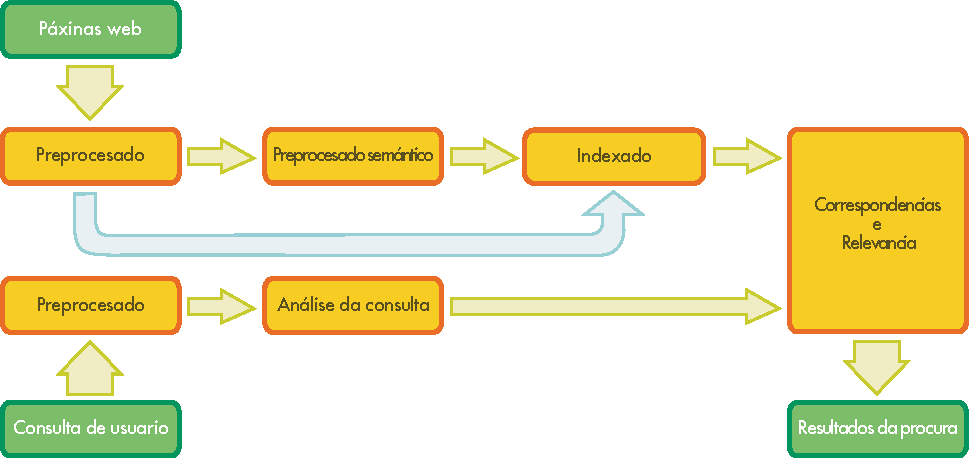
\includegraphics[width=\textwidth]{../_media/galician/web_search_architecture}
  \caption{Buscador web}
  \label{fig:websearcharch_ga}
  \colorrule{grey3}{\textwidth}{1.5pt}
\end{figure*}

A busca na web, en intranets, ou en bibliotecas dixitais é probablemente a tecnoloxía lingüística máis empregada hoxe en día á vez que é a menos desenvolvida. O motor de busca Google, que se creou no ano 1998, emprégase hoxe en día para o 80\% das buscas que se realizan en todo o mundo \cite{googleleavesbehind}.

Ata o de agora, non houbo cambios significativos con respecto á primeira versión no referente á súa interface de busca nin ao xeito de presentar os resultados obtidos. Na versión actual, Google ofrece unha corrección gramatical para as palabras escritas incorrectamente, mesmo para a versión en galego, e, no ano 2009, incorporáronse posibilidades de busca semántica básica ao seu conxunto de algoritmos \cite{googlesemanticsearch}, que melloran a precisión da busca mediante unha análise do significado dos termos da consulta dentro dun contexto. O caso do éxito de Google demostra que, dispoñendo dunha grande cantidade de datos, e con técnicas eficientes para a indexación destes datos, un método baseado principalmente en estatísticas pode producir resultados satisfactorios. 

Non obstante, cando hai unha solicitude de información máis complexa, é fundamental integrar un coñecemento lingüístico máis profundo. Nos laboratorios de investigación, os experimentos levados a cabo empregando \textbf{recursos léxicos} como tesouros e recursos lingüísticos ontolóxicos como \textit{WordNet} amosaron melloras ao permitir a posibilidade de atopar unha páxina baseándose en sinónimos dos termos empregados na busca, ou mesmo en termos non relacionados directamente. Novamente, estes avances esixen uns recursos lingüísticos específicos. O Centro Ramón Piñeiro para a Investigación en Humanidades \cite{GAL-Nota24} elaborou un \textit{WordNet} para o galego. O \textit{WordNet} galego chámase GALWORDNET.

A próxima xeración de motores de busca terá que incluír unha tecnoloxía lingüística moito máis sofisticada. Se unha busca consiste nunha pregunta, ou noutro tipo de frase que non se trate dunha listaxe de palabras clave, é precisa unha \textbf{análise semántico} e sintáctico desta frase, así como a dispoñibilidade dun índice que permita unha rápida recuperación de documentos relevantes, para poder obter respostas relevantes. Por exemplo, imaxinemos que o usuario introduce a busca: “Dáme unha lista de todas as compañías que foron absorbidas por outras compañías nos últimos cinco anos". Para obter un resultado satisfactorio, é necesario realizar unha análise sintáctica para analizar a estrutura gramatical da frase e determinar que o usuario está buscando compañías que foron absorbidas, e non compañías que absorberon outras compañías. Así mesmo, a expresión “últimos cinco anos" tamén ten que ser procesada para saber a que anos se refire. 

Finalmente, a solicitude procesada contrástase cunha grande cantidade de datos non estruturados para atopar a información ou as informacións que o usuario está a solicitar. Este proceso coñécese habitualmente como recuperación da información, e implica a busca e a clasificación de documentos relevantes. Ademais, á hora de xerar un listado de compañías, tamén necesitamos extraer a información que fai referencia ao nome dunha compañía dentro dunha cadea de palabras concreta situada nun documento. Este tipo de información está dispoñible grazas aos chamados recoñecedores de nomes de entidades. 

Unha tarefa aínda máis difícil é intentar facer coincidir unha busca con documentos escritos noutro idioma. Para a recuperación de información plurilingüe, temos que traducir automaticamente a consulta a todas as posibles linguas fonte e volver a pasar a información recuperada á lingua meta. A crecente porcentaxe de datos dispoñibles en formatos non textuais enfoca a demanda cara a servizos que permiten a recuperación de información multimedia (é dicir, a busca de información en imaxes, audio e vídeo). Para os arquivos de audio e vídeo, introdúcese un módulo de recoñecemento do discurso, que converte o contido do discurso en texto ou nunha representación fonética, e pode facer coincidir coa consulta realizada polo usuario.

\boxtext{A seguinte xeración de motores de busca terá que incluír tecnoloxía de lingua moito máis sofisticada.}

Non nos consta que exista tecnoloxía lingüística en compañías dedicadas á busca plurilingüe e á recuperación de información, tanto na Internet como en sistemas de información internos, para o galego. 

\subsubsection{A interacción da fala}

A tecnoloxía de interacción da fala é a base para a creación de interfaces que permiten ao usuario interactuar con máquinas empregando a lingua falada no canto de, por exemplo, un teclado, un rato ou unha pantalla gráfica. Hoxe en día, estas interfaces de usuario baseadas en voz empréganas habitualmente as empresas para proporcionar aos seus clientes, empregados, ou socios, servizos parcialmente ou totalmente automatizados por vía telefónica. 

Os sectores empresariais que dependen en gran medida das interfaces de usuario baseadas en voz son: a banca, a loxística, o transporte público e as telecomunicacións. Outros usos da tecnoloxía de interacción da fala son as interfaces de certos aparellos, como os sistemas de navegación integrados nos automóbiles, ou o emprego da lingua falada como alternativa ás modalidades de entrada e saída de información nas interfaces gráficas de usuario, como por exemplo os \textit{smartphones}.


\begin{figure*}[htb]
  \colorrule{grey3}{\textwidth}{1.5pt}
  \center
  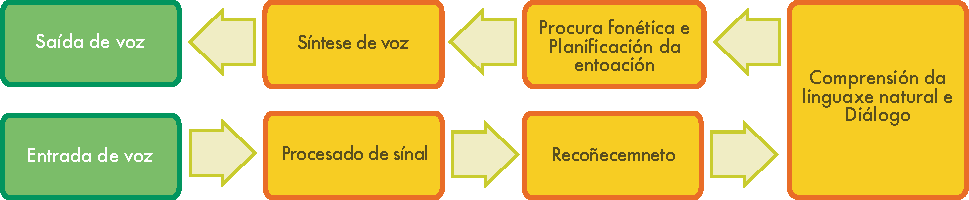
\includegraphics[width=\textwidth]{../_media/galician/simple_speech-based_dialogue_architecture}
%  \center
  \caption{Sistema de diálogo baseado en fala}
  \label{fig:dialoguearch_ga}
  \colorrule{grey3}{\textwidth}{1.5pt}
\end{figure*}

En esencia, a interacción da fala consta das seguintes catro tecnoloxías: 

\begin{itemize}
      \item O \textbf{recoñecemento automático da fala } (RAF) é o responsable de determinar que palabras foron emitidas tendo en conta a secuencia de sons pronunciados por un usuario.
      \item A \textbf{análise sintáctica } e a interpretación semántica ocúpanse de analizar a estrutura sintáctica da locución do usuario e da súa posterior interpretación en función da finalidade do sistema respectivo.
      \item A xestión do diálogo é necesaria para determinar, pola parte do sistema coa que interactúa o usuario, que acción debe levarse a cabo tendo en conta o \textit{input} do usuario e a funcionalidade do sistema.
      \item A tecnoloxía de  \textbf{síntese da fala} (texto a voz, TAV) emprégase para transformar as palabras que se emitiron nesa locución en sons que xerarán como resultado unha información de saída para o usuario.  
\end{itemize}

Un dos maiores retos é que o sistema de RAF recoñeza as palabras pronunciadas por un usuario do xeito máis preciso posible. Isto require ou ben unha restrición da variedade de posibles pronuncias do usuario, para así contar cun conxunto limitado de palabras clave, ou a creación manual de modelos de linguaxe que cubran unha grande variedade de pronuncias de usuarios da linguaxe natural. Mentres que o anterior dá como resultado un uso bastante ríxido e inflexible dunha interface de usuario baseada en voz, e posiblemente provoque unha mala aceptación por parte do usuario, a creación, optimización e mantemento de modelos de linguaxe chegan a aumentar os custos considerablemente. Non obstante, as interfaces de usuario baseadas en voz que empregan modelos de linguaxe e que inicialmente permiten que o usuario exprese con flexibilidade as súas intencións (como, por exemplo, nun saúdo como “En que podo axudarlle") amosan tanto un maior grao de automatización como unha maior aceptación por parte do usuario e, polo tanto, poden considerarse vantaxosas mesmo cun enfoque de \textit{diálogo dirixido }  menos flexible.

\boxtext{Interacción por voz é a base para interfaces que lle permiten a un usuario interactuar mediante fala.}

No que respecta á saída de información das interfaces de usuario baseadas en voz, as empresan a miúdo adoitan empregar fórmulas previamente gravadas por locutores profesionais (a ser posibles corporativos). Para as locucións estáticas, nas que a redacción non depende do contexto particular de uso, ou dos datos persoais do usuario determinado, isto dará lugar a unha experiencia de usuario satisfactoria. Non obstante, canto máis dinámico sexa o contido que a locución deba ter en conta, a experiencia de usuario sufrirá máis dunha mala prosodia como resultado da concatenación de arquivos de audio individuais. Pola contra, os sistemas actuais de texto a voz demostran ser superiores, a pesar de que se poden mellorar, no referente á naturalidade prosódica das locucións dinámicas. 

Con respecto ao mercado das tecnoloxías de interacción da fala, a última década caracterizouse por unha forte estandarización das interfaces entre os diferentes compoñentes tecnolóxicos, así como polas normas para a creación de aparatos de software particulares para unha determinada aplicación. Tamén existiu unha forte consolidación de mercado nos últimos dez anos, especialmente nos campos do RAF e o TAV. Neste caso, os mercados nacionais dos países do G20 (é dicir, países economicamente fortes cunha poboación considerable) están dominados por menos de 5 reprodutores en todo o mundo, dos cales \textit{Nuance e Loquendo} destacan en Europa, así como para o galego (\textit{Loqueando}); non obstante, algunhas compañías locais máis pequenas están comezando a facer competencia, tales como Verbio \cite{GAL-Nota25} , que é unha versión da Universitat Politècnica de Catalunya e que ten a súa propia tecnoloxía da fala, ou a galega 2Mares \cite{GAL-Nota26}.

En relación á tecnoloxía e ás destrezas de coñecemento da xestión do diálogo, os mercados están fortemente dominados por reprodutores nacionais, que a miúdo se tratan de PEMEs.
A maioría das compañías no mercado do TAV español (algunhas ofrecen galego) son fundamentalmente desenvolvedoras de aplicacións. Os principais reprodutores no mercado español son: Indsys \cite{GAL-Nota27} (Sistemas de diálogo intelixente), Fonetic \cite{GAL-Nota28}, Ydilo \cite{GAL-Nota29}, NaturalVoz \cite{GAL-Nota30}, e 2Mares.

Pero máis aló do estado actual da tecnoloxía, xurdirán importantes cambios debido ao hábito, cada vez máis profuso, de empregar os teléfonos intelixentes (\textit{smartphones}) como unha nova plataforma para xestionar as relacións cos clientes (ademais doutros canais como o teléfono, Internet e o correo electrónico). Esta tendencia tamén afectará ao uso da tecnoloxía para a interacción da fala. Por unha banda, diminuirá a largo prazo a demanda de interfaces de usuario baseadas en telefonía. Por outra banda, o emprego da lingua falada cobrará unha importancia considerable nos \textit{smartphones} como modalidade de entrada de información fácil de empregar polos usuarios. Esta tendencia tamén está reforzada pola mellora perceptible de precisión no recoñecemento independente da voz do locutor nos servizos de ditado de discurso que xa se ofrecen como servizos centralizados para os usuarios de \textit{smartphones}. Dada esta “externalización" da tarefa de recoñecemento á infraestrutura das aplicacións, o emprego específico nas aplicacións de tecnoloxías lingüísticas básicas adquirirá probablemente máis importancia que na actualidade. 

\subsubsection{A tradución automática}

  A idea de empregar ordenadores dixitais para a tradución de linguas naturais foi desenvolvida no ano 1946 por A.~D.~Booth e, na década dos 50, foi acompañada dun financiamento importante para a investigación nesta área, que comezou novamente na década dos 80. Non obstante, a \textbf{Tradución Automática} (TA) aínda non consigue cumprir as grandes expectativas que se esperaban nos seus inicios. 

\boxtext{No seu nivel básico, a tradución automática simplemente fai a substitución de palabras dunha lingua por palabras doutra lingua.}

\begin{figure*}[htb]
  \colorrule{grey3}{\textwidth}{1.5pt}
  \center
  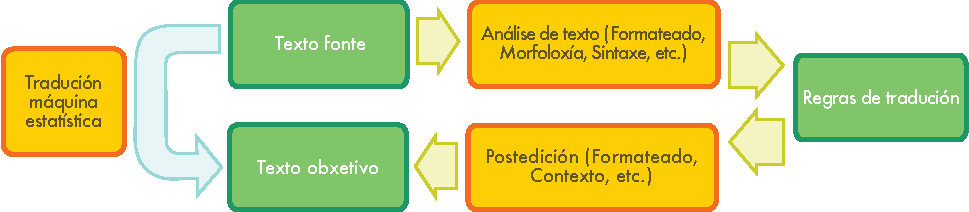
\includegraphics[width=\textwidth]{../_media/galician/machine_translation}
  \caption{Tradución automática (esquerda: estatística, dereita: baseada en regras)}
  \label{fig:mtarch_ga}
  \colorrule{grey3}{\textwidth}{1.5pt}
\end{figure*}

No seu nivel básico, a TA simplemente substitúe palabras nunha lingua natural por palabras noutra. Isto pode resultar útil en disciplinas que posúen unha linguaxe moi restrinxida e con fórmulas establecidas, tales como os informes meteorolóxicos. Non obstante, para que exista unha boa tradución dos textos menos estandarizados, as unidades textuais máis grandes (frases, oracións, ou mesmo pasaxes completas) teñen que coincidir coas súas unidades homólogas máis próximas na lingua meta. Neste caso, a principal dificultade reside no feito de que a linguaxe humana é ambigua, e presenta retos a varios niveis, como por exemplo a \textbf{desambiguación do sentido da palabra} a nivel léxico (“Gato" pode significar animal ou aparello mecánico), ou a vinculación de frases preposicionais a nivel sintáctico como en:

\begin{itemize}
\item[] \textit{O policía observou ao home co telescopio}
%\hspace{10pt}\textit{[The policeman observed the man with the telescope.]}\\
\item[]\textit{O policía observou ao home co revólver.}
%\hspace{10pt}\textit{[The policeman observed the man with the revolver.]}
\end{itemize}

Unha das maneiras para abordar esta tarefa está baseada en regras lingüísticas. Para traducións entre linguas moi relacionadas, unha tradución directa pode resultar viable en casos como o exemplo presentado anteriormente. Non obstante, a miúdo os sistemas baseados en regras (ou baseados no coñecemento) analizan o texto de entrada e crean unha representación simbólica intermediaria, a partir da cal se crea o texto na lingua meta. O éxito destes métodos depende en boa medida da dispoñibilidade de \textbf{lexicóns} extensos que contan con información morfolóxica, sintáctica e semántica, así como de grandes conxuntos de regras \textbf{gramaticais} coidadosamente deseñadas por lingüistas especializados.

Comezando a finais da década de 1980, e nunha situación na que a informática ía avanzando e se volvía menos cara, empezou a mostrarse cada máis interese nos modelos estatísticos de TA. Os parámetros destes modelos estatísticos derívanse da análise de \textbf{corpus paralelos} textuais bilingües, como o corpus paralelo Europarl, que contén as actas do Parlamento Europeo en 21 linguas europeas. Cunha cantidade de datos suficiente, a TA estatística funciona bastante ben á hora de obter un significado aproximado dun texto nunha lingua estranxeira. Non obstante, a diferenza dos sistemas baseados no coñecemento, a TA estatística (ou baseada en bases de datos) a miúdo obtén un resultado gramaticalmente incorrecto. Por outra banda, ademais de que grazas a ela requírese menos esforzo humano para realizar unha escritura gramaticalmente correcta, a TA baseada en datos tamén inclúe particularidades da linguaxe que non se inclúen nos sistemas baseados no coñecemento, como por exemplo as expresións idiomáticas. 

Xa que os puntos fortes e febles da TA baseada no coñecemento e da TA baseada en datos son complementarios, hoxe en día os investigadores buscan enfoques híbridos que combinen as metodoloxías de ambas as dúas. Isto pode levarse a cabo de diferentes maneiras. Unha delas é empregar tanto os sistemas baseados en coñecemento como os sistemas baseados en datos e facer que un módulo de selección elixa o mellor resultado para cada oración. Non obstante, no caso das oracións máis longas, non existe un resultado perfecto. Unha solución mellor sería combinar as mellores partes de cada oración extraídas de múltiples resultados, o cal pode resultar bastante complexo, xa que as partes correspondentes obtidas de múltiples alternativas non sempre son obvias e necesitan ser aliñadas. 

O desenvolvedor de software líder a nivel internacional Lucy Software ten unha importante filial en España, Lucy Iberica \cite{GAL-Nota31}, anteriormente coñecida como Translendium. Lucy Ibérica encárgase do desenvolvemento de pares de linguas que inclúen o español, así como de todos os pares de linguas que implican calquera outra lingua ibérica (catalán, portugués, galego e éuscaro). O sistema de Lucy está baseado en regras gramaticais. A Xunta de Galicia \cite{GAL-Nota32} ofrece un servizo de tradución na Internet que emprega a tecnoloxía de Lucy Iberica. A pesar das importantes investigacións levadas a cabo sobre os sistemas baseados en datos e os sistemas híbridos a nivel nacional e internacional, ata o de agora esta tecnoloxía tivo menos éxito no eido comercial que no eido da investigación.

Apertium é unha plataforma de tradución automática libre que proporciona un motor de tradución automática independentemente da lingua da que se trate. Esta plataforma foi deseñada polo grupo Transducens da Universitat d'Alacant, e posteriormente desenvolvida no marco do proxecto de financiamento nacional Opentrad. Entre os actuais \textbf{sistemas} de TA que empregan a tecnoloxía Apertium atopamos interNOSTRUM (español-catalán), desenvolvido por Transducens, o Traductor Universia (español-portugués), Matxin (éuscaro-español), desenvolvido polo grupo IXA \cite{GAL-Nota33} da Euskal Herriko Unibertsitatea, e Imaxin Software (galego-español). É posible empregar a tecnoloxía Apertium para construír sistemas de TA para unha variedade de pares de linguas (existen máis de 20 ata a data); con ese fin, Apertium emprega formatos estándar baseados en XML para codificar os datos lingüísticos necesarios (facéndoo a man ou convertendo os datos existentes) que se compilan, empregando as ferramentas proporcionadas, nos formatos de alta velocidade que emprega o motor. 

En tanto exista unha boa adaptación no referente á terminoloxía específica do usuario e unha integración do fluxo de traballo, hai un amplo consenso á hora de establecer que o uso da TA pode aumentar a produtividade de maneira significativa. 

Así e todo, considérase que a calidade dos sistemas de TA aínda ten un grande potencial de mellora. Entre os retos de mellora que se presentan, cabe citar a adaptabilidade dos recursos lingüísticos a unha disciplina específica ou área do usuario, e a integración dentro de fluxos de traballo existentes con bases terminolóxicas e memorias de tradución. Ademais disto, aínda faltan moitos pares de linguas. 


\begin{figure*}[htb]
  \centering
  \setlength{\tabcolsep}{0.17em}
  \small
  \begin{tabular}{>{\columncolor{corange1}}cccccccccccccccccccccccc}
    & \multicolumn{22}{>{\columncolor{corange1}}c}{Lingua obxectivo  --- \textcolor{grey1}{Target language}}\\\addlinespace[{-.009cm}]
    \rowcolor{corange1}  & EN & BG & DE & CS & DA & EL & ES & ET & FI & FR & HU & IT & LT & LV & MT & NL & PL & PT & RO & SK & SL & SV\\
    EN & -- & \textcolor{blue}{40.5} & \textcolor{blue}{46.8} & \textcolor{green2}{52.6} & \textcolor{green2}{50.0} & \textcolor{blue}{41.0} & \textcolor{green2}{55.2} & \textcolor{purple}{34.8} & \textcolor{purple}{38.6} & \textcolor{green2}{50.1} & \textcolor{purple}{37.2} & \textcolor{green2}{50.4} & \textcolor{purple}{39.6} & \textcolor{blue}{43.4} & \textcolor{purple}{39.8} & \textcolor{green2}{52.3} & \textcolor{blue}{49.2} & \textcolor{green2}{55.0} & \textcolor{blue}{49.0} & \textcolor{blue}{44.7} & \textcolor{green2}{50.7} & \textcolor{green2}{52.0}\\
    BG & \textcolor{green}{61.3} & -- & \textcolor{purple}{38.7} & \textcolor{purple}{39.4} & \textcolor{purple}{39.6} & \textcolor{purple}{34.5} & \textcolor{blue}{46.9} & \textcolor{red3}{25.5} & \textcolor{red3}{26.7} & \textcolor{blue}{42.4} & \textcolor{red3}{22.0} & \textcolor{blue}{43.5} & \textcolor{red3}{29.3} & \textcolor{red3}{29.1} & \textcolor{red3}{25.9} & \textcolor{blue}{44.9} & \textcolor{purple}{35.1} & \textcolor{blue}{45.9} & \textcolor{purple}{36.8} & \textcolor{purple}{34.1} & \textcolor{purple}{34.1} & \textcolor{purple}{39.9}\\
    DE & \textcolor{green2}{53.6} & \textcolor{red3}{26.3} & -- & \textcolor{purple}{35.4} & \textcolor{blue}{43.1} & \textcolor{purple}{32.8} & \textcolor{blue}{47.1} & \textcolor{red3}{26.7} & \textcolor{red3}{29.5} & \textcolor{purple}{39.4} & \textcolor{red3}{27.6} & \textcolor{blue}{42.7} & \textcolor{red3}{27.6} & \textcolor{purple}{30.3} & \textcolor{red2}{19.8} & \textcolor{green2}{50.2} & \textcolor{purple}{30.2} & \textcolor{blue}{44.1} & \textcolor{purple}{30.7} & \textcolor{red3}{29.4} & \textcolor{purple}{31.4} & \textcolor{blue}{41.2}\\
    CS & \textcolor{green2}{58.4} & \textcolor{purple}{32.0} & \textcolor{blue}{42.6} & -- & \textcolor{blue}{43.6} & \textcolor{purple}{34.6} & \textcolor{blue}{48.9} & \textcolor{purple}{30.7} & \textcolor{purple}{30.5} & \textcolor{blue}{41.6} & \textcolor{red3}{27.4} & \textcolor{blue}{44.3} & \textcolor{purple}{34.5} & \textcolor{purple}{35.8} & \textcolor{red3}{26.3} & \textcolor{blue}{46.5} & \textcolor{purple}{39.2} & \textcolor{blue}{45.7} & \textcolor{purple}{36.5} & \textcolor{blue}{43.6} & \textcolor{blue}{41.3} & \textcolor{blue}{42.9}\\
    DA & \textcolor{green2}{57.6} & \textcolor{red3}{28.7} & \textcolor{blue}{44.1} & \textcolor{purple}{35.7} & -- & \textcolor{purple}{34.3} & \textcolor{blue}{47.5} & \textcolor{red3}{27.8} & \textcolor{purple}{31.6} & \textcolor{blue}{41.3} & \textcolor{red3}{24.2} & \textcolor{blue}{43.8} & \textcolor{red3}{29.7} & \textcolor{purple}{32.9} & \textcolor{red3}{21.1} & \textcolor{blue}{48.5} & \textcolor{purple}{34.3} & \textcolor{blue}{45.4} & \textcolor{purple}{33.9} & \textcolor{purple}{33.0} & \textcolor{purple}{36.2} & \textcolor{blue}{47.2}\\
    EL & \textcolor{green2}{59.5} & \textcolor{purple}{32.4} & \textcolor{blue}{43.1} & \textcolor{purple}{37.7} & \textcolor{blue}{44.5} & -- & \textcolor{green2}{54.0} & \textcolor{red3}{26.5} & \textcolor{red3}{29.0} & \textcolor{blue}{48.3} & \textcolor{red3}{23.7} & \textcolor{blue}{49.6} & \textcolor{red3}{29.0} & \textcolor{purple}{32.6} & \textcolor{red3}{23.8} & \textcolor{blue}{48.9} & \textcolor{purple}{34.2} & \textcolor{green2}{52.5} & \textcolor{purple}{37.2} & \textcolor{purple}{33.1} & \textcolor{purple}{36.3} & \textcolor{blue}{43.3}\\
    ES & \textcolor{green}{60.0} & \textcolor{purple}{31.1} & \textcolor{blue}{42.7} & \textcolor{purple}{37.5} & \textcolor{blue}{44.4} & \textcolor{purple}{39.4} & -- & \textcolor{red3}{25.4} & \textcolor{red3}{28.5} & \textcolor{green2}{51.3} & \textcolor{red3}{24.0} & \textcolor{green2}{51.7} & \textcolor{red3}{26.8} & \textcolor{purple}{30.5} & \textcolor{red3}{24.6} & \textcolor{blue}{48.8} & \textcolor{purple}{33.9} & \textcolor{green2}{57.3} & \textcolor{purple}{38.1} & \textcolor{purple}{31.7} & \textcolor{purple}{33.9} & \textcolor{blue}{43.7}\\
    ET & \textcolor{green2}{52.0} & \textcolor{red3}{24.6} & \textcolor{purple}{37.3} & \textcolor{purple}{35.2} & \textcolor{purple}{37.8} & \textcolor{red3}{28.2} & \textcolor{blue}{40.4} & -- & \textcolor{purple}{37.7} & \textcolor{purple}{33.4} & \textcolor{purple}{30.9} & \textcolor{purple}{37.0} & \textcolor{purple}{35.0} & \textcolor{purple}{36.9} & \textcolor{red3}{20.5} & \textcolor{blue}{41.3} & \textcolor{purple}{32.0} & \textcolor{purple}{37.8} & \textcolor{red3}{28.0} & \textcolor{purple}{30.6} & \textcolor{purple}{32.9} & \textcolor{purple}{37.3}\\
    FI & \textcolor{blue}{49.3} & \textcolor{red3}{23.2} & \textcolor{purple}{36.0} & \textcolor{purple}{32.0} & \textcolor{purple}{37.9} & \textcolor{red3}{27.2} & \textcolor{purple}{39.7} & \textcolor{purple}{34.9} & -- & \textcolor{red3}{29.5} & \textcolor{red3}{27.2} & \textcolor{purple}{36.6} & \textcolor{purple}{30.5} & \textcolor{purple}{32.5} & \textcolor{red2}{19.4} & \textcolor{blue}{40.6} & \textcolor{red3}{28.8} & \textcolor{purple}{37.5} & \textcolor{red3}{26.5} & \textcolor{red3}{27.3} & \textcolor{red3}{28.2} & \textcolor{purple}{37.6}\\
    FR & \textcolor{green}{64.0} & \textcolor{purple}{34.5} & \textcolor{blue}{45.1} & \textcolor{purple}{39.5} & \textcolor{blue}{47.4} & \textcolor{blue}{42.8} & \textcolor{green}{60.9} & \textcolor{red3}{26.7} & \textcolor{purple}{30.0} & -- & \textcolor{red3}{25.5} & \textcolor{green2}{56.1} & \textcolor{red3}{28.3} & \textcolor{purple}{31.9} & \textcolor{red3}{25.3} & \textcolor{green2}{51.6} & \textcolor{purple}{35.7} & \textcolor{green}{61.0} & \textcolor{blue}{43.8} & \textcolor{purple}{33.1} & \textcolor{purple}{35.6} & \textcolor{blue}{45.8}\\
    HU & \textcolor{blue}{48.0} & \textcolor{red3}{24.7} & \textcolor{purple}{34.3} & \textcolor{purple}{30.0} & \textcolor{purple}{33.0} & \textcolor{red3}{25.5} & \textcolor{purple}{34.1} & \textcolor{red3}{29.6} & \textcolor{red3}{29.4} & \textcolor{purple}{30.7} & -- & \textcolor{purple}{33.5} & \textcolor{red3}{29.6} & \textcolor{purple}{31.9} & \textcolor{red2}{18.1} & \textcolor{purple}{36.1} & \textcolor{red3}{29.8} & \textcolor{purple}{34.2} & \textcolor{red3}{25.7} & \textcolor{red3}{25.6} & \textcolor{red3}{28.2} & \textcolor{purple}{30.5}\\
    IT & \textcolor{green}{61.0} & \textcolor{purple}{32.1} & \textcolor{blue}{44.3} & \textcolor{purple}{38.9} & \textcolor{blue}{45.8} & \textcolor{blue}{40.6} & \textcolor{red3}{26.9} & \textcolor{red3}{25.0} & \textcolor{red3}{29.7} & \textcolor{green2}{52.7} & \textcolor{red3}{24.2} & -- & \textcolor{red3}{29.4} & \textcolor{purple}{32.6} & \textcolor{red3}{24.6} & \textcolor{green2}{50.5} & \textcolor{purple}{35.2} & \textcolor{green2}{56.5} & \textcolor{purple}{39.3} & \textcolor{purple}{32.5} & \textcolor{purple}{34.7} & \textcolor{blue}{44.3}\\
    LT & \textcolor{green2}{51.8} & \textcolor{red3}{27.6} & \textcolor{purple}{33.9} & \textcolor{purple}{37.0} & \textcolor{purple}{36.8} & \textcolor{red3}{26.5} & \textcolor{red3}{21.1} & \textcolor{purple}{34.2} & \textcolor{purple}{32.0} & \textcolor{purple}{34.4} & \textcolor{red3}{28.5} & \textcolor{purple}{36.8} & -- & \textcolor{blue}{40.1} & \textcolor{red3}{22.2} & \textcolor{purple}{38.1} & \textcolor{purple}{31.6} & \textcolor{purple}{31.6} & \textcolor{red3}{29.3} & \textcolor{purple}{31.8} & \textcolor{purple}{35.3} & \textcolor{purple}{35.3}\\
    LV & \textcolor{green2}{54.0} & \textcolor{red3}{29.1} & \textcolor{purple}{35.0} & \textcolor{purple}{37.8} & \textcolor{purple}{38.5} & \textcolor{red3}{29.7} & \textcolor{red2}{8.0} & \textcolor{purple}{34.2} & \textcolor{purple}{32.4} & \textcolor{purple}{35.6} & \textcolor{red3}{29.3} & \textcolor{purple}{38.9} & \textcolor{purple}{38.4} & -- & \textcolor{red3}{23.3} & \textcolor{blue}{41.5} & \textcolor{purple}{34.4} & \textcolor{purple}{39.6} & \textcolor{purple}{31.0} & \textcolor{purple}{33.3} & \textcolor{purple}{37.1} & \textcolor{purple}{38.0}\\
    MT & \textcolor{green}{72.1} & \textcolor{purple}{32.2} & \textcolor{purple}{37.2} & \textcolor{purple}{37.9} & \textcolor{purple}{38.9} & \textcolor{purple}{33.7} & \textcolor{blue}{48.7} & \textcolor{red3}{26.9} & \textcolor{red3}{25.8} & \textcolor{blue}{42.4} & \textcolor{red3}{22.4} & \textcolor{blue}{43.7} & \textcolor{purple}{30.2} & \textcolor{purple}{33.2} & -- & \textcolor{blue}{44.0} & \textcolor{purple}{37.1} & \textcolor{blue}{45.9} & \textcolor{purple}{38.9} & \textcolor{purple}{35.8} & \textcolor{blue}{40.0} & \textcolor{blue}{41.6}\\
    NL & \textcolor{green2}{56.9} & \textcolor{red3}{29.3} & \textcolor{blue}{46.9} & \textcolor{purple}{37.0} & \textcolor{blue}{45.4} & \textcolor{purple}{35.3} & \textcolor{blue}{49.7} & \textcolor{red3}{27.5} & \textcolor{red3}{29.8} & \textcolor{blue}{43.4} & \textcolor{red3}{25.3} & \textcolor{blue}{44.5} & \textcolor{red3}{28.6} & \textcolor{purple}{31.7} & \textcolor{red3}{22.0} & -- & \textcolor{purple}{32.0} & \textcolor{blue}{47.7} & \textcolor{purple}{33.0} & \textcolor{purple}{30.1} & \textcolor{purple}{34.6} & \textcolor{blue}{43.6}\\
    PL & \textcolor{green}{60.8} & \textcolor{purple}{31.5} & \textcolor{blue}{40.2} & \textcolor{blue}{44.2} & \textcolor{blue}{42.1} & \textcolor{purple}{34.2} & \textcolor{blue}{46.2} & \textcolor{red3}{29.2} & \textcolor{red3}{29.0} & \textcolor{blue}{40.0} & \textcolor{red3}{24.5} & \textcolor{blue}{43.2} & \textcolor{purple}{33.2} & \textcolor{purple}{35.6} & \textcolor{red3}{27.9} & \textcolor{blue}{44.8} & -- & \textcolor{blue}{44.1} & \textcolor{purple}{38.2} & \textcolor{purple}{38.2} & \textcolor{purple}{39.8} & \textcolor{blue}{42.1}\\
    PT & \textcolor{green}{60.7} & \textcolor{purple}{31.4} & \textcolor{blue}{42.9} & \textcolor{purple}{38.4} & \textcolor{blue}{42.8} & \textcolor{blue}{40.2} & \textcolor{green}{60.7} & \textcolor{red3}{26.4} & \textcolor{red3}{29.2} & \textcolor{green2}{53.2} & \textcolor{red3}{23.8} & \textcolor{green2}{52.8} & \textcolor{red3}{28.0} & \textcolor{purple}{31.5} & \textcolor{red3}{24.8} & \textcolor{blue}{49.3} & \textcolor{purple}{34.5} & -- & \textcolor{purple}{39.4} & \textcolor{purple}{32.1} & \textcolor{purple}{34.4} & \textcolor{blue}{43.9}\\
    RO & \textcolor{green}{60.8} & \textcolor{purple}{33.1} & \textcolor{purple}{38.5} & \textcolor{purple}{37.8} & \textcolor{blue}{40.3} & \textcolor{purple}{35.6} & \textcolor{green2}{50.4} & \textcolor{red3}{24.6} & \textcolor{red3}{26.2} & \textcolor{blue}{46.5} & \textcolor{red3}{25.0} & \textcolor{blue}{44.8} & \textcolor{red3}{28.4} & \textcolor{red3}{29.9} & \textcolor{red3}{28.7} & \textcolor{blue}{43.0} & \textcolor{purple}{35.8} & \textcolor{blue}{48.5} & -- & \textcolor{purple}{31.5} & \textcolor{purple}{35.1} & \textcolor{purple}{39.4}\\
    SK & \textcolor{green}{60.8} & \textcolor{purple}{32.6} & \textcolor{purple}{39.4} & \textcolor{blue}{48.1} & \textcolor{blue}{41.0} & \textcolor{purple}{33.3} & \textcolor{blue}{46.2} & \textcolor{red3}{29.8} & \textcolor{red3}{28.4} & \textcolor{purple}{39.4} & \textcolor{red3}{27.4} & \textcolor{blue}{41.8} & \textcolor{purple}{33.8} & \textcolor{purple}{36.7} & \textcolor{red3}{28.5} & \textcolor{blue}{44.4} & \textcolor{purple}{39.0} & \textcolor{blue}{43.3} & \textcolor{purple}{35.3} & -- & \textcolor{blue}{42.6} & \textcolor{blue}{41.8}\\
    SL & \textcolor{green}{61.0} & \textcolor{purple}{33.1} & \textcolor{purple}{37.9} & \textcolor{blue}{43.5} & \textcolor{blue}{42.6} & \textcolor{purple}{34.0} & \textcolor{blue}{47.0} & \textcolor{purple}{31.1} & \textcolor{red3}{28.8} & \textcolor{purple}{38.2} & \textcolor{red3}{25.7} & \textcolor{blue}{42.3} & \textcolor{purple}{34.6} & \textcolor{purple}{37.3} & \textcolor{purple}{30.0} & \textcolor{blue}{45.9} & \textcolor{purple}{38.2} & \textcolor{blue}{44.1} & \textcolor{purple}{35.8} & \textcolor{purple}{38.9} & -- & \textcolor{blue}{42.7}\\
    SV & \textcolor{green2}{58.5} & \textcolor{red3}{26.9} & \textcolor{blue}{41.0} & \textcolor{purple}{35.6} & \textcolor{blue}{46.6} & \textcolor{purple}{33.3} & \textcolor{blue}{46.6} & \textcolor{red3}{27.4} & \textcolor{purple}{30.9} & \textcolor{purple}{38.9} & \textcolor{red3}{22.7} & \textcolor{blue}{42.0} & \textcolor{red3}{28.2} & \textcolor{purple}{31.0} & \textcolor{red3}{23.7} & \textcolor{blue}{45.6} & \textcolor{purple}{32.2} & \textcolor{blue}{44.2} & \textcolor{purple}{32.7} & \textcolor{purple}{31.3} & \textcolor{purple}{33.5} & --\\
    \end{tabular}
  \caption{Tradución automática (máquina) entre 22 linguas da Unión Europea -- \textcolor{grey1}{Machine translation between 22 EU-languages} \cite{euro1}}
  \label{fig:euromatrix_gal}
\end{figure*}


As campañas de avaliación axudan a comparar a calidade de sistemas de tradución automática, as súas aproximacións e o estado dos sistemas para pares de linguas diferentes. Figura~\ref{fig:euromatrix_gal} (p.~\pageref{fig:euromatrix_gal}), que foi preparada durante o proxecto  Euromatrix+, mostra as prestacións entre pares para 22 das 23 linguas de UE (Irlandés non foi comparado). Os resultados  ordénanse segundo a  BLEU acadada, que indica resultados máis altos para mellores traducións \cite{bleu1}. Un tradutor humano normalmente lograría ao redor de 80 puntos. Os mellores resultados (en verde e azul) foron logrados por linguas que se benefician dun esforzo de investigación considerable  dentro de programas coordinados e para os que se dispón de moitos corpus paralelos (por exemplo, inglés, francés, holandés, español e alemán). As linguas con resultados máis pobres amósanse en vermello. A estas linguas ou ben lle faltan esforzos de desenvolvemento, ou presentan estructuras  moi diferentes das outras linguas (por exemplo,  húngaro, maltés, finlandés).


\subsection{Outras áreas de aplicación}

   A creación de aplicacións de tecnoloxía lingüística implica unha serie de subtarefas que non sempre se desenvolven no plano da interacción co usuario, senón que proporcionan importantes prestacións de servizo “baixo a carcasa" do sistema. Polo tanto, estas aplicacións constitúen asuntos importantes de investigación, e chegaron a converterse en subdisciplinas individuais no ámbito académico dentro da Lingüística Informática. 

\textbf{A resposta a preguntas} converteuse nunha área de investigación, para a cal se construíron \textbf{corpus} anotados e se empezaron a levar a cabo competicións científicas. A idea é pasar da busca baseada en palabras clave (para a cal o motor responde cunha colección enteira de documentos potencialmente relevantes) a unha situación na que o usuario realiza unha pregunta concreta e o sistema proporciona unha soa resposta:

\begin{itemize}
\item[] \textit{Pregunta: A que idade puxo Neil Armstrong pé na lúa?}
\item[] \textit{Responder: 38.}
\end{itemize}

Mentres que isto está obviamente relacionado coa área principal da busca na web, hoxe en día a resposta a preguntas é principalmente un termo xenérico para as preguntas de investigación tales como que tipos de preguntas deberían distinguirse e como deberían tratarse, como poden analizarse e compararse un conxunto de documentos que potencialmente conteñen a resposta (ofrecen respostas contraditorias?), e como pode extraerse de xeito fiable unha información específica -a resposta- dun documento, sen ignorar excesivamente o contexto. 

Isto está, á vez, relacionado coa tarefa de \textbf{extracción de información} (EI), unha área que se volveu moi popular e influente na época do "cambio estatístico" na Lingüística Computacional a principios da década dos 90. A EI ten como obxectivo identificar extractos de información específicos dentro dun tipo específico de documentos; un exemplo disto podería ser o descubrimento dos axentes clave na absorción de empresas tal como informan os artigos xornalísticos. Outra hipótese na que se traballou é os informes sobre atentados terroristas, onde o problema reside en estruturar o texto seguindo un modelo que especifique o autor do crime, o obxectivo, a hora e localización do atentado, e os resultados do mesmo. Cubrir modelos sobre dominios específicos é a principal característica da EI, que por esta razón é outro exemplo dunha tecnoloxía "non visible" que constitúe unha área de investigación ben delimitada pero que, a efectos prácticos, necesita estar integrada dentro dun contorno de aplicacións axeitado. 

\boxtext{As aplicacións da tecnoloxía da linguaxe a miúdo proporcionan un servizo con funcionalidades significativas dentro de sistemas de software máis grandes.}

Existen dúas áreas "dubidosas" que ás veces desempeñan o papel de aplicacións independentes, e outras veces a de compoñentes de apoio "baixo a carcasa" do sistema, que son o resumo do texto e a \textbf{xeración de texto}. O resumo, obviamente, refírese á tarefa de converter un texto longo en curto, e ofrécese, por exemplo, como función dentro de MS Word. Funciona en gran medida sobre unha base estatística, identificando primeiro as palabras “importantes" nun texto (é dicir, por exemplo, palabras que son moi frecuentes neste texto, pero notablemente menos frecuentes no uso xeral da lingua) e, a continuación, determinando as oracións que conteñen moitas palabras importantes. Logo, estas oracións márcanse no documento, ou extráense del, e cóllense para compoñer o resumo. Neste caso, que é sen dúbida o máis común, o resumo é igual á extracción da oración: o texto redúcese a un subconxunto das súas oracións. Todos os resumidores comerciais fan uso desta idea. Un enfoque alternativo, ao que se dedicaron algunhas investigacións, é o de sintetizar novas oracións, é dicir, construír un resumo de oracións que non aparecen necesariamente nesa forma no texto orixinal. Isto require unha certa comprensión máis profunda do texto e, polo tanto, resulta moito menos robusto. En definitiva, un xerador de texto na maioría dos casos non é unha aplicación independente senón que está integrado nun contorno de software máis grande, como no sistema de información clínica onde se recollen, almacenan e procesan os datos dos pacientes, e a xeración de informes é só unha de entre moitas funcións.

\boxtext{Para o galego como para a maioría de linguas, a investigación na maioría das tecnoloxías de texto está moito menos desenvolvida que para o inglés.}

No caso do galego, a situación nestas áreas de investigación está moito menos desenvolvida que no caso do inglés, onde, desde a década de 1990, a resposta a preguntas, a extracción de información e a síntese foron obxecto de numerosas competicións, principalmente as organizadas por DARPA/NIST en Estados Unidos. Estas melloraron notablemente a tecnoloxía punta, pero sempre se fixo fincapé no idioma inglés; algunhas competicións engadiron pistas plurilingües, pero nunca se empregou a lingua galega. Como consecuencia, apenas existen corpus anotados ou outros recursos para estas tarefas. Os sistemas de resumo, cando empregan métodos puramente estatísticos, adoitan ser en boa medida independentes da lingua, e polo tanto están dispoñibles algúns prototipos de investigación. Para a xeración de texto, os compoñentes reutilizables tradicionalmente estaban limitados aos módulos de desenvolvemento da superficie (as “gramáticas de xeración"); unha vez máis, atopamos que a maioría do software dispoñible é para o inglés. 

Ademais dos sistemas experimentais desenvolvidos polos grupos de investigación, non existen PEMEs que ofrezan este tipo de servizos. Desde o ano 2000 ata hoxe, o goberno español vén apoiando, dentro do Plan Nacional de Investigación e Tecnoloxía, varios proxectos na área das tecnoloxías da fala plurilingües: TEHAM, AVIVAVOZ, e BUCEADOR. O seu principal propósito era mellorar a calidade do recoñecemento da fala, da tradución da fala e da síntese de texto a voz en todas as linguas oficiais de España: éuscaro, galego, catalán e español.

\subsection{A tecnoloxía lingüística na educación}

   A tecnoloxía lingüística é un eido sumamente interdisciplinario, no que participan expertos lingüistas, informáticos, matemáticos, filósofos, psicolingüistas e neurólogos, entre outros. Como consecuencia, a actual formación básica dun lingüista informático en España debe levarse a cabo no marco dun título en Filoloxía ou Lingüística, que inclúa á Lingüística Informática como materia troncal, ou nas facultades de Informática. Entre as universidades que ofrecen a primeira opción están: A Universitat de Barcelona, a Universitat Pompeu Fabra, a Universitat Oberta de Catalunya e a Universidade de Vigo. Por outra banda, as principais facultades de informática que ofrecen como materia a Lingüística Informática son: A Universidade Politécnica de Madrid, a Universidade Carlos III, a Universidade Autónoma de Madrid, a Universitat d’Alacant, a Universidade Nacional de Educación a Distancia, e a Euskal Herriko Unibertsitatea. Outros casos, como a Universidade Complutense, combina ambos os dous.

Os cursos de posgrao ofrecen unha formación profesional máis específica. Existen varios programas de doutoramento que ofrecen másteres ou materias relacionadas co procesamento da fala e da linguaxe. Algunhas universidades, como a Universidade Politécnica de Cataluña, tamén participan no Máster Europeo en Linguaxe e Fala, avalado pola ELSNET (Rede de Excelencia Europea en Tecnoloxías Lingüísticas). Existen varios másteres en diversas universidades, a nivel nacional ou a nivel europeo; por exemplo, a Universitat Autònoma de Barcelona ofrece o Máster Internacional en Procesamento de Linguaxe Natural e Tecnoloxías Lingüísticas, en colaboración con universidades estranxeiras. Noutros másteres ou cursos de doutoramento tamén se imparten módulos sobre tecnoloxías lingüísticas, especialmente en Tradución (por exemplo, nas universidades Autónoma de Barcelona, Alacante, Castellón, Politécnica de Valencia e Granada).

Existen máis de 30 grupos de investigación en España repartidos nas diferentes universidades, que traballan no recoñecemento da fala, o procesamento de linguaxe natural, a tradución de texto a texto, e a síntese da fala. A Sociedade Española para o Procesamento da Linguaxe Natural (SEPLN) é unha organización sen ánimo de lucro con máis de 300 membros, tanto do ámbito académico como da industria, que foi creada en 1984 co propósito de promover e difundir as actividades relacionadas coa docencia, a investigación e o desenvolvemento do PLN, tanto a nivel nacional como internacional. A SEPLN organiza seminarios, simposios e conferencias, e promove a colaboración con institucións nacionais e internacionais.

\boxtext{A tecnoloxía lingüística é un eido sumamente interdisciplinario.}

Tamén organiza unha conferencia anual, á que cada ano asisten máis investigadores que traballan sobre o PLN, tanto de España como do estranxeiro. A asociación tamén edita unha revista periódica e mantén un servidor web con información sobre cuestións relacionadas co procesamento de linguaxe natural, así como un foro aberto para os membros.

A Rede Temática en Tecnoloxías da Fala (RTTF) española \cite{GAL-Nota34} é un foro común onde os investigadores (actualmente máis de 250) en tecnoloxías da fala xuntan esforzos e comparten experiencias para:

\begin{itemize}
	\item Promover a investigación nas tecnoloxías da fala para atraer os investigadores novos neste campo mediante a formación, os intercambios de estudantes, as bolsas e os premios.
	\item Atraer inversións para a investigación empresarial mediante o desenvolvemento de aplicacións innovadoras que ofrezan novas oportunidades de negocio. 
	\item Progresar no establecemento de alianzas e na integración dos membros da rede para manter o liderado de España na investigación do español, e impulsar tamén os idiomas cooficiais como o catalán, o éuscaro e o galego.
\end{itemize}

Dende o ano 2000, a RTTF vén promovendo as “Xornadas en Tecnoloxía da Fala" bianuais. Este seminario ten como obxectivo converterse nun punto de encontro para presentar e discutir os resultados da investigación sobre a fala e as tecnoloxías lingüísticas nos idiomas ibéricos. Tamén busca promover a colaboración entre a industria e as universidades. Lévanse a cabo unha ampla variedade de actividades, como presentacións de relatorios técnicos, conferencias maxistrais, presentación de informes dos proxectos e actividades dos laboratorios, demostracións, e presentacións recentes de teses de doutoramento.

\subsection{Programas de tecnoloxía lingüística}

   Os Ministerios de Educación e Ciencia e Innovación españois apoian a investigación no eido das tecnoloxías da información a través de programas nacionais de investigación. Estes programas impulsaron numerosos proxectos de investigación e colaboración con centros de investigación e empresas internacionais. A base do desenvolvemento da tecnoloxía e das aplicacións comerciais para o procesamento automatizado da lingua española creouse en parte como resultado destes proxectos.
	
O Centro para o Desenvolvemento da Tecnoloxía Industrial (CDTI) é unha entidade pública española dependente do Ministerio de Ciencia e Innovación, cuxo obxectivo é axudar ás empresas españolas a mellorar o seu nivel tecnolóxico. O CDTI avalía e financia proxectos de I+D a través de programas como CENIT e AVANZA.

O programa CENIT (Consorcio Estratéxico Nacional para a Investigación Tecnolóxica) busca estimular a cooperación en I+D entre o sector privado, as universidades, as organizacións e centros públicos de investigación, os parques de ciencia e tecnoloxía e os centros tecnolóxicos, así como impulsar a cooperación público-privada en I+D. Os proxectos do CENIT duran polo menos catro anos e teñen un presuposto mínimo de 5 millóns de euros ao ano, durante os cales recibirán un financiamento mínimo do 50\% do sector privado. Polo menos o 50\% do financiamento público destinarase aos centros públicos de investigación ou aos centros tecnolóxicos. A tecnoloxía da información e da comunicación é unha das áreas de prioridade do programa. Os proxectos levados a cabo nesta área inclúen ás veces investigación sobre tecnoloxías lingüísticas. 

O obxectivo do plan AVANZ@ é achegar a sociedade da información aos cidadáns ordinarios, así como aos sectores público e privado. A promoción do uso das tecnoloxías TIC terá importantes repercusións en todos os sectores en xeral dentro de España e, polo tanto, no seu estado de innovación. Os obxectivos do plan inclúen incrementar a porcentaxe de empresas que utilizan o comercio electrónico, promover o uso da factura electrónica, ampliar o sector público electrónico mediante a posta en funcionamento dunha tarxeta de identidade electrónica e de rexistro electrónico, alcanzar un índice dun ordenador con acceso á Internet por cada dous alumnos nas escolas, e duplicar o número de fogares con acceso á Internet. Unha das súas prioridades é facilitar o uso de novas tecnoloxías aos anciáns e ás persoas minusválidas como medio ideal para a integración social, evitar a marxinación e mellorar a súa calidade de vida. As ferramentas da tecnoloxía lingüística fáciles de usar ofrecen a principal solución para satisfacer este obxectivo, por exemplo, proporcionando unha síntese da fala para as persoas invidentes.

\boxtext{A Xunta de Galicia apoia a investigación.}

A Xunta de Galicia apoia a investigación a través do Plan Galego de Investigación, Desenvolvemento e Innovación Tecnolóxica (PGIDIT). A tecnoloxía lingüística non é unha área de prioridade pero, ao longo dos anos, os grupos de investigación das universidades e algunhas empresas conseguiron bolsas para levar a cabo investigacións e desenvolvementos na TL.

\subsection{Dispoñibilidade de ferramentas e recursos para o idioma galego}

A táboa~\ref{fig:lrlttable_ga} proporciona unha visión xeral da situación actual do apoio das tecnoloxías lingüísticas para o idioma galego. A valoración dos recursos e ferramentas existentes está baseada en estudos estimados levados a cabo por expertos, que empregaron os seguintes criterios (comprendidos entre 0 e 6). 

\boxtext{é preciso centrar máis esforzos na creación de recursos para o galego.}

\begin{figure*}[htb]
  \centering
\begin{tabular}{>{\columncolor{orange1}}p{.33\linewidth}@{\hspace*{6mm}}c@{\hspace*{6mm}}c@{\hspace*{6mm}}c@{\hspace*{6mm}}c@{\hspace*{6mm}}c@{\hspace*{6mm}}c@{\hspace*{6mm}}c}
\rowcolor{orange1}
 \cellcolor{white}&
 \begin{sideways}\makecell[l]{Cantidade}\end{sideways} &
 \begin{sideways}\makecell[l]{\makecell[l]{Dispoñibilidade} }\end{sideways} &
 \begin{sideways}\makecell[l]{Calidade}\end{sideways} &
 \begin{sideways}\makecell[l]{Cobertura}\end{sideways} &
 \begin{sideways}\makecell[l]{Madurez}\end{sideways} &
 \begin{sideways}\makecell[l]{Sustentabilidade~~~}\end{sideways} &
 \begin{sideways}\makecell[l]{Adaptabilidade}\end{sideways} \\ \addlinespace
\multicolumn{8}{>{\columncolor{orange2}}l}{\textcolor{black}{Tecnoloxía da linguaxe: ferramentas, tecnoloxías e aplicacións}} \\ \addlinespace

Recoñecemento da fala &3&2&3&3&3&3&3 \\ \addlinespace
Síntese da fala &4&3&4&5&4&3&3\\ \addlinespace
Análise gramatical &3&5&4&4&3&2&3\\ \addlinespace
Análise semántica &1&1&2&1&1&1&1\\ \addlinespace
Xeración de texto &0&0&0&0&0&0&0\\ \addlinespace
Tradución automática &3&5&2&3&4&1&2\\ \addlinespace

\multicolumn{8}{>{\columncolor{orange2}}l}{\textcolor{black}{Recursos de lingua: recursos, datos e bases de coñecemento}} \\ \addlinespace

Corpus textual &3&2&3&3&3&2&2\\ \addlinespace
Corpus da fala &3&4&4&2&3&3&2\\ \addlinespace
Corpus paralelos &2&5&3&2&2&1&1\\ \addlinespace
Recursos léxicos &3&2&3&2&3&3&2\\ \addlinespace
Gramáticas &2&2&2&2&2&2&2\\
\end{tabular}
 \caption{Estado de apoio da tecnoloxía da linguaxe para o idioma galego}
 \label{fig:lrlttable_ga}
\end{figure*}

A situación do galego no que respecta ao apoio das tecnoloxías lingüísticas dá lugar a un optimismo cauto. Grazas ao apoio dalgúns proxectos de investigación levados a cabo anteriormente, hoxe en día existen en España un panorama de investigación e unha industria da tecnoloxía lingüística emerxentes, que desenvolven produtos e servizos para o idioma galego. A industria está conformada por PEMEs, a maioría das cales xurdiron a raíz dun proxecto ou un grupo de investigación. 

No caso do galego, existen varias tecnoloxías e recursos, pero moitas menos que para o inglés. Así e todo, mesmo no caso do inglés e doutras linguas principais, o apoio da tecnoloxía lingüística hoxe en día aínda está lonxe de ofrecer o soporte necesario que precisa unha verdadeira sociedade plurilingüe do coñecemento.

Nesta serie de libros brancos, levouse a cabo un primeiro esforzo de avaliar a situación xeral de moitas linguas europeas no tocante ao apoio da tecnoloxía lingüística dun xeito que permitise a comparación e identificación exhaustiva de carencias e necesidades.

Para o galego, os principais resultados en relación ás tecnoloxías e recursos son os seguintes:

\begin{itemize}
		\item O procesamento da fala actualmente parece estar máis desenvolvido có procesamento do texto escrito. As tecnoloxías de acceso á información avanzada aínda se atopan nos seus comezos e, para o caso do galego en particular, apenas existen.
		\item Canto máis coñecemento lingüístico e semántico inclúe unha ferramenta, máis carencias aparecen (véxase, por exemplo, a recuperación de información contra a semántica textual) e son necesarios máis esforzos para dar apoio ao procesamento lingüístico exhaustivo. 
		\item A investigación tivo éxito á hora de deseñar software de alta calidade, pero moitos dos recursos carecen de estandarización, é dicir, mesmo se existen, non sempre teñen a sostibilidade necesaria; precísanse iniciativas e programas concertados para estandarizar os datos e os formatos de intercambio.
		\item	Para o galego existe un amplo corpus textual de referencia (cunha mestura equilibrada de diversos xéneros), así como outros corpus especializados, mais estes non son facilmente accesibles nin baratos.
		\item Aínda que existen algúns corpus específicos de alta calidade, non se dispón dun corpus extenso anotado sintacticamente.
		\item Existen moi poucos corpus anotados con información sintáctica, semántica ou discursiva e, polo tanto, a situación empeora cando se precisa información lingüística e semántica máis profunda.
		\item O procesamento da fala está actualmente máis desenvolvida ca o PLN para os textos escritos.
		\item Existen corpus paralelos entre o galego e o español, e estes foron empregados para o desenvolvemento de sistemas de tradución automática. Non obstante, hai unha ausencia de corpus paralelos entre o galego e outras linguas.
		\item Os datos multimedia constitúen tamén unha enorme carencia.
\end{itemize}

\boxtext{Moitos dos recursos carecen de estandarización.}

É por isto que queda claro que é preciso centrar máis esforzos na creación de recursos para o galego, así como na investigación, innovación e desenvolvemento. A necesidade de grandes cantidades de datos e a enorme complexidade dos sistemas informáticos que incorporan tecnoloxías lingüísticas tamén obrigan a desenvolver novas infraestruturas para o intercambio e a cooperación.

\subsection{Comparación entre linguas}
   O estado actual de apoio ás tecnoloxías da linguaxe varía considerablemente dunha comunidade lingüística a outra. Para comparar a situación entre as linguas, esta sección presentará unha avaliación baseada en dúas áreas concretas de aplicación (a tradución automática e o procesamento de voz) e unha tecnoloxía subxacente (análise textual), así como nos recursos básicos necesarios para construír aplicacións para as tecnoloxías da lingua. As linguas foron agrupadas segundo a seguinte escala de 5 puntos:
   
\begin{itemize}
\item excelente soporte de tecnoloxías da lingua
\item bo soporte
\item soporte moderado
\item soporte fragmentario
\item pouco soporte ou inexistente
\end{itemize}

O apoio ás tecnoloxías da linguaxe foi medido en base aos seguintes criterios:

\begin{itemize}
\item Procesamento da Fala: Calidade das tecnoloxías de recoñecemento da fala, calidade das tecnoloxías de síntese da fala existentes, cobertura de dominios, número e tamaño de corpus da fala, cantidade e variedade de aplicacións baseadas na fala dispoñibles.
\item Tradución automática: Calidade de tecnoloxías de tradución automática, número de pares de linguas cubertos, cobertura de fenómenos lingüísticos e dominios, calidade e tamaño de corpus paralelos existentes, cantidade e variedade de aplicacións de tradución automática dispoñibles.
\item Análise Textual: Calidade e cobertura de tecnoloxías de análise textual existentes (morfoloxía, sintaxe, semántica), cobertura de fenómenos lingüísticos e dominios, cantidade e variedade de aplicacións dispoñibles, calidade e tamaño de corpus textuais existentes (anotados), calidade e cobertura de recursos léxicos existentes (por exemplo, WordNet) e gramáticas.
\item Recursos: Calidade e tamaño de corpus textuais existentes, corpus da fala e corpus paralelos, calidade e cobertura de recursos léxicos existentes e gramáticas.
\end{itemize}

As táboas~\ref{fig:speech_cluster}--\ref{fig:resources_cluster} mostran que, grazas a programas para o financiamento das tecnoloxías da linguaxe dos gobernos español e galego nas últimas décadas, o galego está ao nivel da maioría das outras linguas europeas. É semellante a outras linguas cun número similar de falantes, como Finlandia ou Noruega, a pesar de que estes son idiomas oficiais de estados da Unión Europea. Non obstante, os recursos e ferramentas para as tecnoloxías da linguaxe no caso do galego aínda non chegan á cobertura e calidade de recursos e ferramentas comparables no caso da lingua española, que se sitúa nunha boa posición en case todas as áreas das tecnoloxías da lingua, a pesar de que aínda hai moitas lagoas nos recursos en español en canto ás aplicacións de alta calidade.

Para o procesamento da fala, as tecnoloxías actuais conseguen integrarse con éxito nunha serie de aplicacións industriais, como por exemplo os sistemas interactivos activados por voz e sistemas de ditado en dominios restrinxidos. Os sistemas de tradución automática obteñen boas prestacións, especialmente entre os pares de linguas español-galego. Porén, para a construción de aplicacións máis sofisticadas, como por exemplo a tradución automática en amplos dominios e linguas, existe unha clara necesidade de recursos e tecnoloxías que cubran unha gama máis ampla dos aspectos lingüísticos e permitan unha análise semántica en profundidade do texto de entrada. Mediante a mellora da calidade e cobertura destes recursos e tecnoloxías básicas, seremos quen de abrir novas oportunidades para abordar unha ampla gama de áreas de aplicación avanzadas, incluíndo a tradución automática de alta calidade.

\subsection{Conclusións}

%\begin{multicols}{2}
\emph{Nesta serie de libros brancos fixemos un importante esforzo inicial para avaliar o apoio das tecnoloxías da linguaxe no caso de 30 linguas europeas, e proporcionar unha comparación de alto nivel entre estes idiomas. Ao identificar as carencias, necesidades e deficiencias, a comunidade europea das tecnoloxías da linguaxe e outras partes interesadas poden agora deseñar un programa de investigación e desenvolvemento a grande escala dirixido á construción dunha Europa verdadeiramente plurilingüe e tecnoloxicamente avanzada.}

Xa vimos que existen grandes diferenzas entre as linguas de Europa. Se ben hai software de boa calidade e recursos dispoñibles nalgúns idiomas e áreas de aplicación, noutros (normalmente no caso das linguas “máis pequenas”) teñen importante lagoas. Moitas linguas non contan con tecnoloxías básicas para a análise textual e os recursos esenciais para o desenvolvemento destas tecnoloxías. Outros teñen ferramentas e recursos básicos, pero aínda son incapaces de investir no procesamento semántico; por tanto, aínda teñen que facer un esforzo a grande escala para acadar o ambicioso obxectivo de proporcionar unha tradución automática de alta calidade entre todos os idiomas europeos.

No caso do galego, somos moderadamente optimistas sobre o estado actual do apoio ás tecnoloxías da lingua. En Galicia existe unha comunidade investigadora en tecnoloxías da lingua, que conta co apoio de programas de investigación dos gobernos español e galego. Producíronse e distribuíronse unha serie de recursos e tecnoloxías de última xeración para o galego; non obstante, o alcance destes recursos e a variedade de ferramentas son aínda moi limitados en comparación cos recursos e ferramentas dispoñibles no caso da lingua española (e obviamente para o idioma inglés), e simplemente non son suficientes en calidade e cantidade para desenvolver o tipo de tecnoloxías necesarias que permiten apoiar unha sociedade do coñecemento verdadeiramente plurilingüe.

A industria galega das tecnoloxías da linguaxe dedicada a transformar a investigación en produtos é actualmente moi pequena. A maioría de empresas grandes pararon a súa actividade ou ben reduciron drasticamente os seus esforzos en tecnoloxías da lingua, deixando os idiomas falados por un número reducido de persoas nun segundo plano.

As nosas achegas mostran que a única alternativa é facer un esforzo importante por crear recursos para as tecnoloxías da linguaxe para o galego, e de empregalos para impulsar a investigación, a innovación e o desenvolvemento. A necesidade de grandes cantidades de datos e a extrema complexidade dos sistemas das tecnoloxías da linguaxe fai que sexa crucial desenvolver unha nova infraestrutura e unha organización de investigación máis coherente para estimular un maior intercambio e cooperación.

Tamén existe unha carencia de continuidade no financiamento da investigación e o desenvolvemento. Os programas coordinados a curto prazo tenden a alternarse con períodos de financiamento escaso ou nulo. Ademais, existe unha carencia xeral de coordinación cos programas doutros países da UE e coa Comisión Europea.

Polo tanto podemos concluír que é necesaria unha iniciativa ampla e coordenada que se centre en superar as diferenzas á hora de dispoñer de tecnoloxía lingüística no conxunto das linguas europeas.

A longo prazo, o obxectivo de META-NET é introducir tecnoloxías da linguaxe de alta calidade para todas as linguas co fin de acadar unha unidade política e económica a través da diversidade cultural. A tecnoloxía axudará a eliminar as barreiras existentes e construír pontes entre as linguas europeas. Isto require que todas as partes interesadas, tanto do eido da política, a investigación, as empresas e a sociedade, unan os seus esforzos para o futuro.

\end{multicols}

\clearpage

\begin{figure*}[t]
\small
  \centering
  \begin{tabular}
  { % defines color for each column.
  >{\columncolor{corange5}}p{.13\linewidth}@{\hspace{.040\linewidth}}
  >{\columncolor{corange4}}p{.13\linewidth}@{\hspace{.040\linewidth}}
  >{\columncolor{corange3}}p{.13\linewidth}@{\hspace{.040\linewidth}}
  >{\columncolor{corange2}}p{.13\linewidth}@{\hspace{.040\linewidth}}
  >{\columncolor{corange1}}p{.13\linewidth} 
  }
  \multicolumn{1}{>{\columncolor{white}}c@{\hspace{.040\linewidth}}}{\textbf{Excelente}} & 
  \multicolumn{1}{@{}>{\columncolor{white}}c@{\hspace{.040\linewidth}}}{\textbf{Bo}} &
  \multicolumn{1}{@{}>{\columncolor{white}}c@{\hspace{.040\linewidth}}}{\textbf{Moderado}} &
  \multicolumn{1}{@{}>{\columncolor{white}}c@{\hspace{.040\linewidth}}}{\textbf{Fragmentario}} &
  \multicolumn{1}{@{}>{\columncolor{white}}c}{\textbf{Pouco/Inexistente}} \\ 
  \multicolumn{1}{>{\columncolor{white}}c@{\hspace{.040\linewidth}}}{\textbf{soporte}} & 
  \multicolumn{1}{@{}>{\columncolor{white}}c@{\hspace{.040\linewidth}}}{\textbf{soporte}} &
  \multicolumn{1}{@{}>{\columncolor{white}}c@{\hspace{.040\linewidth}}}{\textbf{soporte}} &
  \multicolumn{1}{@{}>{\columncolor{white}}c@{\hspace{.040\linewidth}}}{\textbf{soporte}} &
  \multicolumn{1}{@{}>{\columncolor{white}}c}{\textbf{soporte}} \\ \addlinespace

& \vspace*{0.5mm}
Inglés
& \vspace*{0.5mm}
Alemán \newline   
Checo \newline 
Español \newline
Finlandés \newline 
Francés \newline 
Holandés \newline 
Italiano \newline  
Portugués \newline 
& \vspace*{0.5mm}
Búlgaro \newline 
Catalán \newline 
Danés \newline 
Eslovaco \newline 
Esloveno \newline 
Estoniano \newline 
Éuscaro \newline 
\textbf{Galego} \newline 
Grego \newline  
Húngaro  \newline
Irlandés \newline  
Noruegués \newline 
Polaco \newline 
Serbio \newline 
Sueco \newline
& \vspace*{0.5mm}
Croata \newline 
Islandés \newline  
Letón \newline 
Lituano \newline 
Maltés \newline 
Romanés\newline
\end{tabular}
\caption{Agrupacións de idiomas para o Procesamento da Fala}
\label{fig:speech_cluster}
\end{figure*}

\begin{figure*}[b]
\small
  \centering
  \begin{tabular}
  { % defines color for each column.
  >{\columncolor{corange5}}p{.13\linewidth}@{\hspace{.040\linewidth}}
  >{\columncolor{corange4}}p{.13\linewidth}@{\hspace{.040\linewidth}}
  >{\columncolor{corange3}}p{.13\linewidth}@{\hspace{.040\linewidth}}
  >{\columncolor{corange2}}p{.13\linewidth}@{\hspace{.040\linewidth}}
  >{\columncolor{corange1}}p{.13\linewidth} 
  }
  \multicolumn{1}{>{\columncolor{white}}c@{\hspace{.040\linewidth}}}{\textbf{Excelente}} & 
  \multicolumn{1}{@{}>{\columncolor{white}}c@{\hspace{.040\linewidth}}}{\textbf{Bo}} &
  \multicolumn{1}{@{}>{\columncolor{white}}c@{\hspace{.040\linewidth}}}{\textbf{Moderado}} &
  \multicolumn{1}{@{}>{\columncolor{white}}c@{\hspace{.040\linewidth}}}{\textbf{Fragmentario}} &
  \multicolumn{1}{@{}>{\columncolor{white}}c}{\textbf{Pouco/Inexistente}} \\ 
  \multicolumn{1}{>{\columncolor{white}}c@{\hspace{.040\linewidth}}}{\textbf{soporte}} & 
  \multicolumn{1}{@{}>{\columncolor{white}}c@{\hspace{.040\linewidth}}}{\textbf{soporte}} &
  \multicolumn{1}{@{}>{\columncolor{white}}c@{\hspace{.040\linewidth}}}{\textbf{soporte}} &
  \multicolumn{1}{@{}>{\columncolor{white}}c@{\hspace{.040\linewidth}}}{\textbf{soporte}} &
  \multicolumn{1}{@{}>{\columncolor{white}}c}{\textbf{soporte}} \\ \addlinespace

& \vspace*{0.5mm}
Inglés 
& \vspace*{0.5mm} 
Español \newline
Francés \newline 
& \vspace*{0.5mm}
Alemán \newline 
Catalán \newline 
Holandés \newline 
Húngaro \newline
Italiano \newline 
Polaco \newline 
Romanés \newline 
& \vspace*{0.5mm}
Búlgaro \newline 
Checo \newline
Croata \newline 
Danés \newline 
Eslovaco \newline 
Esloveno \newline 
Estoniano \newline 
Éuscaro \newline 
Finlandés \newline 
\textbf{Galego} \newline 
Grego \newline 
Irlandés \newline 
Islandés \newline 
Letón \newline 
Lituano \newline 
Maltés \newline 
Noruegués \newline 
Portugués \newline 
Serbio \newline 
Sueco \newline 
\end{tabular}
\caption{Agrupacións de idiomas para a Tradución Automática}
\label{fig:mt_cluster}
\end{figure*}

\begin{figure*}[t]
\small
  \centering
  \begin{tabular}
  { % defines color for each column.
  >{\columncolor{corange5}}p{.13\linewidth}@{\hspace{.040\linewidth}}
  >{\columncolor{corange4}}p{.13\linewidth}@{\hspace{.040\linewidth}}
  >{\columncolor{corange3}}p{.13\linewidth}@{\hspace{.040\linewidth}}
  >{\columncolor{corange2}}p{.13\linewidth}@{\hspace{.040\linewidth}}
  >{\columncolor{corange1}}p{.13\linewidth} 
  }
  \multicolumn{1}{>{\columncolor{white}}c@{\hspace{.040\linewidth}}}{\textbf{Excelente}} & 
  \multicolumn{1}{@{}>{\columncolor{white}}c@{\hspace{.040\linewidth}}}{\textbf{Bo}} &
  \multicolumn{1}{@{}>{\columncolor{white}}c@{\hspace{.040\linewidth}}}{\textbf{Moderado}} &
  \multicolumn{1}{@{}>{\columncolor{white}}c@{\hspace{.040\linewidth}}}{\textbf{Fragmentario}} &
  \multicolumn{1}{@{}>{\columncolor{white}}c}{\textbf{Pouco/Inexistente}} \\ 
  \multicolumn{1}{>{\columncolor{white}}c@{\hspace{.040\linewidth}}}{\textbf{soporte}} & 
  \multicolumn{1}{@{}>{\columncolor{white}}c@{\hspace{.040\linewidth}}}{\textbf{soporte}} &
  \multicolumn{1}{@{}>{\columncolor{white}}c@{\hspace{.040\linewidth}}}{\textbf{soporte}} &
  \multicolumn{1}{@{}>{\columncolor{white}}c@{\hspace{.040\linewidth}}}{\textbf{soporte}} &
  \multicolumn{1}{@{}>{\columncolor{white}}c}{\textbf{soporte}} \\ \addlinespace

& \vspace*{0.5mm}
Inglés \newline
& \vspace*{0.5mm}
  Alemán \newline 
  Español\newline 
  Francés \newline 
  Holandés \newline 
  Italiano \newline
& \vspace*{0.5mm}
  Búlgaro \newline 
  Catalán \newline 
  Checo \newline 
  Danés \newline 
  Eslovaco \newline 
  Esloveno \newline 
  Éuscaro \newline 
  Finlandés \newline 
  \textbf{Galego} \newline 
  Grego \newline 
  Húngaro \newline 
  Noruegués \newline 
  Polaco \newline 
  Portugués \newline 
  Romanés \newline 
  Sueco \newline 
& \vspace*{0.5mm}
  Croata \newline 
  Estoniano \newline 
  Irlandés \newline 
  Islandés \newline 
  Letón \newline 
  Lituano \newline 
  Maltés \newline 
  Serbio \newline
  \end{tabular}
\caption{Agrupacións de idiomas para a Análise Textual}
\label{fig:text_cluster}
\end{figure*}

\begin{figure*}[b]
\small
  \centering
  \begin{tabular}
  { % defines color for each column.
  >{\columncolor{corange5}}p{.13\linewidth}@{\hspace{.040\linewidth}}
  >{\columncolor{corange4}}p{.13\linewidth}@{\hspace{.040\linewidth}}
  >{\columncolor{corange3}}p{.13\linewidth}@{\hspace{.040\linewidth}}
  >{\columncolor{corange2}}p{.13\linewidth}@{\hspace{.040\linewidth}}
  >{\columncolor{corange1}}p{.13\linewidth} 
  }
  \multicolumn{1}{>{\columncolor{white}}c@{\hspace{.040\linewidth}}}{\textbf{Excelente}} & 
  \multicolumn{1}{@{}>{\columncolor{white}}c@{\hspace{.040\linewidth}}}{\textbf{Bo}} &
  \multicolumn{1}{@{}>{\columncolor{white}}c@{\hspace{.040\linewidth}}}{\textbf{Moderado}} &
  \multicolumn{1}{@{}>{\columncolor{white}}c@{\hspace{.040\linewidth}}}{\textbf{Fragmentario}} &
  \multicolumn{1}{@{}>{\columncolor{white}}c}{\textbf{Pouco/Inexistente}} \\ 
  \multicolumn{1}{>{\columncolor{white}}c@{\hspace{.040\linewidth}}}{\textbf{soporte}} & 
  \multicolumn{1}{@{}>{\columncolor{white}}c@{\hspace{.040\linewidth}}}{\textbf{soporte}} &
  \multicolumn{1}{@{}>{\columncolor{white}}c@{\hspace{.040\linewidth}}}{\textbf{soporte}} &
  \multicolumn{1}{@{}>{\columncolor{white}}c@{\hspace{.040\linewidth}}}{\textbf{soporte}} &
  \multicolumn{1}{@{}>{\columncolor{white}}c}{\textbf{soporte}} \\ \addlinespace
    
& \vspace*{0.5mm}
    Inglés \newline
& \vspace*{0.5mm} 
    Alemán \newline 
    Checo \newline 
    Español \newline
    Francés \newline 
    Holandés \newline 
    Húngaro \newline
    Italiano \newline
    Polaco \newline
    Sueco \newline 
& \vspace*{0.5mm}
    Búlgaro\newline 
    Catalán \newline 
    Croata \newline 
    Danés \newline 
    Eslovaco \newline 
    Esloveno \newline
    Estoniano \newline 
    Éuscaro\newline 
    Finlandés \newline 
    \textbf{Galego} \newline 
    Grego \newline 
    Noruegués \newline 
    Portugués \newline 
    Romanés \newline 
    Serbio \newline 
&  \vspace*{0.5mm}
    Irlandés \newline 
    Islandés \newline 
    Letón \newline 
    Lituano \newline 
    Maltés  \newline
  \end{tabular}
  \caption{Agrupacións de idiomas para os Recursos }
  \label{fig:resources_cluster}
\end{figure*}

\clearpage

% --------------------------------------------------------------------------
\ssection[Acerca de META-NET ]{Acerca de META-NET}

\begin{multicols}{2}

%%CGM: Done
%FIXME please retranslate this chapter
META-NET é unha Rede de Excelencia financiada parcialmente pola Unión Europea. Actualmente está formada por 54 membros, que representan a 33 países europeos \cite{rehm2011}.
   
META-NET está forxando META, a Alianza Tecnolóxica Plurilingüe de Europa, unha crecente comunidade de organizacións e profesionais das tecnoloxías lingüísticas en Europa. META-NET dedícase a fomentar os fundamentos tecnolóxicos para establecer e manter unha verdadeira sociedade  plurilingüe que:

\begin{itemize}
	\item permita a comunicación e cooperación entre linguas, 
	\item asegure aos usuarios de calquera idioma o acceso á información e ao coñecemento,
	\item parta das funcionalidades avanzadas de tecnoloxías da información en rede e fágaas avanzar. 
\end{itemize}

 META-NET apoia unha Europa que unifica un único mercado dixital e un espazo de información.  Fomenta e promove tecnoloxías plurilingües para todas as linguas europeas que permiten a tradución automática, a produción de contidos, o procesamento da información e a xestión do coñecemento para unha ampla variedade de aplicacións. Tamén nos brindan interfaces intuitivas baseadas na linguaxe para ámbitos que van dende equipos domésticos, máquinas e vehículos ata computadoras e robots. 

Lanzada o 1 de Febreiro de 2010, META-NET xa foi quen de realizar diversas actividades nas súas tres liñas de acción: META-VISION, META-SHARE  e  META-RESEARCH.

\textbf{META-VISION} fomenta a construción dunha comunidade dinámica e influínte arredor dunha visión compartida e unha axenda estratéxica de investigación (SRA en inglés). O seu principal enfoque é construír unha comunidade dedicada ás tecnoloxías lingüísticas en Europa que sexa coherente e cohesiva, reunindo aos representantes de grupos de interesados sumamente divididos e diversos. O presente Libro Branco foi preparado xuntamente con volumes similares para outras 29 linguas. A visión de tecnoloxía compartida foi desenvolvida en tres grupos  sectoriais. O Consello de tecnoloxía META foi establecido para discutir e preparar a SRA.

\textbf{META-SHARE} crea un portal aberto e distribuído para compartir e intercambiar recursos. A rede \textit{peer-to-peer} de repositorios conterá datos da linguaxe, ferramentas, e servizos web documentados con metadatos de alta calidade e organizados en categorías estandarizadas. Pódese acceder facilmente aos recursos e buscalos de maneira uniforme. Os recursos dispoñibles inclúen materiais gratuítos e de código aberto, así como elementos de pago dispoñibles no mercado. 

\textbf{META-RESEARCH} constrúe pontes cara a campos tecnolóxicos relacionados. Esta actividade busca provocar avances noutros campos e sacar partido da investigación innovadora que poida beneficiar á tecnoloxía lingüística. En particular, a liña de acción concéntrase en desenvolver investigación de alto nivel en tradución automática, recollida de datos e selección de recursos lingüísticos para  avaliación; recompilando inventarios de ferramentas e métodos; e organizando talleres e xornadas de formación para os membros da comunidade.
\\\textbf{\centerline{office@meta-net.eu -- http://www.meta-net.eu}}

\end{multicols}

\cleardoublepage

\makeatletter \@ifundefined{theHsection}{ } {
\renewcommand*{\theHsection}{\thepart.\thesection}} \makeatother
%\part*{\textcolor{white}{English}}
\setcounter{section}{0}
\setcounter{figure}{0} 

\addtocontents{toc}{\protect\clearpage\protect}
\addtocontents{toc}{\protect\thispagestyle{empty}\protect}
\addtocontents{toc}{\protect\vspace*{4mm}\protect}
\addtocontents{toc}{\smallskip{\Large\textsf{\centerline{THE GALICIAN LANGUAGE IN THE DIGITAL AGE}}\par}}

\cleardoublepage

\selectlanguage{english}


% Start of english part
% --------------------------------------------------------------------------
\ssection[Executive Summary]{Executive Summary}

\begin{multicols}{2}

Language is the primary means of communication between humans. It allows us to express ideas and feelings, helps us to learn and teach, is essential for living, is the primary vehicle for the transmission of culture, and is a symbol of identity.

With our current level of globalisation, we have many ways to easily communicate with people from all over the world. For example, the new information and communications technologies have enabled the development of social networks that have encouraged and enhanced   interaction between people from virtually all countries and cultures. Also, in recent years, we have seen large movement of foreign people between our countries, i.\,e., tourism or immigration, that creates the necessity for communication among different languages. This cross-lingual communication problem is often solved through the use of a lingua franca.

\boxtext{Language technology builds bridges for Europe’s future.}

The countries of Europe provide a clear example of linguistic and cultural diversity despite the fact that, during the last 60 years, Europe has increasingly become a distinct political and economic entity. This means that from Galician to Greek and from Italian to Icelandic, language challenges are inevitably confronted by people in everyday life as well as in the spheres of business, politics and science. The European Union’s institutions spend about a billion euros a year on maintaining their policy of multilingualism, i.\,e., translating texts and interpreting spoken communication. In parallel, English is becoming a lingua franca in the communication between European citizens.

In Spain, as a case in point, we find the same scenario. Spain has an official language, Spanish, also known as Castilian, and three co-official languages: Galician, Catalan, and Basque. Preserving multilingualism in Spain has not been an easy task. It is the result of a complex process to intentionally preserve cultural and linguistic identity within and among the various regions and peoples of Spain. Similar to the use of English in the European case, direct communication between citizens of different language areas of Spain, often need to use Castilian as a lingua franca.

At both, the European and the Spanish levels, multilingualism is a cultural heritage to be preserved. Globalisation should not become a mechanism that promotes the abandonment of our rich linguistic and cultural heritage as it invite us to abandon the use of our own language in favor of a lingua franca. In a global communication environment, we should find ways to communicate broadly with the world while preserving our own language and, with it, our cultural identity.

Modern language technology and linguistic research can make a significant contribution to bridging these linguistic borders. When combined with intelligent devices and applications, language technology will in the future be able to help citizens talk easily to each other and do business with each other even if they do not speak a common language. Language technology solutions will eventually serve as a unique bridge between different languages. However, the language technologies and speech processing tools currently available on the market (ranging from question answering systems to natural language interfaces -- including translation systems and summarisation tools, among many others), still fall short of this ambitious goal. 

As early as the late 1970s, the EU realised the profound relevance of language technology as a driver of European unity, and began funding its first research projects. At the same time, national and autonomic projects were set up that generated valuable results but never led to concerted European action. The dominant actors in the field are primarily privately owned for-profit enterprises based in Northern America. The predominant language technologies today rely on imprecise statistical approaches that do not make use of deeper linguistic methods and knowledge. For example, sentences are automatically translated by comparing a new sentence against thousands of sentences previously translated by humans. The quality of the output largely depends on the amount and quality of the available sample corpus. While the automatic translation of simple sentences in languages with sufficient amounts of available text material can achieve useful results, such shallow statistical methods are doomed to fail in the case of languages with a much smaller body of sample material or in the case of sentences with complex structures. Analysing the deeper structural properties of languages is the only way forward if we want to build applications that perform well across a wide range of languages. 

The solution to the cross-language communication problem is therefore to build key enabling technologies. To achieve this goal and preserve Europe’s cultural and linguistic diversity, it is necessary to first carry out a systematic analysis of the linguistic particularities of all European languages, and the current state of language technology to support them.  This is the purpose of the present book concerning the Galician language. 

This volume shows a detailed analysis of the language technologies, applications and solutions for Galician. We find a quite reduced number of products, technologies and resources designed for the Galician language. There are some application tools for speech synthesis, speech recognition, spelling correction, and grammar checking. There are also some applications for automatic translation, mostly between Spanish and Galician..
 

   \boxtext{Language Technology helps to unify Europe.}

As the whole series of white papers demonstrates, there is a dramatic difference among countries and their languages in their state of readiness for language solutions based on language technologies. One of the major conclusions is that Galician is one of the EU languages that, while still needing further research before truly effective language technology solutions are ready for everyday use, holds great potential for achieving an outstanding position in this important technology area. This development of high-quality language technology for Galician is urgent and of utmost importance for the preservation for a minorised and minority language as Galician.

    
\end{multicols}

\clearpage


% --------------------------------------------------------------------------
\ssection[Risk for Our Languages and a Challenge for Language Technology]{Risk for Our Languages and a\newline Challenge for Language Technology}

\begin{multicols}{2}

    We are witnesses to a digital revolution that is dramatically impacting communication and society. Recent developments in digital information and communication technology are sometimes compared to Gutenberg’s invention of the printing press. What can this analogy tell us about the future of the European information society and our languages in particular?

    \boxtext{The digital revolution is comparable to Gutenberg’s invention of the printing press.}

    After Gutenberg’s invention, real breakthroughs in communication and knowledge exchange were accomplished by efforts such as Luther’s translation of the Bible into vernacular language. In subsequent centuries, cultural techniques have been developed to better handle language processing and knowledge exchange:
    
\begin{itemize}
      \item the orthographic and grammatical standardisation of major languages enabled the rapid dissemination of new 
      scientific and intellectual ideas;
      \item the development of official languages made it possible for citizens to communicate within certain (often 
      political) boundaries;
      \item the teaching and translation of languages enabled exchanges across languages;
      \item the creation of editorial and bibliographic guidelines assured the quality and availability of printed 
      material;
      \item the creation of different media like newspapers, radio, television, books, and other formats satisfied 
      different communication needs. 
\end{itemize}

In the past twenty years, information technology has helped to automate and facilitate many of the processes:

\begin{itemize}
      \item desktop publishing software has replaced typewriting and typesetting;
      \item \textit{Microsoft PowerPoint} has replaced overhead projector transparencies;
      \item e-mail send and receive documents faster than a fax machine;
      \item Skype offers cheap Internet phone calls and hosts virtual meetings;
      \item audio and video encoding formats make it easy to exchange multimedia content;
      \item search engines provide keyword-based access to web pages;
      \item online services like Google Translate produce quick, approximate translations;
      \item social media platforms such as Facebook, Twitter, and Google+ facilitate communication, collaboration, and information sharing.
\end{itemize}

Although such tools and applications are helpful, they are not yet capable of supporting a sustainable, multilingual European society for all where information and goods can flow freely.

\subsection[Language Borders Hold back the European Information Society]{Language Borders\newline Hinder the European Information Society}

    We cannot predict exactly what the future information society will look like. But there is a strong likelihood that the revolution in communication technology is bringing people speaking different languages together in new ways. This is putting pressure on individuals to learn new languages and especially on developers to create new technology applications to ensure mutual understanding and access to shareable knowledge. In a global economic and information space, more languages, speakers and content interact more quickly with new types of media. The current popularity of social media (Wikipedia, Facebook, Twitter, YouTube, and, recently, Google+) is only the tip of the iceberg.

\boxtext{The global economy and information space confronts us with different languages, speakers and content.}

    Today, we can transmit gigabytes of text around the world in a few seconds before we recognise that it is in a language we do not understand. According to a report from the European Commission, 57\% of Internet users in Europe purchase goods and services in non-native languages; English is the most common foreign language followed by French, German and Spanish. 55\% of users read content in a foreign language while only 35\% use another language to write e-mails or post comments on the web \cite{GAL-Nota1}. A few years ago, English might have been the lingua franca of the web — the vast majority of content on the web was in English — but the situation has now drastically changed. The amount of online content in other European (as well as Asian and Middle Eastern) languages has exploded. Surprisingly, this ubiquitous digital divide due to language borders has not gained much public attention; yet, it raises a very pressing question: Which European languages will thrive in the networked information and knowledge society, and which are doomed to disappear?

\subsection{Our Languages at Risk}

    While the printing press helped step up the exchange of information in Europe, it also led to the extinction of many European languages. Regional and minority languages were rarely printed and languages such as Cornish and Dalmatian were limited to oral forms of transmission, which in turn restricted their scope of use. Will the Internet have the same impact on our languages?

\boxtext{The variety of languages in Europe is one of its richest and most important cultural assets.}

    Europe’s approximately 80 languages are one of its richest and most important cultural assets, and a vital part of its unique social model \cite{GAL-Nota2}. While languages such as English and Spanish are likely to survive in the emerging digital marketplace, many European languages could become irrelevant in a networked society. This would weaken Europe’s global standing, and run counter to the strategic goal of ensuring equal participation for every European citizen regardless of language. According to a UNESCO report on multilingualism, languages are an essential medium for the enjoyment of fundamental rights, such as political expression, education and participation in society \cite{GAL-Nota3}.

\subsection{Language Technology is a Key Enabling Technology}

    In the past, investment efforts in language preservation focused on language education and translation. According to one estimate, the European market for translation, interpretation, software localisation and web site globalisation was €8.4 billion in 2008 and is expected to grow by 10\% per annum \cite{GAL-Nota3}. Yet this figure covers just a small proportion of current and future needs in communicating between languages. 

    Digital language technology (targeting all forms of written text and spoken discourse) helps people collaborate, conduct business, share knowledge and participate in social and political debate regardless of language barriers and computer skills. It often operates invisibly inside complex software systems to help us:

\begin{itemize}
      \item find information with an Internet search engine;
      \item check spelling and grammar in a word processor;
      \item view product recommendations in an online shop;
      \item hear the verbal instructions of a car navigation system;
      \item translate web pages via an online service.
\end{itemize}

Language technology consists of a number of core applications that enable processes within a larger application framework. The purpose of the META-NET language white papers is to focus on how ready these core technologies are for each European language. 

\boxtext{Europe needs robust and affordable language technology for all European languages.}

To maintain our position in the frontline of global innovation, Europe will need language technology adapted to all European languages that is robust, affordable and tightly integrated within key software environments. Without language technology, we will not be able to achieve a really effective interactive, multimedia and multilingual user experience in the near future.

\subsection{Opportunities for Language Technology}

In the world of print, the technology breakthrough was the rapid duplication of an image of a text (a page) using a suitably powered printing press. Human beings had to do the hard work of looking up, reading, translating, and summarizing knowledge. We had to wait until Edison to record spoken language – and again his technology simply made analogue copies.

Language technology can now automate the very processes of translation, content production, and knowledge management for all European languages. It can also empower intuitive speech-based interfaces for household electronics, machinery, vehicles, computers and robots. Real-world commercial and industrial applications are still in the early stages of development, yet R\&D achievements are creating a genuine window of opportunity. For example, machine translation is already reasonably accurate in specific domains, and experimental applications provide multilingual information and knowledge management as well as content production in many European languages. 

As with most technologies, the first language applications such as voice-based user interfaces and dialogue systems were developed for highly specialised domains, and often exhibit limited performance. But there are huge market opportunities in the education and entertainment industries for integrating language technologies into games, cultural heritage sites, edutainment packages, libraries, simulation environments and training programmes. Mobile information services, computer-assisted language learning software, eLearning environments, self-assessment tools and plagiarism detection software are just some of the application areas where language technology can play an important role. The popularity of social media applications like Twitter and Facebook suggest a further need for sophisticated language technologies that can monitor posts, summarise discussions, suggest opinion trends, detect emotional responses, identify copyright infringements or track misuse.

\boxtext{Language technology helps overcome the “disability” of linguistic diversity.}

Language technology represents a tremendous opportunity for the European Union. It can help address the complex issue of multilingualism in Europe – the fact that different languages coexist naturally in European businesses, organisations and schools. But citizens need to communicate across these language borders criss-crossing the European Common Market, and language technology can help overcome this final barrier while supporting the free and open use of individual languages. Looking even further forward, innovative European multilingual language technology will provide a benchmark for our global partners when they begin to enable their own multilingual communities. Language technology can be seen as a form of ‘assistive’ technology that helps overcome the ‘disability’ of linguistic diversity and make language communities more accessible to each other.

Finally, one active field of research is the use of language technology for rescue operations in disaster areas, where performance can be a matter of life and death: Future intelligent robots with cross-lingual language capabilities have the potential to save lives.

\subsection{Challenges Facing Language Technology}

Although language technology has made considerable progress in the last few years, the current pace of technological progress and product innovation is too slow. 

Widely-used technologies such as the spelling and grammar correctors in word processors are typically monolingual, and are only available for a handful of languages. Online machine translation services, although useful for quickly generating a reasonable approximation of a document’s contents, are fraught with difficulties when highly accurate and complete translations are required. Due to the complexity of human language, modelling our tongues in software and testing them in the real world is a long, costly business that requires sustained funding commitments. Europe must therefore maintain its pioneering role in facing the technology challenges of a multiple-language community by inventing new methods to accelerate development right across the map. These could include both computational advances and techniques such as crowdsourcing.

\boxtext{Technological progress needs to be accelerated.}

\subsection{Language Acquisition in Humans and Machines}

    To illustrate how computers handle language and why it is difficult to program them to use it, let’s look briefly at the way humans acquire first and second languages, and then see how language technology systems work. 

    Humans acquire language skills in two different ways. Babies acquire a language by listening to the real interactions between its parents, siblings and other family members. From the age of about two, children produce their first words and short phrases. This is only possible because humans have a genetic disposition to imitate and then rationalise what they hear. 

\boxtext{Humans acquire language skills in two different ways: learning from examples and learning the underlying language rules.}

    Learning a second language at an older age requires more effort, largely because the child is not immersed in a language community of native speakers. At school, foreign languages are usually acquired by learning grammatical structure, vocabulary and spelling using drills that describe linguistic knowledge in terms of abstract rules, tables and examples. Learning a foreign language gets harder with age.

    The two main types of language technology systems ‘acquire’ language capabilities in a similar manner. Statistical (or ‘data-driven’) approaches obtain linguistic knowledge from vast collections of concrete example texts. While it is sufficient to use text in a single language for training, e.\,g., a spell checker, parallel texts in two (or more) languages have to be available for training a machine translation system. The machine learning algorithm then “learns” patterns of how words, short phrases and complete sentences are translated. 

    This statistical approach can require millions of sentences and performance quality increases with the amount of text analysed. This is one reason why search engine providers are eager to collect as much written material as possible. Spelling correction in word processors, and services such as Google Search and Google Translate all rely on statistical approaches. The great advantage of statistics is that the machine learns fast in continuous series of training cycles, even though quality can vary arbitrarily.

    The second approach to language technology and machine translation in particular is to build rule-based systems. Experts in the fields of linguistics, computational linguistics and computer science first have to encode grammatical analyses (translation rules) and compile vocabulary lists (lexicons). This is very time consuming and labour intensive. Some of the leading rule-based machine translation systems have been under constant development for more than twenty years. The great advantage of rule-based systems is that the experts have more detailed control over the language processing. This makes it possible to systematically correct mistakes in the software and give detailed feedback to the user, especially when rule-based systems are used for language learning. But due to the high cost of this work, rule-based language technology has so far only been developed for major languages. 

%\boxtext{The two main types of language technology systems acquire language in a similar manner.}
%
As the strengths and weaknesses of statistical and rule-based systems tend to be complementary, current research focuses on hybrid approaches that combine the two methodologies. However, these approaches have so far been less successful in industrial applications than in the research lab. 

    As we have seen in this chapter, many applications widely used in today’s information society rely heavily on language technology. Due to its multilingual community, this is particularly true of Europe’s economic and information space. Although language technology has made considerable progress in the last few years, there is still huge potential in improving the quality of language technology systems. In the following, we will assess the current state of language technology for the Galician language.
\end{multicols}

\clearpage

% --------------------------------------------------------------------------
\ssection[Galician in the European Information Society]{Galician in the European Information Society}

\begin{multicols}{2}

\subsection{General Facts}

\begin{figure*}[htb]
\center
\begin{tabular}{|c|c|c|c|c|}
\hline  & Comprehension & Speaking & Reading & Writing \\ 
\hline Censo 2001 & 99.16\% & 91.04\% & 68.65\% & 57.64\% \\ 
\hline Censo 1991 & 96.96\% & 91.39\% & 49.30\% & 34.85\% \\ 
\hline 
\end{tabular}
\caption{Language proficiency in Galician \cite{GAL-Nota8}}
\end{figure*}

Galician is part of the Romance family of languages. It’s the co-official language in the Spanish region of Galicia. Galicia has over 2,800,000 inhabitants. Approximately, two million persons are speakers of Galician and the rest speaks it as a second language \cite{GAL-Nota5,GAL-Nota6}.

The Galician-speaking territory is delimited by the Autonomous Community of Galicia and the farthest western area of Asturias, León and Zamora, as well as three small areas in Extremadura. Apart from this, and due to the historical circumstances of the Galician emigration around the world, there are some regions with a large concentration of people of Galician origin. 
This population preserved its language as communication vehicle -- not only in the private field but also in the public field -- through periodicals, literary publications or even in the radio in host countries. There are still large Galician-speaking communities in other regions of Spain (Madrid, Barcelona, the Basque Country and the Canary Islands), in Europe (Portugal, France, Switzerland, Germany, the United Kingdom and the Netherlands) and in America (Argentina, Uruguay, Brazil, Venezuela, Cuba, Mexico and the United States).

Galicia is -- by constitutional recognition -- an autonomous community with its own institutions: its Parliament, its own government, security corps, its own public media, flag, etc.
The Statute of Autonomy of Galicia -- passed in 1981 -- recognised Galician as the “own” language of Galicia and the co-official language of the Community, which “everyone has the right to know and use”, and at the same time it made the authorities responsible for the normalisation of Galician in all fields. The Linguistic Normalisation Act -- passed unanimously on June 15th, 1983 by the Galician Parliament -- guarantees and regulates citizens’ linguistic rights, particularly those regarding the fields of administration, education and the media. 

\boxtext{Galician has around 2 million native speakers.}

In accordance with the Linguistic Normalisation Act, the local and autonomic administrations are obliged to write all of their official documents in Galician; the use of Galician is established in the whole educational system and the promotion of the language is guaranteed in those countries with emigrant Galician communities as well as in Galician-speaking areas bordering the Community. 

Since the death of Franco, the situation of Galician, especially regarding its legal status and promotion, has remarkably advanced \cite{GAL-Nota7}. Nevertheless, all these improvements didn't come with what really matters; a clear growth in the spoken use of the language, and full legal equality with Spanish has not been reached yet.

\subsection{Particularities of the Galician Language}

   Galician is closely related to Portuguese. It is also related to other Romance languages like Spanish or French. Galician uses seven different vowel sounds and nineteen consonant sounds . The Galician alphabet has 23 letters (\textit{a, b, c, d, e, f, g, h, i, l, m, n, ñ, o, p, q, r, s, t, u, v, x, z}) and six digraphs (\textit{ch, gu, ll, nh, qu, rr}). The letters \textit{ç, j, k, w} and \textit{y} are only used in foreign words. The accent mark (´) is used to mark the accented syllable in polysyllabic words and also as a diacritical mark to distinguish between pairs of words that are differentiated in the spoken language because one is stressed where the other is unstressed (\textit{dá}, verb \textit{dar / daç}, preposition \textit{de} + article \textit{a}), or because one of them has (a half open vowel) an open-mid vowel while the other has the corresponding close vowel (\textit{vés}, verb \textit{vir / ves}, verb \textit{ver}). In writing, \textit{é} and \textit{ó} can represent both the open-mid vowels as well as the close vowel.

\boxtext{Galician uses seven different vowel sounds and nineteen consonant sounds.}

Concerning the word order of the sentences or utterances in Galician, the main patron used is Subject, Verb, Object. Nevertheless, Galician is almost free and it is not rare to find the use of clitic elements changing the basic structure. The passive voice, which is formed using the auxiliary verb \textit{ser} (to be) and the past participle of the main verb, is not often used in Galician, except in legal, journalistic and scientific documents. Other constructions are used instead to express the idea of passivity: the usual word order is inverted (\textit{Ese libro lino eu cando era pequeno, Esa película rodárona na Coruña}), active verb forms are used with the third person reflexive pronoun (\textit{Esa película rodouse na Coruña}), and there also exists an impersonal construction in which the active verb is formed in the third person singular without an explicit subject, but preceded by the pronoun se (\textit{Véndese viño}).
 
Yes/no questions are normally formed by reversing the order of the subject and verb (\textit{Veu Antón?} – Has Antón arrived?). If we want to add emphasis, we can add a final interrogative particle (\textit{Veu Antón ou non?}). Negations are usually expressed by placing the adverb non before the verb: \textit{Carme non dixo nada interesante} (Carme didn’t say anything interesting). As can be seen, “double negatives” do exist in Galician.

Galician is a pro-drop language; it is possible to use the conjugation of the verb without the personal pronoun involved that plays the subject role.

The orthography in Galician is more transparent than in English, but less than in Spanish or Italian. For example, vowels \textit{e} and \textit{o}, can be pronounced different in some dialects. 

The three main dialectal areas are:

\begin{enumerate}
%(1) 
\item eastern Galician, which includes the dialects spoken outside the Galician administrative area, the most important of which is the Galician spoken in Asturias;
%(2) 
\item central Galician, among which the Mondoñedo and Lugo-Ourense varieties stand out; 
%and (3) 
\item western Galician, where the dialects of the Fisterra region in the north and of Tui and Baixa Limia in the south stand out.
\end{enumerate}

The main dialectal features are:

\begin{enumerate}
   \item phonetic features: \textit{gheada} (there exists a fricative phoneme or approximant, either voiceless or voiced, in place of the voiced velar occlusive /g/, in words such as \textit{gato} [cat] and \textit{paga}r [to pay]), is characteristic of western Galician and a large part of central Galician; \textit{seseo} (absence of /θ/ and the presence of /s/ in the positions where /θ/ occurs in common Galician, in words such as \textit{cen} [hundred] and \textit{cazar} [hunt]), is characteristic of western Galician; 
   \item morphological features: in nouns, the ending -án (<Latin -ANU \& -ANA: \textit{irmán} <Latín GERMANU, GERMANA) in western dialects, as against the ending -ao (<Latín -ANU) and -á (<Latin -ANA) (\textit{irmao/irmá} [brother/sister]) in the dialects of the central and eastern areas; the formation of the plural of nouns ending in -n, the ending -óns (<Latín -ONES) in the western areas, as against the ending -ós in the central area and -ois in the eastern areas; in verbs, the personal suffix -is for the second person plural (\textit{andais}) in the eastern dialects, as against the suffix -des in common Galician (\textit{andades}). The eastern dialects (especially Galician spoken in Asturias) also have many other peculiarities.
\end{enumerate}


\subsection{Recent Developments}

There are not any newspapers available in Galician. In some newpapers, Galician is not completely absent, although it is relegated to cultural information and the opinions columns. In the non-daily press, both a weekly newspaper offering general information (\textit{A Nosa Terra}), which has been coming out regularly for more than twenty years, and a monthly magazine offering information and debate (\textit{Tempos Novos}), stand out. Although they are of a more restricted diffusion, we highlight the tri-monthly magazine \textit{Grial} (of a long standing tradition), \textit{Encrucillada, A Trabe de Ouro} and \textit{Agália.} 

With regard to television, in 1985 the publicly owned \textit{Compañía de Radio-Televisión de Galicia} was created, and from then on Galician television began to broadcast, basically in Galician, with a noticeable audience and some outstanding successes. 

Regarding radio stations, it is undoubtedly the \textit{Radio Galega} that shows the greatest commitment with the use and promotion of Galician. 

The publication of books in Galician increased dramatically during this period, rising from 187 titles in 1980, to 1,826 in 2005. However, some problems should be pointed out, such as the overwhelming presence of institutional publications, an excessive amount of small Galician publishing houses and the dangerous dependency on the school market. 

As regards musical production, the renewed fashion for “roots” music must be highlighted; In our case, this means music inspired (more or less vaguely) in popular-traditional music, or simply “Celtic”; and also the adaptation, from the Galician perspective, of popular contemporary international music, that is to say, pop-rock.

A number of products and services has been developed in the last years aiming at incorporating the Galician to the ICT society. Operating systems, grammar checkers and phone applications are some examples \cite{GAL-Nota10}.

\subsection{Official language protection in Galician}

   The Royal Galician Academy \cite{GAL-Nota11} (Galician: \textit{Real Academia Galega}, RAG) is an institution, dedicated to the study of Galician culture and especially the Galician language; it promulgates norms of grammar, spelling, and vocabulary and works to promote the language. 
The “Consello da Cultura Galega” \cite{GAL-Nota6}  is a legal institution dedicated to the promotion and preservation of the Galician culture. Galician language promotion is one of its aims. Its LOIA project \cite{GAL-Nota7}, carried out through its Language Section and the Sociolinguistics Documentation Centre of Galicia, aims at spreading the basic elements needed to know the Galician language, its history, its cultural production and its social situation and prospects for the future, in a wide and concise manner. Most of the material reflected in this chapter has been extracted from the LOIA web site.

\subsection{Language in Education}

    The 1981 Statute of Galician recognised Galician as their own and official language, as well as Spanish. The introduction of Galician language in the education took place in 1979. The development of the Linguistic Standardisation Act aims that students shall have the same writing and oral skills in Galician and Spanish. 

In Galicia, children have the right to receive primary education in their mother tongue, and the educational authorities are obliged to provide the “means necessary to promote the progressive use of Galician in education”, establishing as the minimum aim the “on finishing the two cycles in which Galician is obligatory, students should know this language, on both an oral and written level, to the same extent as Castilian”. 

Since the early eighties, an intense task of the linguistic readjustment of the Galician primary and secondary school teachers was undertaken; this was achieved through intense courses of Galician literature and language, and they were attended by a large part of the practising teachers over the course of the decade. From the early nineties, provision for the creation of teams of linguistic normalisation were adopted, and plans of normalisation in educative centres were developed; aids to encourage activities that promoted Galician were also established.

In general, it can be said that at present, the different initiatives have been centred around what are considered the two main goals in the area: to convert Galician into the instrument (vehicle language) of the education system; and to ensure that students obtain full linguistic competence in both official languages (Galician and Castilian) by the end of obligatory education. Nevertheless, despite the unquestionable achievements – unequal depending on the educational level -- there is still a long way to go before these goals are fully met.

\subsection{International Aspects}

Galician is one of the so-called minority languages and it has been recognised as such by the Council of Europe in the European Chapter for Regional or Minority Languages, which “aims to protect and promote the historical regional or minority languages of Europe”. The importance of these languages is attested by the fact that they are spoken in total by more than forty million citizens in the EU.

\boxtext{More than forty million citizens in the EU speak a minority language.}

As a minority language, Galician was represented in the European Bureau for Lesser Used Languages, which was set up in 1982 on the initiative of the European Parliament. The aim of this pan-European non-governmental organisation has been to encourage respect towards lesser protected languages within the EU and to promote linguistic diversity.

Taking into account all the languages spoken in Spain, only Spanish has the status of an official language in the EU.  However, in November of 2004 the Spanish government delivered to the EU the translation of the European Constitution into the languages of the state, which are also official in their respective territories: Galician, Catalan (with the name Catalan when used in Catalonia and the Balearic Islands, and the name Valencian when used in the Comunitat Valenciana) and Basque. 

In 2005 the Council of Ministers recognised the possibility of using official languages other than Spanish in the European institutions. After signing administrative agreements with some EU institutions, recognising a restricted limited use of Galician, the status of Galician is currently that of a semi-official language, a language of communication with the citizens. This status means that citizens can write in Galician to these institutions (European Commission, European Parliament, Council, European Ombudsman and Committee of the Regions), and, in turn, they have the right to be answered in the same language. Some publications and official documentation is translated into Galician, as well. 

The international projection of Galician is quite limited. In the business world at international level, the use of Galician is non-existent. In fact, English has become the common language of communication on written and oral level. Currently, from the customers' point of view, a few big international companies are using Galician to deal with their Galician customers, as an added value to their products and as an improvement of their customer services. Some of these companies are Microsoft, or Telefónica.

Language technology can address this challenge from a different perspective by offering services like Machine Translation or crosslingual information retrieval to foreign language text and thus help diminish personal and economic disadvantages naturally faced by non-native speakers of English.

As regards learning Galician as a foreign language, the situation is a little better. The European Commission is developing an active policy on multilingualism, which aims at preserving and promoting linguistic diversity in Europe, fostering language learning (including regional and minority languages) and using multilingualism as a stimulus for competitiveness. In this context, the Lifelong Learning Programme 2007--13 contains a selection of projects promoting language learning. Among them, the \textit{Lingu@net} Europa Plus multilingual online languages resource centre \cite{GAL-Nota14} provides support and resources in 20 European languages, including Galician. In addition, an important decision made by representatives of the EU Member States has been to include Galician, as well as Basque and Catalan in the list of languages offered in the Erasmus Intensive Language Courses from the academic year 2010--2011 \cite{GAL-Nota15}. These EU-funded language courses aim to prepare prospective Erasmus students for their study period in Galician universities, where this language is used as a communication and academic language.

The services of linguistic normalisation of the three Galician universities, as well as those of some town councils, organise on a regular basis Galician language courses. During summer, there is also the possibility of attending the \textit{Cursos de Verán de Lingua e Cultura Galegas para Estranxeiros e para Españois de Fóra de Galicia} (Summer Courses in Galician Language and Culture for Foreigners and Spaniards from Outside of Galicia).

The General Secretariat for Language Policy (“Secretaria Xeral de Política Lingüística”) has various agreements of collaboration with different universities outside Galicia, with the aim of creating chairs and posts for language assistants that promote and spread Galician in the international sphere. Currently, there are forty-seven centres of Galician studies located at several universities in Europe, America and the Australian Continent.

\boxtext{There are forty-seven centres of Galician studies located at several universities in Europe, America and the Australian Continent.}

Thanks to the development of new technologies, it's possible to come closer to the learning of the Galician language using new tools available on the web, as interactive online courses:  \textit{é-galego, A Palabra Herdada, Galingua.}

\subsection{Galician on the Internet}

   The presence of Galician on the Internet is rather limited (after all, Galician occupies the position 160 in the Ethnologue \cite{GAL-Nota16} classification of languages by language size). Nevertheless, there are some initiatives that try to increase the presence of Galician on the web. Galipedia \cite{GAL-Nota17} (the Galician Wikipedia) with around 75.000 articles is in the same group as some EU official languages like Greek or Latvian.  Another example is the PuntoGal \cite{GAL-Nota18} initiative that is trying to obtain a domain on the Internet for the Galician language and culture. Through this domain, Galician society would have more visibility on the net and throughout the world.  Google or Facebook, among others, offer a Galician version for their navigation interfaces.

The Regional Government has launched some initiatives to support the creation of webs in Galician. Additionally, the \textit{Mancomun} \cite{GAL-Nota19} web offers a number of open-software tools in Galician developed with the Regional Government support. For example \textit{Galinux} \cite{GAL-Nota20} is a GNU/Linux distribution in Galician designed for educational purposes.

\boxtext{The presence of Galician on the Internet is rather limited.}

The web also offers a growing number of digital newspapers in Galician (or Spanish newspapers with a plug-in tool for translation into Galician), as well as some online courses to learn the language. 
 

\end{multicols}

\clearpage


% --------------------------------------------------------------------------
\ssection[Language Technology Support for Galician]{Language Technology Support\newline for Galician}

\begin{multicols}{2}

Language technologies are information technologies that are specialised for dealing with human language. Therefore these technologies are also often subsumed under the term Human Language Technology. Human language occurs in spoken and written form. Whereas speech is the oldest and most natural mode of language communication, complex information and most of human knowledge is maintained and transmitted in written texts. Speech and text technologies process or produce language in these two modes of realisation. But language also has aspects that are shared between speech and text such as dictionaries, most of grammar and the meaning of sentences. Thus, large parts of language technology cannot be subsumed under either speech or text technologies. Among those are technologies that link language to knowledge. Figure~\ref{fig:ltincontext_en}  illustrates the Language Technology landscape. In our communication we mix language with other modes of communication and other information media. We combine speech with gesture and facial expressions. Digital texts are combined with pictures and sounds. Movies may contain language in spoken and written form. Thus, speech and text technologies overlap and interact with many other technologies that facilitate the processing of multimodal communication and multimedia documents.

Language technology is an established area of research with an extensive set of introductory literature. The interested reader is referred to the following references: \cite{carstensen-etal1, jurafsky-martin01, manning-schuetze1, lt-world1, lt-survey1}.

\begin{figure*}[htb]
  \colorrule{grey3}{\textwidth}{1.5pt}
  \center
  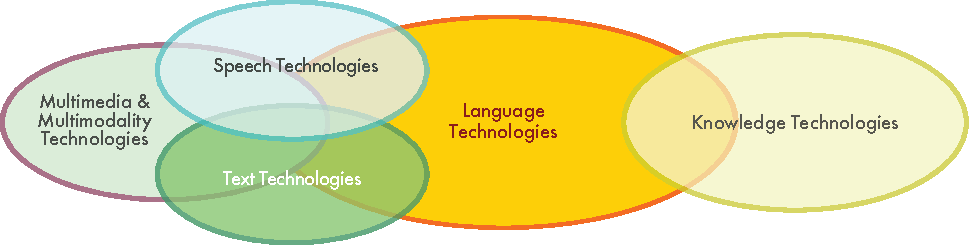
\includegraphics[width=\textwidth]{../_media/english/language_technologies}
  \caption{Language technologies}
  \label{fig:ltincontext_en}
  \colorrule{grey3}{\textwidth}{1.5pt}
\end{figure*}

Before discussing the above application areas, we will briefly describe the architecture of a typical LT system.

\subsection{Application Architectures}

\begin{figure*}[b]
  \colorrule{grey3}{\textwidth}{1.5pt}
  \center
  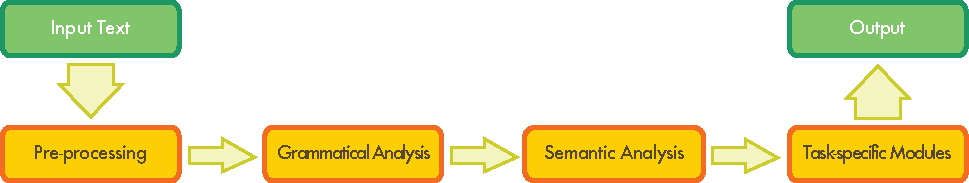
\includegraphics[width=\textwidth]{../_media/english/text_processing_app_architecture}
  \caption{A typical text processing architecture}
  \label{fig:textprocessingarch_en}
  \colorrule{grey3}{\textwidth}{1.5pt}
\end{figure*}

Typical software applications for language processing consist of several components that mirror different aspects of language and of the task they implement. Figure~\ref{fig:textprocessingarch_en} displays a highly simplified architecture that can be found in a text processing system. The first three modules deal with the structure and meaning of the text input:

\begin{itemize}
      \item Pre-processing: cleaning up the data, removing formatting, detecting the input language, etc. 
      \item Grammatical analysis: finding the verb and its objects, modifiers, etc.; detecting the sentence structure.
      \item Semantic analysis: disambiguation (Which meaning of \textit{apple} is the right one in a given context?), resolving anaphora and referring expressions like \textit{she, the car}, etc.; representing the meaning of the sentence in a machine readable way
\end{itemize}

 Task specific modules then perform many different operations such as automatic summarisation of an input text, database lookups and many others. Below, we will illustrate core application areas and highlight their core modules. Again, the architectures of the applications are highly simplified and idealised, to illustrate the complexity of language technology (LT) applications in a generally understandable way. 

After introducing the core application areas, we will give a short overview of the situation in LT research and education, concluding with an overview of past and ongoing research programs. At the end of this section, we will present an expert estimation on the situation regarding core LT tools and resources on a number of dimensions such as availability, maturity, or quality. 

%FIXME inserted:
The general situation of LT for the Galician language is summarised in figure~\ref{fig:lrlttable_en} (p.~\pageref{fig:lrlttable_en}) at the end of this chapter. This table lists all tools and resources that are boldfaced in the text.
%This table gives a good overview on the situation of LT for Galician.

%The most important tools and resources involved are in the text can be found in the table at the end of the chapter.
%The sections discussing the core application areas also contain an overview of the industries active in the respective field for Galician. 

\subsection{Core Application Areas}

In this section, we focus on the most important LT tools and resources, and give an overview of LT activities in Galician. %Tools and resources that are \textbf{boldface} in the text can also be found in figure \ref{fig:lrlttable_en} (p.~\pageref{fig:lrlttable_en}) at the end of this chapter.

\subsubsection{Language Checking}

\begin{figure*}[htb]
  \colorrule{grey3}{\textwidth}{1.5pt}
  \center
  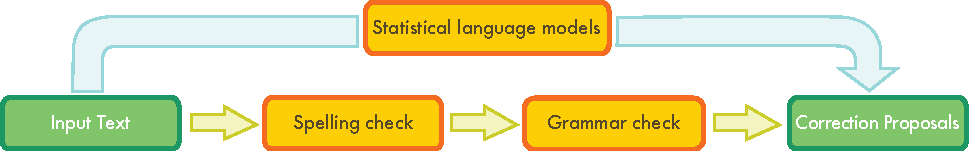
\includegraphics[width=\textwidth]{../_media/english/language_checking}
  \caption{Language checking (top: statistical; bottom: rule-based)}
  \label{fig:langcheckingaarch_en}
  \colorrule{grey3}{\textwidth}{1.5pt}
\end{figure*}

Anyone using a word processing tool such as Microsoft Word has come across a spell checking component that indicates spelling mistakes and proposes corrections. Forty years after the first spelling correction program by Ralph Gorin, language checkers nowadays do not simply compare the list of extracted words against a dictionary of correctly spelled words, but have become increasingly sophisticated. Using language-dependent algorithms for \textbf{grammatical analysis}, they handle mor\-pho\-lo\-gy (e.\,g., plural formation), some are now capable of recognising syntax related errors, such as a missing verb or a verb that does not agree with its subject in person and number, e.\,g., in ‘She *\textit{write} a letter.’ However, for other common error types, the above described methods are not sufficient. For example, take a look at the following first verse of a poem by Jerrold H.~Zar (1992): 

\boxtext{Language checkers have become increasingly sophisticated.}

\begin{verse}
\textit{Eye have a spelling chequer,} \\
\textit{It came with my Pea Sea.} \\
\textit{It plane lee marks four my revue} \\
\textit{Miss Steaks I can knot sea.}
\end{verse}

Most available spell checkers (including Microsoft Word) will find no errors in this poem because they mostly look at words in isolation. However, for detecting so called homophone errors (e.\,g., “Eye” instead of “I”), the language checker needs to consider the context in which a word occurs. For Galician, even spell checking requires analysing the context in many cases. A typical case is when the orthographic error transforms one word into another, which also exits. In the following example, the first sentence contains a frequent error (problems with orthographic accents). The second sentence is the corrected version of the first one.

\begin{itemize}
\item[] \textit{A casa do meu tío \textbf{e} a casa da miña avoa.}
\item[] \textit{[The house of my uncle and the house of my grandmother]}
\item[] \textit{A casa do meu tío \textbf{é} a casa da miña avoa.}
\item[] \textit{[The house of my uncle is the house of my grandmother]}
\end{itemize}

To automatically correct these errors, it is not enough to check each word in a dictionary, since all words in the first sentence are correct in isolation. This either requires the formulation of language-specific \textbf{grammars}, i.\,e., a high degree of expertise and manual labour, or the use of a so called statistical language model. Such models calculate the probability of a particular word occurring in a specific environment (i.\,e., the preceding and following words). For example, “é a” is a much more probable word sequence than “e a”. A statistical language model can be derived automatically using a large amount of (correct) language data (i.\,e., a \textbf{text corpus}).

Up to now, these approaches have mostly been developed and evaluated on English language data. However, they do not necessarily transfer well to other languages, e.\,g., highly inflectional ones or languages with a flexible word order like Galician. For these more complex languages, an advanced high-precision language checker may require the development of more sophisticated methods, involving a deeper linguistic analysis.

The use of Language Checking is not limited to word processing tools. It is also applied in authoring support systems. Accompanying the rising number of technical products, the amount of technical documentation has rapidly increased over the last decades. Fearing customer complaints about wrong usage and damage claims resulting from bad or badly understood instructions, companies have begun to focus increasingly on the quality of technical documentation, and at the same time targeting the international market. Advances in natural language processing lead to the development of authoring support software, which assists the writer of technical documentation to use vocabulary and sentence structures consistent with certain rules and (corporate) terminology restrictions. 

\boxtext{Language checking is not limited to word processors but also applies to authoring systems.}

Only few companies and Language Service Providers offer products in this area for Galician.  \textit{Imaxin software} \cite{GAL-Nota21} is one example with some online free-to-use services for translation and grammar checking. \textit{OrtoGal} software from Computational Linguistics Group (SLI) \cite{GAL-Nota22} of the University of Vigo offers spell and grammar checking. There is also plug-in software for OpenOffice like \textit{Golfiño} \cite{GAL-Nota23} developed by \textit{Imaxin Software} and supported by the Galician Regional Government.

Besides spell checkers and authoring support, Language Checking is also important in the field of computer-assisted language learning and is applied to automatically correct queries sent to web search engines, e.\,g., Google’s ‘Did you mean…’ suggestions. 

\subsubsection{Web Search}

\begin{figure*}[htb]
  \colorrule{grey3}{\textwidth}{1.5pt}
  \center
  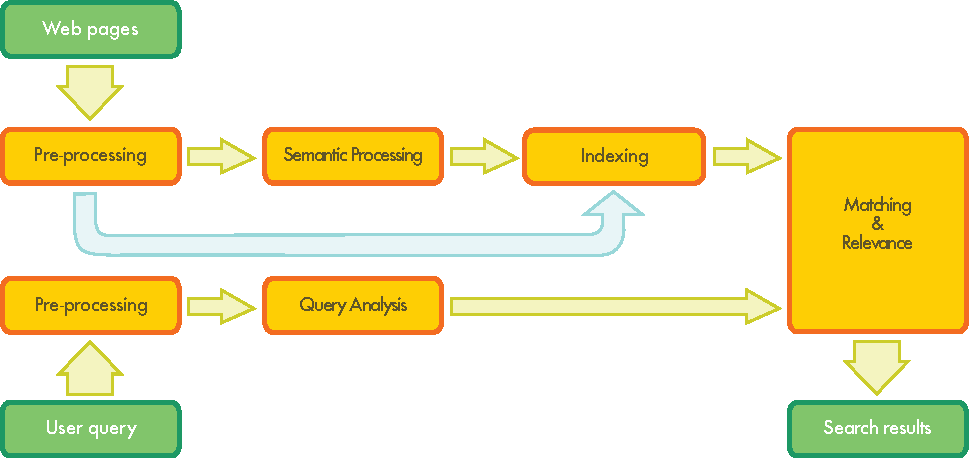
\includegraphics[width=\textwidth]{../_media/english/web_search_architecture}
  \caption{Web search}
  \label{fig:websearcharch_en}
  \colorrule{grey3}{\textwidth}{1.5pt}
 \end{figure*}

   Search on the web, in intranets, or in digital libraries is probably the most widely used and yet underdeveloped language technology today. The search engine Google, which started in 1998, is nowadays used for about 80\% of all search queries world wide. Neither the search interface nor the presentation of the retrieved results has significantly changed since the first version. In the current version, Google offers a spelling correction for misspelled words also for Galician and, in 2009, they incorporated basic semantic search capabilities into their algorithmic mix, which can improve search accuracy by analysing the meaning of the query terms in context. The success story of Google shows that with a lot of data at hand and efficient techniques for indexing these data, a mainly statistically based approach can lead to satisfactory results. 

However, for a more sophisticated request for information, integrating deeper linguistic knowledge is essential. In the research labs, experiments using \textbf{lexical resources} such as machine readable thesauri and ontological language resources like WordNet have shown improvements by allowing the possibility of finding a page on the basis of synonyms of the search terms, or even more loosely related terms. Again, these developments require of language specific resources. A Galician WordNet has been developed by the research centre “Centro Ramón Piñeiro para la Investigación en Humanidades” \cite{GAL-Nota24}. The Galician WordNet is called GALWORDNET.

The next generation of search engines will have to include much more sophisticated language technology. If a search query consists of a question or another type of sentence rather than a list of keywords, retrieving relevant answers to this query requires a syntactic and \textbf{semantic analysis} of the sentence, as well as the availability of an index that allows for a fast retrieval of the relevant documents. For example, imagine a user inputs the query ‘Give me a list of all companies that were taken over by other companies in the last five years’. For a satisfactory answer, syntactic parsing needs to be applied to analyse the grammatical structure of the sentence and determine that the user is looking for companies that have been taken over and not companies that took over others. Also, the expression \textit{last five years} needs to be processed in order to find out which years it refers to. 

Finally, the processed query needs to be matched against a huge amount of unstructured data in order to find the piece or pieces of information the user is looking for. This is commonly referred to as information retrieval and involves the search for and ranking of relevant documents. In addition, generating a list of companies, we also need to extract the information that a particular string of words in a document refers to a company name. This kind of information is made available by so called named entity recognisers.

\boxtext{The next generation of search engines\\ will have to include much more sophisticated language technology.}

Even more demanding is the attempt to match a query to documents written in a different language. For \textbf{cross-lingual information retrieval}, we have to automatically translate the query to all possible source languages and transfer the retrieved information back to the target language. The increasing percentage of data available in non-textual formats drives the demand for services enabling \textbf{multimedia information retrieval}, i.\,e., information search on images, audio, and video data. For audio and video files, this involves a \textbf{speech recognition} module to convert speech content into text or a phonetic representation, to which user queries can be matched.

To the best of our knowledge there is no linguistic technology at companies aimed at multilingual search and information retrieval, both from the Internet and from internal information systems on Galician.  


\subsubsection{Speech Interaction}

\begin{figure*}[htb]
  \colorrule{grey3}{\textwidth}{1.5pt}
  \center
  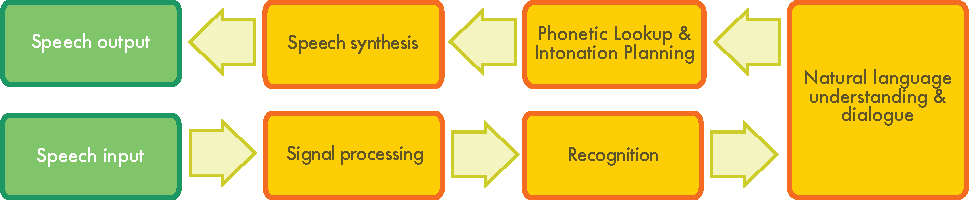
\includegraphics[width=\textwidth]{../_media/english/simple_speech-based_dialogue_architecture}
  \caption{Speech-based dialogue system}
  \label{fig:dialoguearch_en}
  \colorrule{grey3}{\textwidth}{1.5pt}
\end{figure*}

Speech interaction technology is the basis for the creation of interfaces that allow a user to interact with machines using spoken language rather than, e.\,g., a graphical display, a keyboard and a mouse. Today, such voice user interfaces (VUIs) are usually employed for partially or fully automating service offerings provided by companies to their customers, employees or partners via the telephone. Business domains that rely heavily on VUIs are banking, logistics, public transportation and telecommunications. Other usages of speech interaction technology are interfaces to particular devices, e.\,g., in car navigation systems, and the employment of spoken language as an alternative to the input/output modalities of graphical user interfaces, e.\,g., in smart phones.

At its core, speech interaction comprises the following four different technologies:

\begin{itemize}
\item Automatic \textbf{speech recognition} (ASR) is responsible for determining which words were actually spoken given a sequence of sounds uttered by a user.
\item Syntactic analysis and semantic interpretation deal with analysing the syntactic structure of a user’s utterance and interpretting the latter according to the given system’s purpose.
\item Dialogue Management is required for determining, on the part of the system the user interacts with, which action shall be taken given the user’s input and the system’s functionality.
\item \textbf{Speech Synthesis} (Text-to-Speech, TTS) technology is employed for transforming the wording of that utterance into sounds that will be output to the user. 
\end{itemize}

One of the major challenges is to have an ASR system recognise the words uttered by a user as precisely as possible. This requires either a restriction of the range of possible user utterances to a limited set of keywords, or the manual creation of language models that cover a large range of natural language user utterances. Using machine learning techniques, language models can also be generated automatically from \textbf{speech corpora}, i.\,e., large collections of speech audio files and text transcriptions.

Whereas the former results in a rather rigid and inflexible usage of a VUI and possibly causes a poor user acceptance, the creation, tuning and maintenance of language models may increase the costs significantly. However, VUIs that employ language models and initially allow a user to flexibly express their intent – evoked, e.\,g., by a \textit{How may I help you} greeting – show both a higher automation rate and a higher user acceptance and may therefore be considered as advantageous over a less flexible \textit{directed dialogue} approach.

\boxtext{Speech interaction is the basis for interfaces that allow a user to interact with spoken language.}

For the output part of a VUI, companies tend to use utterances pre-recorded by professional – ideally corporate – speakers a lot. For static utterances, in which the wording does not depend on the particular contexts of use or the personal data of the given user, this will result in a rich user experience. However, the more dynamic content an utterance needs to consider, the more the user experience may suffer from a poor prosody resulting from concatenating single audio files. In contrast, today’s TTS systems prove superior, though optimisable, regarding the prosodic naturalness of dynamic utterances.  

Regarding the market for speech interaction technology, the last decade has been characterised by a strong standardisation of the interfaces between the different technology components, as well as by standards for creating particular software artefacts for a given application. There also has been strong market consolidation within the last ten years, particularly in the field of ASR and TTS. Here, the national markets in the G20 countries – i.\,e., economically strong countries with a considerable population -- are dominated by less than 5 players worldwide, with \textit{Nuance and Loquendo} being the most prominent ones in Europe, also for Galician (Loquendo), although some smaller local companies are starting to compete, such as Verbio \cite{GAL-Nota25} , which is a spin-off of Universitat Politècnica de Catalunya and has its own speech technology, or the Galician \textit{2Mares} \cite{GAL-Nota26}. 

Regarding dialogue management technology and know-how, markets are strongly dominated by national players, which are usually SMEs.
Most of the companies on the Spanish TTS market (some offer Galician) are essentially application developers. Key players in the Spanish market are: Indsys \cite{GAL-Nota27} (Intelligent Dialogue Systems), Fonetic \cite{GAL-Nota28}, Ydilo \cite{GAL-Nota29}, NaturalVoz \cite{GAL-Nota30}, and 2Mares.

Looking beyond today’s state of technology, there will be significant changes due to the spread of smart phones as a new platform for managing customer relationships – in addition to the telephone, Internet, and e-mail channels. This tendency will also affect the employment of technology for speech interaction. On one hand, demand for telephony-based VUIs will decrease, in the long run. On the other hand, the usage of spoken language as a user-friendly input modality for smart phones will gain significant importance. This tendency is supported by the observable improvement of speaker independent speech recognition accuracy for speech dictation services that are already offered as centralised services to smart phone users. Given this outsourcing of the recognition task to the infrastructure of applications, the application-specific employment of linguistic core technologies will supposedly gain importance compared to the present situation. 

\subsubsection{Machine Translation}

The idea of using digital computers for translation of natural languages came up in 1946 by A.~D.~Booth and was followed by substantial funding for research in this area in the 1950s and beginning again in the 1980s. Nevertheless, \textbf{Machine Translation} (MT) still fails to fulfil the high expectations it gave rise to in its early years. 

\boxtext{At its basic level, Machine Translation simply substitutes words in one natural language with words in another language.}

\begin{figure*}[htb]
  \colorrule{grey3}{\textwidth}{1.5pt}
  \center
  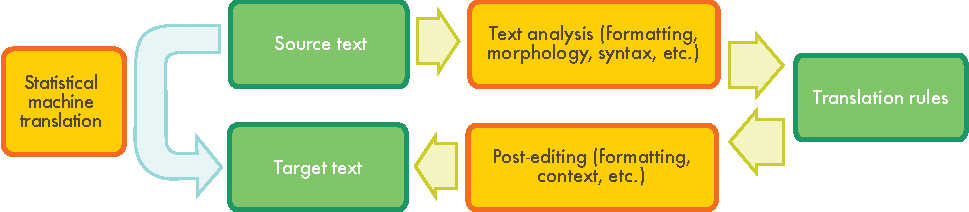
\includegraphics[width=\textwidth]{../_media/english/machine_translation}
  \caption{Machine translation (left: statistical; right: rule-based)}
  \label{fig:mtarch_en}
  \colorrule{grey3}{\textwidth}{1.5pt}
\end{figure*}

At its basic level, MT simply substitutes words in one natural language by words in another. This can be useful in subject domains with a very restricted, formulaic language, e.\,g., weather reports. However, for a good translation of less standardised texts, larger text units (phrases, sentences, or even whole passages) need to be matched to their closest counterparts in the target language. The major difficulty here lies in the fact that human language is ambiguous, which yields challenges on multiple levels, e.\,g., word sense disambiguation at the lexical level (‘Jaguar’ can mean a car or an animal) or on other levels as in:

\begin{itemize}
\item[] \textit{O policía observou ao home co telescopio.}
\item[] \textit{[The policeman observed the man with the telescope.]}
\item[] \textit{O policía observou ao home co revólver.}
\item[] \textit{[The policeman observed the man with the revolver.]}
\end{itemize}

One way of approaching the task is based on linguistic rules. For translations between closely related languages, a direct translation may be feasible in cases like the example above. But often rule-based (or knowledge-driven) systems analyse the input text and create an intermediary, symbolic representation, from which the text in the target language is generated. The success of these methods is highly dependent on the availability of extensive lexicons with morphological, syntactic, and semantic information, and large sets of grammar rules carefully designed by a skilled linguist.

Beginning in the late 1980s, as computational power increased and became less expensive, more interest was shown in statistical models for MT. The parameters of these statistical models are derived from the analysis of bilingual text \textbf{parallel corpora}, such as the Europarl parallel corpus, which contains the proceedings of the European Parliament in 21 European languages. Given enough data, statistical MT works well enough to derive an approximate meaning of a foreign language text. However, unlike knowledge-driven systems, statistical (or data-driven) MT often generates ungrammatical output. On the other hand, besides the advantage that less human effort is required for grammar writing, data-driven MT can also cover particularities of the language that go missing in knowledge-driven systems, for example idiomatic expressions. 

As the strengths and weaknesses of knowledge- and data-driven MT are complementary, researchers nowadays unanimously target hybrid approaches combining methodologies of both. This can be done in several ways. One is to use both knowledge- and data-driven systems and have a selection module decide on the best output for each sentence. However, for longer sentences, no result will be perfect. A better solution is to combine the best parts of each sentence from multiple outputs, which can be fairly complex, as corresponding parts of multiple alternatives are not always obvious and need to be aligned. 

Leading international MT developer Lucy Software has an important subsidiary in Spain, Lucy Iberica \cite{GAL-Nota31}, former Translendium. Lucy Iberica is responsible for the development of language pairs that include Spanish and all language pairs involving any other Iberian language (Catalan, Portuguese, Galician and Basque). Lucy system is grammar rule-based. The Regional Government (“Xunta de Galicia”) \cite{GAL-Nota32} offers a translation service on the Internet that uses the technology of the Lucy Iberica. While there is significant research in data-driven and hybrid systems in national and international contexts, this technology has been less successful in business than in research so far.

Apertium is a free open-source machine translation platform that provides a language-independent machine translation engine initially designed by the Transducens group at the Universitat d'Alacant and subsequently developed in the framework of the nationally funded Opentrad project. Among current MT systems using Apertium technology, we find interNOSTRUM (Spanish-Catalan), Traductor Universia (Spanish-Portuguese) and Matxin (Basque-Spanish), the former developed by Transducens and the latter by the IXA group \cite{GAL-Nota33} at Euskal Herriko Unibertsitatea, Imaxin Software (Galician-Spanish). It is possible to use Apertium to build machine translation systems for a variety of language pairs (there are over 20 to date); to that end, Apertium uses simple XML-based standard formats to encode the linguistic data needed (either by hand or by converting existing data), which are compiled using the provided tools into the high-speed formats used by the engine.

Provided good adaptation in terms of user-specific terminology and workflow integration, there is a wide consensus that the use of MT can increase productivity significantly. The quality of MT systems is still considered to have huge improvement potential. Challenges include the adaptability of the language resources to a given subject domain or user area and the integration into existing workflows with term bases and translation memories. In addition, many language pairs are still missing. 
%
%\begin{figure*}[tb]
%  \centering
%  \setlength{\tabcolsep}{0.17em}
%  \small
%  \begin{tabular}{>{\columncolor{corange1}}cccccccccccccccccccccccc}
%    & \multicolumn{22}{>{\columncolor{corange1}}c}{Target language -- \textcolor{grey1}{Target language}}\\\addlinespace[{-.009cm}]
%    \rowcolor{corange1}  & EN & BG & DE & CS & DA & EL & ES & ET & FI & FR & HU & IT & LT & LV & MT & NL & PL & PT & RO & SK & SL & SV\\
%    EN & -- & \textcolor{blue}{40.5} & \textcolor{blue}{46.8} & \textcolor{green2}{52.6} & \textcolor{green2}{50.0} & \textcolor{blue}{41.0} & \textcolor{green2}{55.2} & \textcolor{purple}{34.8} & \textcolor{purple}{38.6} & \textcolor{green2}{50.1} & \textcolor{purple}{37.2} & \textcolor{green2}{50.4} & \textcolor{purple}{39.6} & \textcolor{blue}{43.4} & \textcolor{purple}{39.8} & \textcolor{green2}{52.3} & \textcolor{blue}{49.2} & \textcolor{green2}{55.0} & \textcolor{blue}{49.0} & \textcolor{blue}{44.7} & \textcolor{green2}{50.7} & \textcolor{green2}{52.0}\\
%    BG & \textcolor{green}{61.3} & -- & \textcolor{purple}{38.7} & \textcolor{purple}{39.4} & \textcolor{purple}{39.6} & \textcolor{purple}{34.5} & \textcolor{blue}{46.9} & \textcolor{red3}{25.5} & \textcolor{red3}{26.7} & \textcolor{blue}{42.4} & \textcolor{red3}{22.0} & \textcolor{blue}{43.5} & \textcolor{red3}{29.3} & \textcolor{red3}{29.1} & \textcolor{red3}{25.9} & \textcolor{blue}{44.9} & \textcolor{purple}{35.1} & \textcolor{blue}{45.9} & \textcolor{purple}{36.8} & \textcolor{purple}{34.1} & \textcolor{purple}{34.1} & \textcolor{purple}{39.9}\\
%    DE & \textcolor{green2}{53.6} & \textcolor{red3}{26.3} & -- & \textcolor{purple}{35.4} & \textcolor{blue}{43.1} & \textcolor{purple}{32.8} & \textcolor{blue}{47.1} & \textcolor{red3}{26.7} & \textcolor{red3}{29.5} & \textcolor{purple}{39.4} & \textcolor{red3}{27.6} & \textcolor{blue}{42.7} & \textcolor{red3}{27.6} & \textcolor{purple}{30.3} & \textcolor{red2}{19.8} & \textcolor{green2}{50.2} & \textcolor{purple}{30.2} & \textcolor{blue}{44.1} & \textcolor{purple}{30.7} & \textcolor{red3}{29.4} & \textcolor{purple}{31.4} & \textcolor{blue}{41.2}\\
%    CS & \textcolor{green2}{58.4} & \textcolor{purple}{32.0} & \textcolor{blue}{42.6} & -- & \textcolor{blue}{43.6} & \textcolor{purple}{34.6} & \textcolor{blue}{48.9} & \textcolor{purple}{30.7} & \textcolor{purple}{30.5} & \textcolor{blue}{41.6} & \textcolor{red3}{27.4} & \textcolor{blue}{44.3} & \textcolor{purple}{34.5} & \textcolor{purple}{35.8} & \textcolor{red3}{26.3} & \textcolor{blue}{46.5} & \textcolor{purple}{39.2} & \textcolor{blue}{45.7} & \textcolor{purple}{36.5} & \textcolor{blue}{43.6} & \textcolor{blue}{41.3} & \textcolor{blue}{42.9}\\
%    DA & \textcolor{green2}{57.6} & \textcolor{red3}{28.7} & \textcolor{blue}{44.1} & \textcolor{purple}{35.7} & -- & \textcolor{purple}{34.3} & \textcolor{blue}{47.5} & \textcolor{red3}{27.8} & \textcolor{purple}{31.6} & \textcolor{blue}{41.3} & \textcolor{red3}{24.2} & \textcolor{blue}{43.8} & \textcolor{red3}{29.7} & \textcolor{purple}{32.9} & \textcolor{red3}{21.1} & \textcolor{blue}{48.5} & \textcolor{purple}{34.3} & \textcolor{blue}{45.4} & \textcolor{purple}{33.9} & \textcolor{purple}{33.0} & \textcolor{purple}{36.2} & \textcolor{blue}{47.2}\\
%    EL & \textcolor{green2}{59.5} & \textcolor{purple}{32.4} & \textcolor{blue}{43.1} & \textcolor{purple}{37.7} & \textcolor{blue}{44.5} & -- & \textcolor{green2}{54.0} & \textcolor{red3}{26.5} & \textcolor{red3}{29.0} & \textcolor{blue}{48.3} & \textcolor{red3}{23.7} & \textcolor{blue}{49.6} & \textcolor{red3}{29.0} & \textcolor{purple}{32.6} & \textcolor{red3}{23.8} & \textcolor{blue}{48.9} & \textcolor{purple}{34.2} & \textcolor{green2}{52.5} & \textcolor{purple}{37.2} & \textcolor{purple}{33.1} & \textcolor{purple}{36.3} & \textcolor{blue}{43.3}\\
%    ES & \textcolor{green}{60.0} & \textcolor{purple}{31.1} & \textcolor{blue}{42.7} & \textcolor{purple}{37.5} & \textcolor{blue}{44.4} & \textcolor{purple}{39.4} & -- & \textcolor{red3}{25.4} & \textcolor{red3}{28.5} & \textcolor{green2}{51.3} & \textcolor{red3}{24.0} & \textcolor{green2}{51.7} & \textcolor{red3}{26.8} & \textcolor{purple}{30.5} & \textcolor{red3}{24.6} & \textcolor{blue}{48.8} & \textcolor{purple}{33.9} & \textcolor{green2}{57.3} & \textcolor{purple}{38.1} & \textcolor{purple}{31.7} & \textcolor{purple}{33.9} & \textcolor{blue}{43.7}\\
%    ET & \textcolor{green2}{52.0} & \textcolor{red3}{24.6} & \textcolor{purple}{37.3} & \textcolor{purple}{35.2} & \textcolor{purple}{37.8} & \textcolor{red3}{28.2} & \textcolor{blue}{40.4} & -- & \textcolor{purple}{37.7} & \textcolor{purple}{33.4} & \textcolor{purple}{30.9} & \textcolor{purple}{37.0} & \textcolor{purple}{35.0} & \textcolor{purple}{36.9} & \textcolor{red3}{20.5} & \textcolor{blue}{41.3} & \textcolor{purple}{32.0} & \textcolor{purple}{37.8} & \textcolor{red3}{28.0} & \textcolor{purple}{30.6} & \textcolor{purple}{32.9} & \textcolor{purple}{37.3}\\
%    FI & \textcolor{blue}{49.3} & \textcolor{red3}{23.2} & \textcolor{purple}{36.0} & \textcolor{purple}{32.0} & \textcolor{purple}{37.9} & \textcolor{red3}{27.2} & \textcolor{purple}{39.7} & \textcolor{purple}{34.9} & -- & \textcolor{red3}{29.5} & \textcolor{red3}{27.2} & \textcolor{purple}{36.6} & \textcolor{purple}{30.5} & \textcolor{purple}{32.5} & \textcolor{red2}{19.4} & \textcolor{blue}{40.6} & \textcolor{red3}{28.8} & \textcolor{purple}{37.5} & \textcolor{red3}{26.5} & \textcolor{red3}{27.3} & \textcolor{red3}{28.2} & \textcolor{purple}{37.6}\\
%    FR & \textcolor{green}{64.0} & \textcolor{purple}{34.5} & \textcolor{blue}{45.1} & \textcolor{purple}{39.5} & \textcolor{blue}{47.4} & \textcolor{blue}{42.8} & \textcolor{green}{60.9} & \textcolor{red3}{26.7} & \textcolor{purple}{30.0} & -- & \textcolor{red3}{25.5} & \textcolor{green2}{56.1} & \textcolor{red3}{28.3} & \textcolor{purple}{31.9} & \textcolor{red3}{25.3} & \textcolor{green2}{51.6} & \textcolor{purple}{35.7} & \textcolor{green}{61.0} & \textcolor{blue}{43.8} & \textcolor{purple}{33.1} & \textcolor{purple}{35.6} & \textcolor{blue}{45.8}\\
%    HU & \textcolor{blue}{48.0} & \textcolor{red3}{24.7} & \textcolor{purple}{34.3} & \textcolor{purple}{30.0} & \textcolor{purple}{33.0} & \textcolor{red3}{25.5} & \textcolor{purple}{34.1} & \textcolor{red3}{29.6} & \textcolor{red3}{29.4} & \textcolor{purple}{30.7} & -- & \textcolor{purple}{33.5} & \textcolor{red3}{29.6} & \textcolor{purple}{31.9} & \textcolor{red2}{18.1} & \textcolor{purple}{36.1} & \textcolor{red3}{29.8} & \textcolor{purple}{34.2} & \textcolor{red3}{25.7} & \textcolor{red3}{25.6} & \textcolor{red3}{28.2} & \textcolor{purple}{30.5}\\
%    IT & \textcolor{green}{61.0} & \textcolor{purple}{32.1} & \textcolor{blue}{44.3} & \textcolor{purple}{38.9} & \textcolor{blue}{45.8} & \textcolor{blue}{40.6} & \textcolor{red3}{26.9} & \textcolor{red3}{25.0} & \textcolor{red3}{29.7} & \textcolor{green2}{52.7} & \textcolor{red3}{24.2} & -- & \textcolor{red3}{29.4} & \textcolor{purple}{32.6} & \textcolor{red3}{24.6} & \textcolor{green2}{50.5} & \textcolor{purple}{35.2} & \textcolor{green2}{56.5} & \textcolor{purple}{39.3} & \textcolor{purple}{32.5} & \textcolor{purple}{34.7} & \textcolor{blue}{44.3}\\
%    LT & \textcolor{green2}{51.8} & \textcolor{red3}{27.6} & \textcolor{purple}{33.9} & \textcolor{purple}{37.0} & \textcolor{purple}{36.8} & \textcolor{red3}{26.5} & \textcolor{red3}{21.1} & \textcolor{purple}{34.2} & \textcolor{purple}{32.0} & \textcolor{purple}{34.4} & \textcolor{red3}{28.5} & \textcolor{purple}{36.8} & -- & \textcolor{blue}{40.1} & \textcolor{red3}{22.2} & \textcolor{purple}{38.1} & \textcolor{purple}{31.6} & \textcolor{purple}{31.6} & \textcolor{red3}{29.3} & \textcolor{purple}{31.8} & \textcolor{purple}{35.3} & \textcolor{purple}{35.3}\\
%    LV & \textcolor{green2}{54.0} & \textcolor{red3}{29.1} & \textcolor{purple}{35.0} & \textcolor{purple}{37.8} & \textcolor{purple}{38.5} & \textcolor{red3}{29.7} & \textcolor{red2}{8.0} & \textcolor{purple}{34.2} & \textcolor{purple}{32.4} & \textcolor{purple}{35.6} & \textcolor{red3}{29.3} & \textcolor{purple}{38.9} & \textcolor{purple}{38.4} & -- & \textcolor{red3}{23.3} & \textcolor{blue}{41.5} & \textcolor{purple}{34.4} & \textcolor{purple}{39.6} & \textcolor{purple}{31.0} & \textcolor{purple}{33.3} & \textcolor{purple}{37.1} & \textcolor{purple}{38.0}\\
%    MT & \textcolor{green}{72.1} & \textcolor{purple}{32.2} & \textcolor{purple}{37.2} & \textcolor{purple}{37.9} & \textcolor{purple}{38.9} & \textcolor{purple}{33.7} & \textcolor{blue}{48.7} & \textcolor{red3}{26.9} & \textcolor{red3}{25.8} & \textcolor{blue}{42.4} & \textcolor{red3}{22.4} & \textcolor{blue}{43.7} & \textcolor{purple}{30.2} & \textcolor{purple}{33.2} & -- & \textcolor{blue}{44.0} & \textcolor{purple}{37.1} & \textcolor{blue}{45.9} & \textcolor{purple}{38.9} & \textcolor{purple}{35.8} & \textcolor{blue}{40.0} & \textcolor{blue}{41.6}\\
%    NL & \textcolor{green2}{56.9} & \textcolor{red3}{29.3} & \textcolor{blue}{46.9} & \textcolor{purple}{37.0} & \textcolor{blue}{45.4} & \textcolor{purple}{35.3} & \textcolor{blue}{49.7} & \textcolor{red3}{27.5} & \textcolor{red3}{29.8} & \textcolor{blue}{43.4} & \textcolor{red3}{25.3} & \textcolor{blue}{44.5} & \textcolor{red3}{28.6} & \textcolor{purple}{31.7} & \textcolor{red3}{22.0} & -- & \textcolor{purple}{32.0} & \textcolor{blue}{47.7} & \textcolor{purple}{33.0} & \textcolor{purple}{30.1} & \textcolor{purple}{34.6} & \textcolor{blue}{43.6}\\
%    PL & \textcolor{green}{60.8} & \textcolor{purple}{31.5} & \textcolor{blue}{40.2} & \textcolor{blue}{44.2} & \textcolor{blue}{42.1} & \textcolor{purple}{34.2} & \textcolor{blue}{46.2} & \textcolor{red3}{29.2} & \textcolor{red3}{29.0} & \textcolor{blue}{40.0} & \textcolor{red3}{24.5} & \textcolor{blue}{43.2} & \textcolor{purple}{33.2} & \textcolor{purple}{35.6} & \textcolor{red3}{27.9} & \textcolor{blue}{44.8} & -- & \textcolor{blue}{44.1} & \textcolor{purple}{38.2} & \textcolor{purple}{38.2} & \textcolor{purple}{39.8} & \textcolor{blue}{42.1}\\
%    PT & \textcolor{green}{60.7} & \textcolor{purple}{31.4} & \textcolor{blue}{42.9} & \textcolor{purple}{38.4} & \textcolor{blue}{42.8} & \textcolor{blue}{40.2} & \textcolor{green}{60.7} & \textcolor{red3}{26.4} & \textcolor{red3}{29.2} & \textcolor{green2}{53.2} & \textcolor{red3}{23.8} & \textcolor{green2}{52.8} & \textcolor{red3}{28.0} & \textcolor{purple}{31.5} & \textcolor{red3}{24.8} & \textcolor{blue}{49.3} & \textcolor{purple}{34.5} & -- & \textcolor{purple}{39.4} & \textcolor{purple}{32.1} & \textcolor{purple}{34.4} & \textcolor{blue}{43.9}\\
%    RO & \textcolor{green}{60.8} & \textcolor{purple}{33.1} & \textcolor{purple}{38.5} & \textcolor{purple}{37.8} & \textcolor{blue}{40.3} & \textcolor{purple}{35.6} & \textcolor{green2}{50.4} & \textcolor{red3}{24.6} & \textcolor{red3}{26.2} & \textcolor{blue}{46.5} & \textcolor{red3}{25.0} & \textcolor{blue}{44.8} & \textcolor{red3}{28.4} & \textcolor{red3}{29.9} & \textcolor{red3}{28.7} & \textcolor{blue}{43.0} & \textcolor{purple}{35.8} & \textcolor{blue}{48.5} & -- & \textcolor{purple}{31.5} & \textcolor{purple}{35.1} & \textcolor{purple}{39.4}\\
%    SK & \textcolor{green}{60.8} & \textcolor{purple}{32.6} & \textcolor{purple}{39.4} & \textcolor{blue}{48.1} & \textcolor{blue}{41.0} & \textcolor{purple}{33.3} & \textcolor{blue}{46.2} & \textcolor{red3}{29.8} & \textcolor{red3}{28.4} & \textcolor{purple}{39.4} & \textcolor{red3}{27.4} & \textcolor{blue}{41.8} & \textcolor{purple}{33.8} & \textcolor{purple}{36.7} & \textcolor{red3}{28.5} & \textcolor{blue}{44.4} & \textcolor{purple}{39.0} & \textcolor{blue}{43.3} & \textcolor{purple}{35.3} & -- & \textcolor{blue}{42.6} & \textcolor{blue}{41.8}\\
%    SL & \textcolor{green}{61.0} & \textcolor{purple}{33.1} & \textcolor{purple}{37.9} & \textcolor{blue}{43.5} & \textcolor{blue}{42.6} & \textcolor{purple}{34.0} & \textcolor{blue}{47.0} & \textcolor{purple}{31.1} & \textcolor{red3}{28.8} & \textcolor{purple}{38.2} & \textcolor{red3}{25.7} & \textcolor{blue}{42.3} & \textcolor{purple}{34.6} & \textcolor{purple}{37.3} & \textcolor{purple}{30.0} & \textcolor{blue}{45.9} & \textcolor{purple}{38.2} & \textcolor{blue}{44.1} & \textcolor{purple}{35.8} & \textcolor{purple}{38.9} & -- & \textcolor{blue}{42.7}\\
%    SV & \textcolor{green2}{58.5} & \textcolor{red3}{26.9} & \textcolor{blue}{41.0} & \textcolor{purple}{35.6} & \textcolor{blue}{46.6} & \textcolor{purple}{33.3} & \textcolor{blue}{46.6} & \textcolor{red3}{27.4} & \textcolor{purple}{30.9} & \textcolor{purple}{38.9} & \textcolor{red3}{22.7} & \textcolor{blue}{42.0} & \textcolor{red3}{28.2} & \textcolor{purple}{31.0} & \textcolor{red3}{23.7} & \textcolor{blue}{45.6} & \textcolor{purple}{32.2} & \textcolor{blue}{44.2} & \textcolor{purple}{32.7} & \textcolor{purple}{31.3} & \textcolor{purple}{33.5} & --\\
%    \end{tabular}
%  \caption{Machine translation between 22 EU-languages \cite{euro1}}
%  \label{fig:euromatrix_en}
%\end{figure*}

Evaluation campaigns help to compare the quality of MT systems, their approaches and the status of the systems for different language pairs. Figure~\ref{fig:euromatrix_gal} (p.~\pageref{fig:euromatrix_gal}), which was prepared during the Euromatrix+ project, shows the pair-wise performances obtained for 22 of the 23 EU languages (Irish was not compared). The results are ranked according to a BLEU score, which indicates higher scores for better translations \cite{bleu1}. A human translator would normally achieve around 80 points. The best results (in green and blue) were achieved by languages that benefit from a considerable research effort in coordinated programmes and the existence of many parallel corpora (e.\,g., English, French, Dutch, Spanish and German). The languages with poorer results are shown in red. These either lack such development efforts or are structurally very different from other languages (e.\,g., Hungarian, Maltese, Finnish).

\subsection{Other Application Areas}

Building Language Technology applications involves a range of subtasks that do not always surface at the level of interaction with the user, but provide significant service functionalities ‘under the hood’ of the system. Therefore, they constitute important research issues that have become individual sub-disciplines of Computational Linguistics in academia. 

Question answering has become an active area of research, for which annotated corpora have been built and scientific competitions have been started.

The idea is to move from keyword based search (to which the engine responds with a whole collection of potentially relevant documents) to the scenario of the user asking a concrete question and the system providing a single answer:

\begin{itemize}
\item[] \textit{Question: At what age did Neil Armstrong step on the moon?}
\item[] \textit{Answer: 38.}
\end{itemize}

While this is obviously related to the aforementioned core area web search, question answering nowadays is primarily an umbrella term for research questions such as what types of questions should be distinguished and how should they be handled, how can a set of documents that potentially contain the answer be analysed and compared (do they give conflicting answers?), and how can specific information -- the answer -- be reliably extracted from a document, without unduly ignoring the context. 

This is in turn related to the information extraction (IE) task, an area that was extremely popular and influential at the time of the ‘statistical turn’ in Computational Linguistics, in the early 1990s. IE aims at identifying specific pieces of information in specific classes of documents; this could e.\,g., be the detection of the key players in company takeovers as reported in newspaper stories. Another scenario that has been worked on is reports on terrorist incidents, where the problem is to map the text to a template specifying the perpetrator, the target, time and location of the incident, and the results of the incident. Domain-specific template-filling is the central characteristic of IE, which for this reason is another example of a ‘behind the scenes’ technology that constitutes a well demarcated research area but for practical purposes then needs to be embedded into a suitable application environment. 

\boxtext{Language technology applications often provide significant service functionalities behind the scenes of larger software systems.}

Two borderline areas, which sometimes play the role of standalone application and sometimes that of supportive, ‘under the hood’ component are text summarisation and \textbf{text generation}. Summarisation, obviously, refers to the task of making a long text short, and is offered for instance as a functionality within MS Word. It works largely on a statistical basis, by first identifying ‘important’ words in a text (that is, for example, words that are highly frequent in this text but markedly less frequent in general language use) and then determining those sentences that contain many important words. These sentences are then marked in the document, or extracted from it, and are taken to constitute the summary. In this scenario, which is by far the most popular one, summarisation equals sentence extraction: the text is reduced to a subset of its sentences. All commercial summarisers make use of this idea. An alternative approach, to which some research is devoted, is to actually synthesize \textit{new} sentences, i.\,e., to build a summary of sentences that need not show up in that form in the source text. This requires a certain amount of deeper understanding of the text and therefore is much less robust. All in all, a text generator is in most cases not a standalone application but embedded into a larger software environment, such as into the clinical information system where patient data is collected, stored and processed, and report generation is just one of many functionalities.

\boxtext{For Galician and for most languages, research in most text technologies is much less developed than for English.}

For Galician, the situation in these research areas is much less developed than it is for English, where, since the 1990s, question answering, information extraction, and summarisation have been the subject of numerous open competitions, primarily those organised by DARPA/NIST in the United States. These have significantly improved the state of the art, but the focus has always been on English; some competitions have added multilingual tracks, but Galician was never a targeted language. Accordingly, there are hardly any annotated corpora or other resources for these tasks. Summarisation systems, when using purely statistical methods, are often to a good extent language-independent, and thus some research prototypes are available. For text generation, reusable components have traditionally been limited to the surface realisation modules (the “generation grammars"); again, most available software is for English. 

Apart from the experimental systems being developed by the research groups, there are no SMEs offering this kind of services. Since 2000 up till today, the Spanish Government supported within the National Plan of Research and Technology several projects in the area of Multilingual Speech Technologies: TEHAM, AVIVAVOZ, and BUCEADOR. Their main purpose was to improve the quality of Speech Recognition, Speech Translation and Text to Speech Synthesis in all the official languages spoken in Spain: Basque, Galician, Catalan and Spanish.


\subsection{Educational Programmes}

   Language Technology is a highly interdisciplinary field, involving the expertise of linguists, computer scientists, mathematicians, philosophers, psycholinguists, and neuroscientists, among others. Consequently, the current basic training of a computational linguist may be performed in Spain within the framework of a degree in Philology or Linguistics, which includes Computational Linguistics as a core subject, or by Computational Science faculties. Among the Universities that offer the first option: Universitat de Barcelona, Universitat Pompeu Fabra, Universitat Oberta de Catalunya and Universidade de Vigo. On the other hand, main computational science faculties offering Computational Linguistic as subject are: Universidad Politécnica de Madrid, Universidad Carlos III, Universidad Autónoma de Madrid, Universitat d’Alacant, Universidad Nacional de Educación a Distancia, and Euskal Herriko Unibertsitatea. Other cases, such as the Universidad Complutense combine both.

\boxtext{Language Technology is a highly interdisciplinary field.}

Graduate courses offer a more targeted professional training. There are several doctoral programs which offer masters or subjects related to language and speech processing. Certain universities such as the Universitat Politècnica de Catalunya also participate in the European Masters in Language and Speech sponsored by ELSNET (European Network of Excellence in Human Language Technologies). Masters are often offered by a group of universities, either at state or at European level. For example, the Universitat Autònoma de Barcelona offers the International Master in Natural Language Processing and Human Language Technology, in collaboration with foreign universities. Modules in Language Technology are also offered to students of other master or PhD courses, particularly in Translation (e.\,g., Autònoma de Barcelona, Alacant, Castelló, Politècnica de València, Granada).

There are over 30 research groups in Spain spread across the universities, working on speech recognition, natural language processing, text-to-text translation and speech synthesis. The Sociedad Española para el Procesamiento del Lenguaje Natural (SEPLN, Spanish Society for Natural Language Processing), is a non-profit organisation with over 300 members, both from academia and industry, which was created in 1984 with the purpose to promote and spread activities related to teaching, research and development of NLP, on both national and international level. SEPLN organises seminaries, symposiums and conferences and promotes collaboration with national and international institutions.

SEPLN organises an annual conference, which is attended by an increasing number of researchers working on NLP, both from Spain and abroad. The association also edits a periodical journal and maintains a web server with information about issues related to the natural language processing and an open forum for members.

The Spanish Network on Speech Technology (RTTH) \cite{GAL-Nota34} is a common forum where researchers (presently more than 250 researchers) in Speech Technology combine efforts and share experiences in order to:

\begin{itemize}
	\item Progress in building partnerships and integration of network members to maintain Spain's leadership in the investigation of Spanish, and also enhance co-official languages (Catalan, Basque and Galician).
	\item Promote research in speech technology to attract new young researchers in this field through training, student exchanges, scholarships and awards.
	\item	 Attract investments for business research by finding new applications that offer new business opportunities. 
\end{itemize}

RTTH has been promoting every other year the “Jornadas en Tecnología del Habla” since 2000. This workshop pursues the aims of being a meeting point to present and discuss the results of the research on speech and language technologies on Iberian languages. They also aim at promoting industry/university collaboration. A wide variety of activities like technical papers presentations, keynote lectures, presentation of project reports and laboratories activities, demos, and recent PhD thesis presentations are defined.

\subsection{National Projects and Efforts}

    The Spanish Ministries of Education and Science and Innovation have supported research in the field of information technologies through national research programs. These programs have impelled numerous research projects and collaboration with international research centres and companies. The basis of technology development and commercial applications for automated processing of the Spanish language has been partly created as a result of these projects.

The Centre for the Development of Industrial Technology (CDTI) is a Spanish public organisation, under the Ministry of Science and Innovation, whose objective is to help Spanish companies increase their technological profile. CDTI evaluates and finances R\&D projects through programmes such as CENIT and AVANZA.

The CENIT (National Strategic Consortiums for Technological Research) programme seeks to stimulate cooperation in R\&D between the private sector, universities, public research organisations and centres, science and technology parks and technological centres, boosting public and private sector cooperation in R\&D. CENIT projects last at least four years and have a minimum budget of €5 million a year during which they will receive minimum funding of 50\% from the private sector. At least 50\% of public funding will be allocated to public research centres or technological centres. Information Technology and Communication is one of the programme’s priority areas. Projects in this area sometimes include research in Language Technologies. 

The aim of the AVANZ@ Plan is to bring the Information Society to ordinary citizens, and to private and public sectors. Promoting the use of ICT technologies will have a knock-on effect on the whole sector in Spain, therefore on its innovation status. The Plan’s objectives include increasing the percentage of businesses using e-commerce; promoting the use of electronic billing; extending the electronic public sector by implementing an electronic identity card and electronic registration; attaining a rate of one Internet connected computer for every two students in schools; and doubling the number of homes with Internet access. Among their priorities is to facilitate the use of new technologies to elderly people and people with disabilities, as an ideal means to achieve social integration, avoid exclusion and improve their quality of life. User-friendly language technology tools offer the principal solution to satisfy this goal, for example by offering speech synthesis for the blind.

The Galician Regional Government supports research through the “Plan Galego de Investigación, Desenvolvemento e Innovación Tecnolóxica (PGIDIT)”. Language Technology is not a priority line, but along the years research groups from the universities and some companies have gotten grants for doing research and developments in LT.
  
\subsection{Availability of Tools and Resources}

Table~\ref{fig:lrlttable_en} provides an overview of the current situation of language technology support for Galician. The rating of existing tools and resources is based on educated estimations by several leading experts using the following criteria (each ranging from 0 to 6). 

\begin{figure*}[htb]
\centering
%\begin{tabular}{>{\columncolor{orange1}}p{.33\linewidth}ccccccc} % ORIGINAL
\begin{tabular}{>{\columncolor{orange1}}p{.33\linewidth}@{\hspace*{6mm}}c@{\hspace*{6mm}}c@{\hspace*{6mm}}c@{\hspace*{6mm}}c@{\hspace*{6mm}}c@{\hspace*{6mm}}c@{\hspace*{6mm}}c}
\rowcolor{orange1}
 \cellcolor{white}&\begin{sideways}\makecell[l]{Quantity}\end{sideways}
&\begin{sideways}\makecell[l]{\makecell[l]{Availability} }\end{sideways} &\begin{sideways}\makecell[l]{Quality}\end{sideways}
&\begin{sideways}\makecell[l]{Coverage}\end{sideways} &\begin{sideways}\makecell[l]{Maturity}\end{sideways} &\begin{sideways}\makecell[l]{Sustainability~~~}\end{sideways} &\begin{sideways}\makecell[l]{Adaptability}\end{sideways} \\ \addlinespace
\multicolumn{8}{>{\columncolor{orange2}}l}{Language Technology: Tools, Technologies and Applications} \\ \addlinespace
Speech Recognition	&3&2&3&3&3&3&3 \\ \addlinespace
Speech Synthesis &4&3&4&5&4&3&3\\ \addlinespace
Grammatical analysis &3&5&4&4&3&2&3\\ \addlinespace
Semantic analysis &1&1&2&1&1&1&1\\ \addlinespace
Text generation  &0&0&0&0&0&0&0\\ \addlinespace
Machine translation &3&5&2&3&4&1&2\\ \addlinespace
\multicolumn{8}{>{\columncolor{orange2}}l}{Language Resources: Resources, Data and Knowledge Bases} \\ \addlinespace
Text corpora &3&2&3&3&3&2&2\\ \addlinespace
Speech corpora &3&4&4&2&3&3&2\\ \addlinespace
Parallel corpora&2&5&3&2&2&1&1\\ \addlinespace
Lexical resources &3&2&3&2&3&3&2\\ \addlinespace
Grammars &2&2&2&2&2&2&2\\
\end{tabular}
\caption{State of language technology support for Galician}
\label{fig:lrlttable_en}
\end{figure*}

   The situation of Galician concerning language technology support gives rise to cautious optimism. Supported by some research projects in the past, an emerging language technology industry and research scene exists in Spain that develops products and services for Galician. The industry consists of SMEs, most of which originally were spin-offs of a project or a research group.

\boxtext{More efforts need to be directed into the creation of resources for Galician.}

For Galician, a number of technologies and resources exist, but far less than for English. Still, even for English and major languages, language technology support today is by far not in a state that is needed for offering the support a true multilingual knowledge society needs.

In this White Paper Series, a first effort has been made to assess the overall situation of many European languages with respect to language technology support in a way that allows for high level comparison and identification of gaps and needs.

For Galician, key results regarding technologies and resources include the following:

\begin{itemize}
		\item Speech processing currently seems to be more mature than processing of written text. Advanced information access technologies are in their infancies and for Galician in particular, almost non-existent.
		\item The more linguistic and semantic knowledge a tool takes into account, the more gaps exist (see, e.\,g., information retrieval vs. text semantics); more efforts for supporting deep linguistic processing are needed.
		\item Research was successful in designing particular high quality software, but many of the resources lack standardisation, i.\,e., even if they exist, sustainability is not always given; concerted programs and initiatives are needed to standardize data and interchange formats.
		\item For Galician, a large reference text corpus (with a balanced mixture of various genres) exists, as well as other specialised corpora, but they are not easily/cheaply accessible.
		\item While some specific corpora of high quality exist, a very large syntactically annotated corpus is not available.
		\item There are very few annotated corpora with syntactic, semantic, or discourse information; again, the situation is worse the more deep linguistic and semantic information is needed.
		\item Speech processing is currently more mature than NLP for written text.
		\item Parallel corpora exist between Galician and Spanish and they have been used to develop machine translation systems. However, parallel corpora between Galician and other languages are missing.
		\item Multimedia data is a huge gap.
\end{itemize}

From this, it is clear that more efforts need to be directed into the creation of resources for Galician and into research, innovation, and development. The need for large amounts data and the high complexity of language technology systems make it also mandatory to develop new infrastructures for sharing and cooperation.

\boxtext{Many of the resources lack standardisation.}

\subsection{Cross-language comparison}

The current state of LT support varies considerably from one language community to another.\vspace*{0.019 cm}

In order to compare the situation between languages, this section will present an evaluation based on two sample application areas (machine translation and speech processing) and one underlying technology (text analysis), as well as basic language resources needed for building LT applications. \vspace*{0.019 cm}

The languages were clustered using the following five-point scale: %\vspace*{0.009 cm}

\begin{itemize}
      \item excellent support
      \item good support
      \item moderate support
      \item fragmentary support
      \item weak or no support
\end{itemize}

LT support was measured according to the following criteria:

\begin{itemize}
\item Speech Processing: Quality of existing speech recognition technologies, quality of existing speech synthesis technologies, coverage of domains, number and size of existing speech corpora, amount and variety of available speech-based applications
\item Machine Translation: Quality of existing MT technologies, number of language pairs covered, coverage of linguistic phenomena and domains, quality and size of existing parallel corpora, amount and variety of available MT applications
\item Text Analysis: Quality and coverage of existing text analysis technologies (morphology, syntax, semantics), coverage of linguistic phenomena and domains, amount and variety of available applications, quality and size of existing (annotated) text corpora, quality and coverage of existing lexical resources (e.\,g., WordNet) and grammars
\item Resources: Quality and size of existing text corpora, speech corpora and parallel corpora, quality and coverage of existing lexical resources and grammars
\end{itemize} 

Tables~\ref{fig:speech_cluster_en}--\ref{fig:resources_cluster_en} show that, thanks to LT funding programs from the Spanish and Galician governments in recent decades, the Galician language is equipped as most of other European languages. It compares well with languages with a similar number of speakers such as Finland or Norway despite these are official languages of EU countries. But LT resources and tools for Galician clearly do not yet reach the quality and coverage of comparable resources and tools for the Spanish language, which is in a good position in almost all LT areas. And there are still plenty of gaps in Spanish language resources with regard to high quality applications.

    For speech processing, current technologies perform well enough to be successfully integrated into a number of industrial applications such as Interactive Voice Response systems and constrained domain dictation systems. Machine Translation systems get a good performance, especially between the language pair Spanish-Galician. However, for building more sophisticated applications, there is a clear need for resources and technologies that cover a wider range of linguistic aspects and allow a deep semantic analysis of the input text. By improving the quality and coverage of these basic resources and technologies, we shall be able to open up new opportunities for tackling a vast range of advanced application areas, including high-quality machine translation.

\subsection{Conclusions}

\emph{In this series of white papers, we have made an important initial effort to assess language technology support for 30 European languages, and provide a high-level comparison across these languages. By identifying the gaps, needs and deficits, the European language technology community and related stakeholders are now in a position to design a large scale research and development programme aimed at building a truly multilingual, technology-enabled Europe.}

We have seen that there are huge differences between Europe’s languages. While there are good quality software and resources available for some languages and application areas, others (usually “smaller” languages) have substantial gaps. Many languages lack basic technologies for text analysis and the essential resources for developing these technologies. Others have basic tools and resources but are as yet unable to invest in semantic processing. We therefore still need to make a large-scale effort to attain the ambitious goal of providing high-quality machine translation between all European languages. 

In the case of the Galician language, we are moderately optimistic about the current state of language technology support. There is a viable LT research community in Galicia, which has been supported by Spanish and Galician research programmes. A number of resources and state-of-the-art technologies have been produced and distributed for Galician. However, the scope of the resources and the range of tools are still very limited when compared to the resources and tools for the Spanish language (and obviously for the English language) and they are simply not sufficient in quality and quantity to develop the kind of technologies required to support a truly multilingual knowledge society.

The Galician language technology industry dedicated to transforming research into products is currently very small. Most large companies have either stopped or severely cut their LT efforts, leaving the languages spoken by a small number of people in a secondary objective.

Our findings show that the only alternative is to make a substantial effort to create LT resources for Galician, and use them to drive forward research, innovation and development. The need for large amounts of data and the extreme complexity of language technology systems makes it vital to develop a new infrastructure and a more coherent research organisation to spur greater sharing and cooperation.

There is also a lack of continuity in research and development funding. Short-term coordinated programmes tend to alternate with periods of sparse or zero funding. In addition, there is an overall lack of coordination with programmes in other EU countries and at the European Commission level.

We can therefore conclude that there is a desperate need for a large, coordinated initiative focused on overcoming the differences in language technology readiness for European languages as a whole.

META-NET’s long-term goal is to introduce high-quality language technology for all languages in order to achieve political and economic unity through cultural diversity. The technology will help tear down existing barriers and build bridges between Europe’s languages. This requires all stakeholders -- in politics, research, business, and society -- to unite their efforts for the future.

\end{multicols}

\clearpage

\begin{figure*}[t]
  \small
  \centering
  \begin{tabular}
  { % defines color for each column.
  >{\columncolor{corange5}}p{.13\linewidth}@{\hspace{.040\linewidth}}
  >{\columncolor{corange4}}p{.13\linewidth}@{\hspace{.040\linewidth}}
  >{\columncolor{corange3}}p{.13\linewidth}@{\hspace{.040\linewidth}}
  >{\columncolor{corange2}}p{.13\linewidth}@{\hspace{.040\linewidth}}
  >{\columncolor{corange1}}p{.13\linewidth} 
  }
  \multicolumn{1}{>{\columncolor{white}}c@{\hspace{.040\linewidth}}}{\textbf{Excellent}} & 
  \multicolumn{1}{@{}>{\columncolor{white}}c@{\hspace{.040\linewidth}}}{\textbf{Good}} &
  \multicolumn{1}{@{}>{\columncolor{white}}c@{\hspace{.040\linewidth}}}{\textbf{Moderate}} &
  \multicolumn{1}{@{}>{\columncolor{white}}c@{\hspace{.040\linewidth}}}{\textbf{Fragmentary}} &
  \multicolumn{1}{@{}>{\columncolor{white}}c}{\textbf{Weak/no}} \\ 
  \multicolumn{1}{>{\columncolor{white}}c@{\hspace{.040\linewidth}}}{\textbf{support}} & 
  \multicolumn{1}{@{}>{\columncolor{white}}c@{\hspace{.040\linewidth}}}{\textbf{support}} &
  \multicolumn{1}{@{}>{\columncolor{white}}c@{\hspace{.040\linewidth}}}{\textbf{support}} &
  \multicolumn{1}{@{}>{\columncolor{white}}c@{\hspace{.040\linewidth}}}{\textbf{support}} &
  \multicolumn{1}{@{}>{\columncolor{white}}c}{\textbf{support}} \\ \addlinespace
  
& \vspace*{0.5mm}English
& \vspace*{0.5mm}
Czech \newline 
Dutch \newline 
Finnish \newline 
French \newline 
German \newline   
Italian \newline  
Portuguese \newline 
Spanish \newline
& \vspace*{0.5mm}Basque \newline 
Bulgarian \newline 
Catalan \newline 
Danish \newline 
Estonian \newline 
\textbf{Galician}\newline 
Greek \newline  
Hungarian  \newline
Irish \newline  
Norwegian \newline 
Polish \newline 
Serbian \newline 
Slovak \newline 
Slovene \newline 
Swedish \newline
& \vspace*{0.5mm}
Croatian \newline 
Icelandic \newline  
Latvian \newline 
Lithuanian \newline 
Maltese \newline 
Romanian\newline
\end{tabular}
\caption{Speech processing: state of language technology support for 30 European languages}
\label{fig:speech_cluster_en}
\end{figure*}

\begin{figure*}[b]
\small
  \centering
  \begin{tabular}
  { % defines color for each column.
  >{\columncolor{corange5}}p{.13\linewidth}@{\hspace{.040\linewidth}}
  >{\columncolor{corange4}}p{.13\linewidth}@{\hspace{.040\linewidth}}
  >{\columncolor{corange3}}p{.13\linewidth}@{\hspace{.040\linewidth}}
  >{\columncolor{corange2}}p{.13\linewidth}@{\hspace{.040\linewidth}}
  >{\columncolor{corange1}}p{.13\linewidth} 
  }
  \multicolumn{1}{>{\columncolor{white}}c@{\hspace{.040\linewidth}}}{\textbf{Excellent}} & 
  \multicolumn{1}{@{}>{\columncolor{white}}c@{\hspace{.040\linewidth}}}{\textbf{Good}} &
  \multicolumn{1}{@{}>{\columncolor{white}}c@{\hspace{.040\linewidth}}}{\textbf{Moderate}} &
  \multicolumn{1}{@{}>{\columncolor{white}}c@{\hspace{.040\linewidth}}}{\textbf{Fragmentary}} &
  \multicolumn{1}{@{}>{\columncolor{white}}c}{\textbf{Weak/no}} \\ 
  \multicolumn{1}{>{\columncolor{white}}c@{\hspace{.040\linewidth}}}{\textbf{support}} & 
  \multicolumn{1}{@{}>{\columncolor{white}}c@{\hspace{.040\linewidth}}}{\textbf{support}} &
  \multicolumn{1}{@{}>{\columncolor{white}}c@{\hspace{.040\linewidth}}}{\textbf{support}} &
  \multicolumn{1}{@{}>{\columncolor{white}}c@{\hspace{.040\linewidth}}}{\textbf{support}} &
  \multicolumn{1}{@{}>{\columncolor{white}}c}{\textbf{support}} \\ \addlinespace
  
& \vspace*{0.5mm} English 
& \vspace*{0.5mm} 
French \newline 
Spanish
& \vspace*{0.5mm}
Catalan \newline 
Dutch \newline 
German \newline 
Hungarian \newline
Italian \newline 
Polish \newline 
Romanian \newline 
& \vspace*{0.5mm}Basque \newline 
Bulgarian \newline 
Croatian \newline 
Czech \newline
Danish \newline 
Estonian \newline 
Finnish \newline 
\textbf{Galician} \newline 
Greek \newline 
Icelandic \newline 
Irish \newline 
Latvian \newline 
Lithuanian \newline 
Maltese \newline 
Norwegian \newline 
Portuguese \newline 
Serbian \newline 
Slovak \newline 
Slovene \newline 
Swedish \newline 
\end{tabular}
\caption{Machine translation: state of language technology support for 30 European languages}
\label{fig:mt_cluster_en}
\end{figure*}

\begin{figure*}[t]
\small
  \centering
  \begin{tabular}
  { % defines color for each column.
  >{\columncolor{corange5}}p{.13\linewidth}@{\hspace{.040\linewidth}}
  >{\columncolor{corange4}}p{.13\linewidth}@{\hspace{.040\linewidth}}
  >{\columncolor{corange3}}p{.13\linewidth}@{\hspace{.040\linewidth}}
  >{\columncolor{corange2}}p{.13\linewidth}@{\hspace{.040\linewidth}}
  >{\columncolor{corange1}}p{.13\linewidth} 
  }
  \multicolumn{1}{>{\columncolor{white}}c@{\hspace{.040\linewidth}}}{\textbf{Excellent}} & 
  \multicolumn{1}{@{}>{\columncolor{white}}c@{\hspace{.040\linewidth}}}{\textbf{Good}} &
  \multicolumn{1}{@{}>{\columncolor{white}}c@{\hspace{.040\linewidth}}}{\textbf{Moderate}} &
  \multicolumn{1}{@{}>{\columncolor{white}}c@{\hspace{.040\linewidth}}}{\textbf{Fragmentary}} &
  \multicolumn{1}{@{}>{\columncolor{white}}c}{\textbf{Weak/no}} \\ 
  \multicolumn{1}{>{\columncolor{white}}c@{\hspace{.040\linewidth}}}{\textbf{support}} & 
  \multicolumn{1}{@{}>{\columncolor{white}}c@{\hspace{.040\linewidth}}}{\textbf{support}} &
  \multicolumn{1}{@{}>{\columncolor{white}}c@{\hspace{.040\linewidth}}}{\textbf{support}} &
  \multicolumn{1}{@{}>{\columncolor{white}}c@{\hspace{.040\linewidth}}}{\textbf{support}} &
  \multicolumn{1}{@{}>{\columncolor{white}}c}{\textbf{support}} \\ \addlinespace

& \vspace*{0.5mm}English
& \vspace*{0.5mm}
  Dutch \newline 
  French \newline 
  German \newline 
  Italian \newline 
  Spanish
& \vspace*{0.5mm}Basque \newline 
  Bulgarian \newline 
  Catalan \newline 
  Czech \newline 
  Danish \newline 
  Finnish \newline 
  \textbf{Galician} \newline 
  Greek \newline 
  Hungarian \newline 
  Norwegian \newline 
  Polish \newline 
  Portuguese \newline 
  Romanian \newline 
  Slovak \newline 
  Slovene \newline 
  Swedish \newline 
& \vspace*{0.5mm}
  Croatian \newline 
  Estonian \newline 
  Icelandic \newline 
  Irish \newline 
  Latvian \newline 
  Lithuanian \newline 
  Maltese \newline 
  Serbian \newline
  \end{tabular}
\caption{Text analysis: state of language technology support for 30 European languages}
\label{fig:text_cluster_en}
\end{figure*}

\begin{figure*}[b]
  \small
  \centering
  \begin{tabular}
  { % defines color for each column.
  >{\columncolor{corange5}}p{.13\linewidth}@{\hspace{.040\linewidth}}
  >{\columncolor{corange4}}p{.13\linewidth}@{\hspace{.040\linewidth}}
  >{\columncolor{corange3}}p{.13\linewidth}@{\hspace{.040\linewidth}}
  >{\columncolor{corange2}}p{.13\linewidth}@{\hspace{.040\linewidth}}
  >{\columncolor{corange1}}p{.13\linewidth} 
  }
  \multicolumn{1}{>{\columncolor{white}}c@{\hspace{.040\linewidth}}}{\textbf{Excellent}} & 
  \multicolumn{1}{@{}>{\columncolor{white}}c@{\hspace{.040\linewidth}}}{\textbf{Good}} &
  \multicolumn{1}{@{}>{\columncolor{white}}c@{\hspace{.040\linewidth}}}{\textbf{Moderate}} &
  \multicolumn{1}{@{}>{\columncolor{white}}c@{\hspace{.040\linewidth}}}{\textbf{Fragmentary}} &
  \multicolumn{1}{@{}>{\columncolor{white}}c}{\textbf{Weak/no}} \\ 
  \multicolumn{1}{>{\columncolor{white}}c@{\hspace{.040\linewidth}}}{\textbf{support}} & 
  \multicolumn{1}{@{}>{\columncolor{white}}c@{\hspace{.040\linewidth}}}{\textbf{support}} &
  \multicolumn{1}{@{}>{\columncolor{white}}c@{\hspace{.040\linewidth}}}{\textbf{support}} &
  \multicolumn{1}{@{}>{\columncolor{white}}c@{\hspace{.040\linewidth}}}{\textbf{support}} &
  \multicolumn{1}{@{}>{\columncolor{white}}c}{\textbf{support}} \\ \addlinespace
    
& \vspace*{0.5mm}English
& \vspace*{0.5mm} 
    Czech \newline 
    Dutch \newline 
    French \newline 
    German \newline 
    Hungarian \newline
    Italian \newline
    Polish \newline
    Spanish \newline
    Swedish \newline 
& \vspace*{0.5mm} Basque\newline 
    Bulgarian\newline 
    Catalan \newline 
    Croatian \newline 
    Danish \newline 
    Estonian \newline 
    Finnish \newline 
    \textbf{Galician} \newline 
    Greek \newline 
    Norwegian \newline 
    Portuguese \newline 
    Romanian \newline 
    Serbian \newline 
    Slovak \newline 
    Slovene \newline
&  \vspace*{0.5mm}
    Icelandic \newline 
    Irish \newline 
    Latvian \newline 
    Lithuanian \newline 
    Maltese  \newline
  \end{tabular}
  \caption{Speech and text resources: State of support for 30 European languages}  
  \label{fig:resources_cluster_en}
\end{figure*}

\clearpage

% --------------------------------------------------------------------------
\ssection[About META-NET]{About META-NET}

%FIXME new chapter 5 -- done
\begin{multicols}{2}

META-NET is a Network of Excellence partially funded by the European Commission. The network currently consists of 54 research centres in 33 European countries \cite{rehm2011}. META-NET forges META, the Multilingual Europe Technology Alliance, a growing community of language technology professionals and organisations in Europe. META-NET fosters the technological foundations for a truly multilingual European information society that:

\begin{itemize}
\item makes communication and cooperation possible across languages;
\item grants all Europeans equal access to information and knowledge regardless of their language;
\item builds upon and advances functionalities of networked information technology.
\end{itemize}

The network supports a Europe that unites as a single digital market and information space. It stimulates and promotes multilingual technologies for all European languages. These technologies support automatic translation, content production, information processing and knowledge management for a wide variety of subject domains and applications. They also enable intuitive language-based interfaces to technology ranging from household electronics, machinery and vehicles to computers and robots.
Launched on 1 February 2010, META-NET has already conducted various activities in its three lines of action META-VISION, META-SHARE and META-RESEARCH.

\textbf{META-VISION} fosters a dynamic and influential stakeholder community that unites around a shared vision and a common strategic research agenda (SRA). The main focus of this activity is to build a coherent and cohesive LT community in Europe by bringing together representatives from highly fragmented and diverse groups of stakeholders. The present White Paper was prepared together with volumes for 29 other languages. The shared technology vision was developed in three sectorial Vision Groups. The META Technology Council was established in order to discuss and to prepare the SRA based on the vision in close interaction with the entire LT community.

\textbf{META-SHARE} creates an open, distributed facility for exchanging and sharing resources. The peer-to-peer network of repositories will contain language data, tools and web services that are documented with high-quality metadata and organised in standardised categories. The resources can be readily accessed and uniformly searched. The available resources include free, open source materials as well as restricted, commercially available, fee-based items.

\textbf{META-RESEARCH} builds bridges to related technology fields. This activity seeks to leverage advances in other fields and to capitalise on innovative research that can benefit language technology. In particular, the action line focuses on conducting leading-edge research in machine translation, collecting data, preparing data sets and organising language resources for evaluation purposes; compiling inventories of tools and methods; and organising workshops and training events for members of the community.
\\\textbf{\centerline{office@meta-net.eu -- http://www.meta-net.eu}}
\end{multicols}

\cleardoublepage

\appendix
\addtocontents{toc}{\protect\bigskip}

\phantomsection
\bsection[Referencias -- References]{Referencias --- References}

\bibliographystyle{unsrt} % What is the difference between "unsrt" und "is-unsrt"?
%\bibliographystyle{is-unsrt}
\bibliography{galician_references}
  
\cleardoublepage

\phantomsection
\bsection[Membros da META-NET -- META-NET Members]{Membros da META-NET --- META-NET\ \ \ \ \ \ \ \  Members}

\label{metanetmembers}

\small

\begin{longtable}{@{}llp{113mm}@{}}
  Alemaña & \textcolor{grey1}{Germany} & Language Technology Lab, DFKI: Hans Uszkoreit, Georg Rehm\\ \addlinespace
  & & Human Language Technology and Pattern Recognition, RWTH Aachen University: Hermann Ney \\ \addlinespace
  & & Department of Computational Linguistics, Saarland University: Manfred Pinkal\\ \addlinespace
  Austria   & \textcolor{grey1}{Austria} & Zentrum für Translationswissenschaft, Universität Wien: Gerhard Budin\\ \addlinespace 
  Bélgica  & \textcolor{grey1}{Belgium} & Computational Linguistics and Psycholinguistics Research Centre, University of Antwerp: Walter Daelemans\\ \addlinespace
  & & Centre for Processing Speech and Images, University of Leuven: Dirk van Compernolle \\ \addlinespace
  Bulgaria & \textcolor{grey1}{Bulgaria} & Institute for Bulgarian Language, Bulgarian Academy of Sciences: Svetla Koeva \\ \addlinespace
  Chipre  & \textcolor{grey1}{Cyprus} & Language Centre, School of Humanities: Jack Burston \\ \addlinespace
  Croacia   & \textcolor{grey1}{Croatia} & Institute of Linguistics, Faculty of Humanities and Social Science, University of Zagreb: Marko Tadić \\ \addlinespace
  Dinamarca &  \textcolor{grey1}{Denmark} & Centre for Language Technology, University of Copenhagen: \newline Bolette Sandford Pedersen, Bente Maegaard\\ \addlinespace
  Eslovaquia   & \textcolor{grey1}{Slovakia} & Ľudovít Štúr Institute of Linguistics, Slovak Academy of Sciences: Radovan Garabík \\ \addlinespace 
  Eslovenia   & \textcolor{grey1}{Slovenia} & Jozef Stefan Institute: Marko Grobelnik \\ \addlinespace 
  España   & \textcolor{grey1}{Spain} & Barcelona Media: Toni Badia, Maite Melero \\ \addlinespace 
  & & Institut Universitari de Lingüística Aplicada, Universitat Pompeu Fabra: Núria Bel \\ \addlinespace 
  & & Aholab Signal Processing Laboratory, University of the Basque Country:\newline Inma Hernaez Rioja \\ \addlinespace 
  & & Center for Language and Speech Technologies and Applications, Universitat Politècnica de Catalunya:  Asunción Moreno \\ \addlinespace 
  & & Department of Signal Processing and Communications, University of Vigo:\newline Carmen García Mateo \\ \addlinespace 
  Estonia   & \textcolor{grey1}{Estonia} & Institute of Computer Science, University of Tartu: Tiit Roosmaa, Kadri Vider\\ \addlinespace
  Finlandia   & \textcolor{grey1}{Finland} & Computational Cognitive Systems Research Group, Aalto University: Timo Honkela\\ \addlinespace
  & & Department of Modern Languages, University of Helsinki: Kimmo Koskenniemi, Krister Lindén \\ \addlinespace
  Francia   & \textcolor{grey1}{France} & Centre National de la Recherche Scientifique, Laboratoire d'Informatique pour la Mécanique et les Sciences de l'Ingénieur: Joseph Mariani \\ \addlinespace
  & & Evaluations and Language Resources Distribution Agency: Khalid Choukri\\ \addlinespace 
  Grecia  & \textcolor{grey1}{Greece} & R.C.~“Athena”, Institute for Language and Speech Processing: Stelios Piperidis\\ \addlinespace
  Hungria   & \textcolor{grey1}{Hungary} & Research Institute for Linguistics, Hungarian Academy of Sciences: Tamás Váradi\\  \addlinespace
  & & Department of Telecommunications and Media Informatics, Budapest University of Technology and Economics: Géza Németh and Gábor Olaszy\\ \addlinespace
  Irlanda   & \textcolor{grey1}{Ireland} & School of Computing, Dublin City University: Josef van Genabith\\ \addlinespace
  Islandia   & \textcolor{grey1}{Iceland} & School of Humanities, University of Iceland: Eiríkur Rögnvaldsson\\ \addlinespace
  Italia   & \textcolor{grey1}{Italy} & Consiglio Nazionale delle Ricerche, Istituto di Linguistica Computazionale “Antonio Zampolli”: Nicoletta Calzolari\\ \addlinespace
  & & Human Language Technology Research Unit, Fondazione Bruno Kessler:\newline Bernardo Magnini\\ \addlinespace 
  Letonia   & \textcolor{grey1}{Latvia} & Tilde: Andrejs Vasiļjevs\\ \addlinespace 
  & & Institute of Mathematics and Computer Science, University of Latvia: Inguna Skadiņa\\ \addlinespace
  Lituania & \textcolor{grey1}{Lithuania} & Institute of the Lithuanian Language: Jolanta Zabarskaitė\\ \addlinespace
  Luxemburgo  & \textcolor{grey1}{Luxembourg} & Arax Ltd.: Vartkes Goetcherian\\ \addlinespace
  Malta & \textcolor{grey1}{Malta} & Department Intelligent Computer Systems, University of Malta: Mike Rosner\\ \addlinespace
  Noruega   & \textcolor{grey1}{Norway} & Department of Linguistic, Literary and Aesthetic Studies University of Bergen: \newline Koenraad De Smedt\\ \addlinespace 
  & & Department of Informatics, Language Technology Group, University of Oslo:\newline Stephan Oepen \\ \addlinespace
  Países Baixos & \textcolor{grey1}{Netherlands} & Utrecht Institute of Linguistics, Utrecht University: Jan Odijk\\ \addlinespace 
  & & Computational Linguistics, University of Groningen: Gertjan van Noord\\ \addlinespace
  Polonia & \textcolor{grey1}{Poland} & Institute of Computer Science, Polish Academy of Sciences: Adam Przepiórkowski, Maciej Ogrodniczuk \\ \addlinespace
  & & University of Łódź: Barbara Lewandowska-Tomaszczyk, Piotr Pęzik\\ \addlinespace
  & & Department of Computer Linguistics and Artificial Intelligence, Adam Mickiewicz University: Zygmunt Vetulani \\ \addlinespace
  Portugal & \textcolor{grey1}{Portugal} & University of Lisbon: António Branco, Amália Mendes \\ \addlinespace
  & & Spoken Language Systems Laboratory, Institute for Systems Engineering and Computers: Isabel Trancoso \\ \addlinespace
  Reino Unido & \textcolor{grey1}{UK} & School of Computer Science, University of Manchester: Sophia Ananiadou \\ \addlinespace 
  & & Institute for Language, Cognition and Computation, Center for Speech Technology Research, University of Edinburgh: Steve Renals \\ \addlinespace 
  & & Research Institute of Informatics and Language Processing, University of Wolverhampton: Ruslan Mitkov \\ \addlinespace 
  República Checa  & \textcolor{grey1}{Czech Republic} & Institute of Formal and Applied Linguistics, Charles University in Prague: Jan Hajič \\ \addlinespace
  Romanía   & \textcolor{grey1}{Romania} & Research Institute for Artificial Intelligence, Romanian Academy of Sciences:\newline Dan Tufiș \\ \addlinespace
  & & Faculty of Computer Science, University Alexandru Ioan Cuza of Iași: Dan Cristea \\ \addlinespace
  Serbia & \textcolor{grey1}{Serbia} & University of Belgrade, Faculty of Mathematics: Duško Vitas, Cvetana Krstev,\newline Ivan Obradović \\ \addlinespace
  & & Pupin Institute: Sanja Vraneš \\ \addlinespace  
  Suecia   & \textcolor{grey1}{Sweden} & Department of Swedish, University of Gothenburg: Lars Borin \\ \addlinespace 
  Suïza   & \textcolor{grey1}{Switzerland} & Idiap Research Institute: Hervé Bourlard 
\end{longtable}
\normalsize

\renewcommand*{\figureformat}{}
\renewcommand*{\captionformat}{}

\begin{figure*}[htb]
  \colorrule{grey3}{\textwidth}{1.5pt}
  \center
  \iftoggle{lowres}{%
    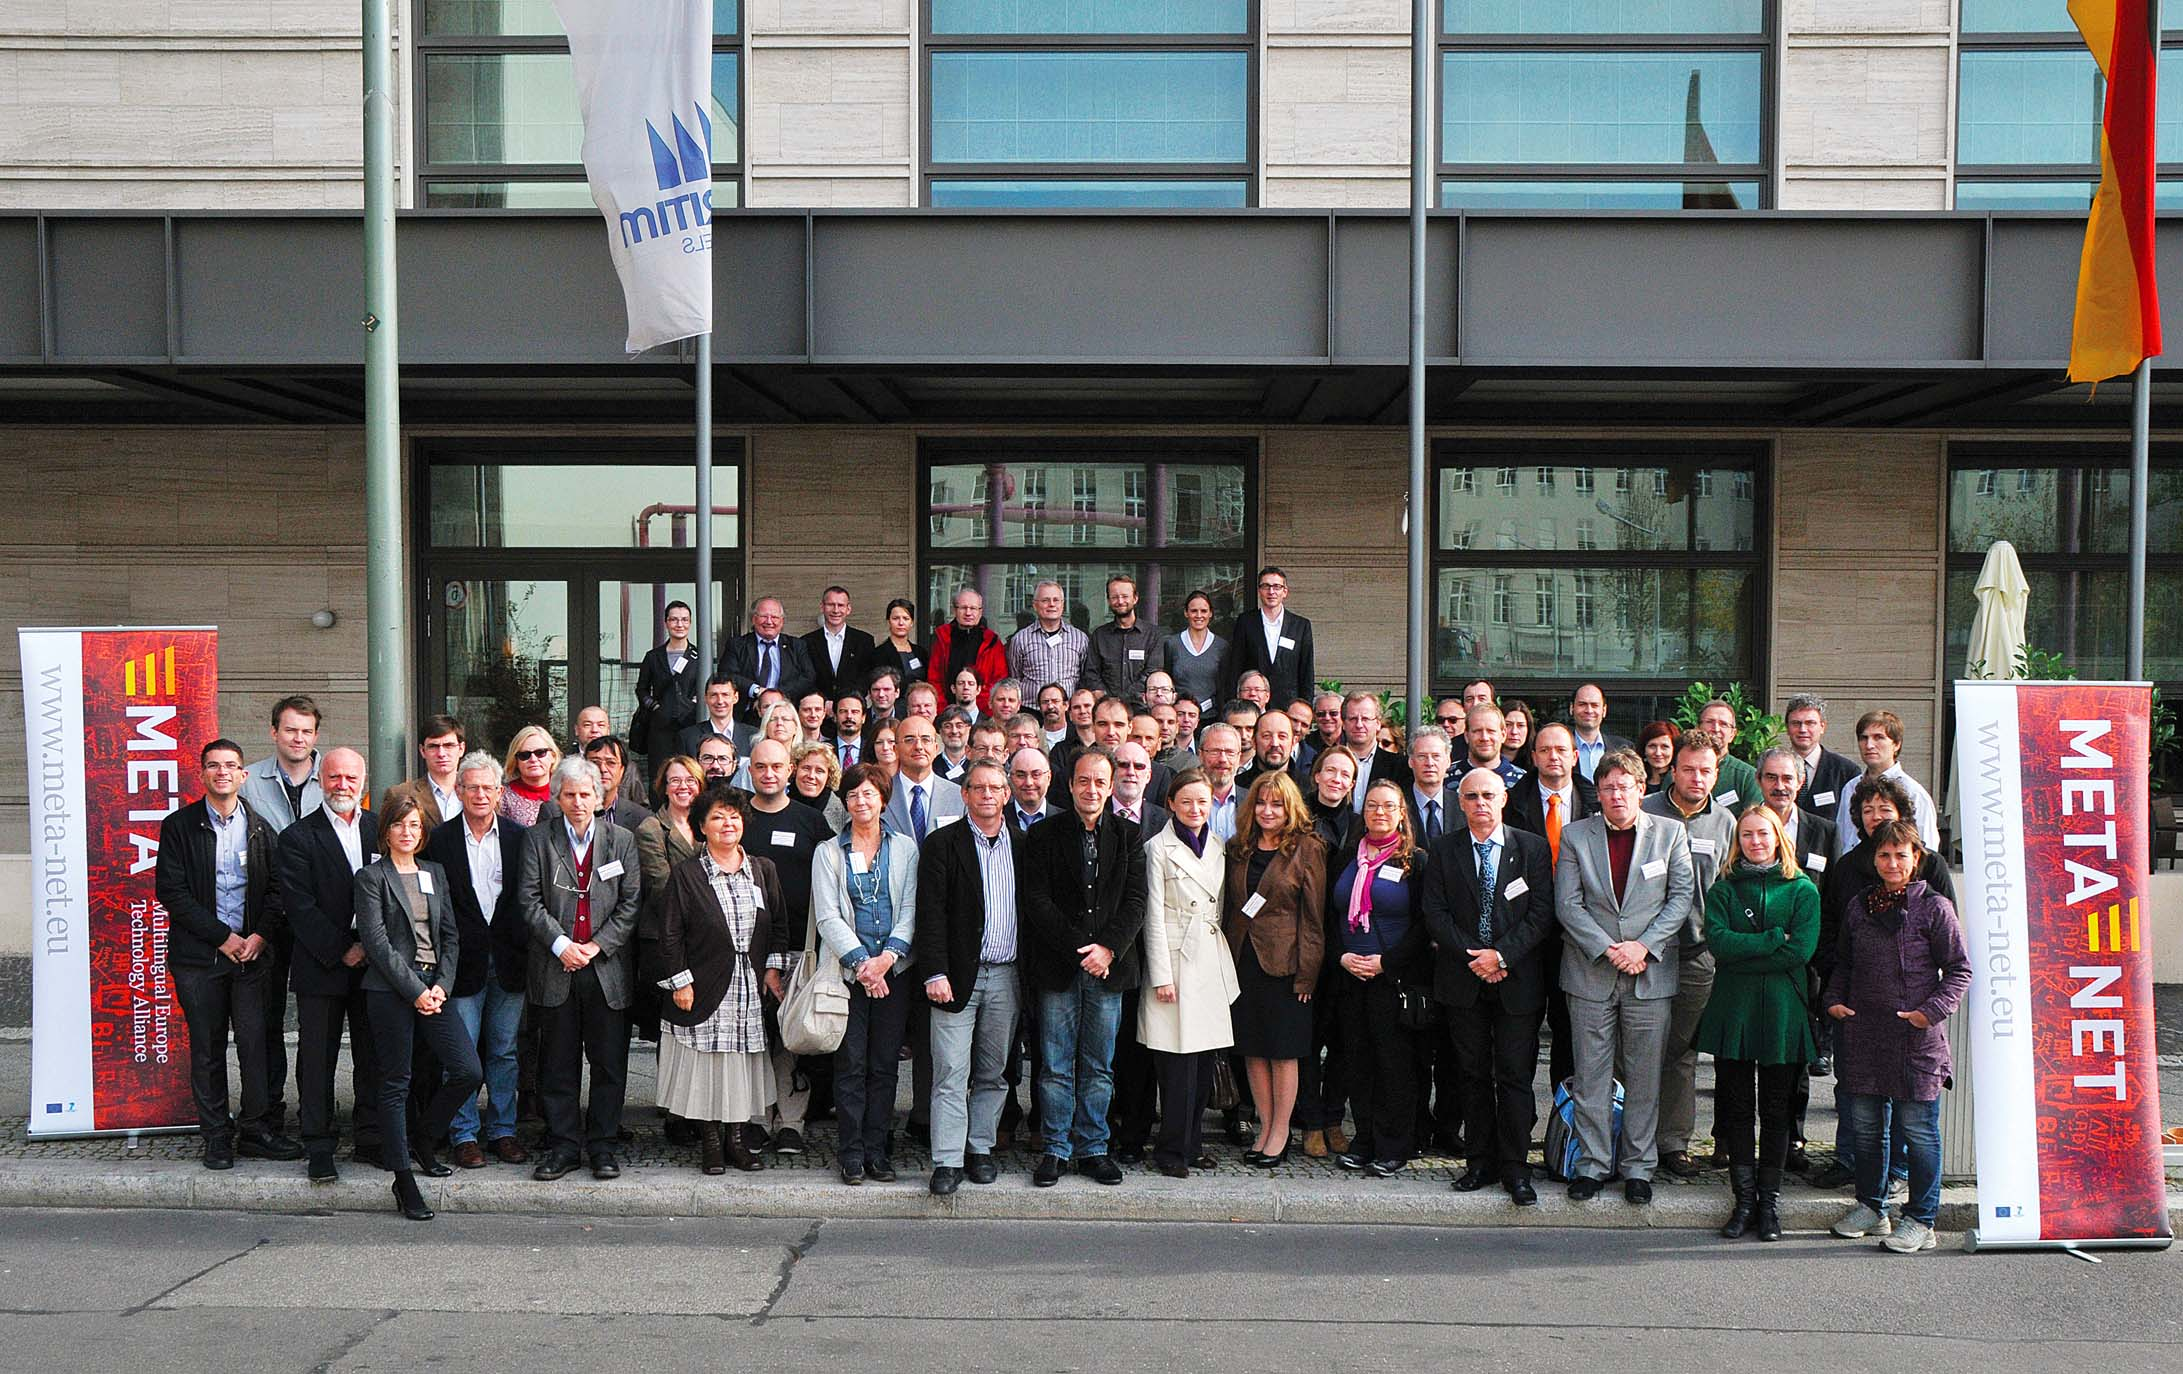
\includegraphics[width=\textwidth]{../_media/meta-net_team_ebook.jpg}
  }{%
    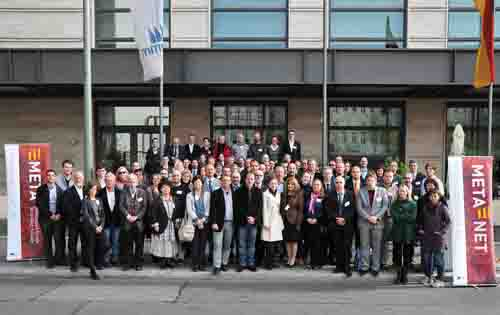
\includegraphics[width=\textwidth]{../_media/meta-net_team.jpg}
  }
  \caption{
Case 100 expertos en tecnoloxías da linguaxe -- representantes dos países e das linguas presentes en META-NET -- analizaron e sacaron conclusións dos resultados e das mensaxes clave da Serie de Libros Brancos nunha reunión META-NET celebrada en Berlín, Alemaña, os días 21 e 22 de outubro de 2011. ---
 \textcolor{grey1}{About 100 language technology experts -- representatives of the countries and languages represented in META-NET -- discussed and finalised the key results and messages of the White Paper Series at a META-NET meeting in Berlin, Germany, on October 21/22, 2011.}}
  \medskip
  \colorrule{grey3}{\textwidth}{1.5pt}
\end{figure*}

\cleardoublepage

\phantomsection
\bsection[Serie de Libros Brancos META-NET -- The META-NET White Paper Series]{Serie de Libros Brancos META-NET --- The META-NET\ \ \ \ \ \ White Paper Series}

\label{whitepaperseries}

\vspace*{-5mm}
\centering
  \setlength{\tabcolsep}{2em}
  \begin{tabularx}{\textwidth}{lllll} \toprule\addlinespace
  %\begin{tabulary}{170mm}{LLL} \toprule
 & Alemán & German & Deutsch\\
 & Búlgaro & Bulgarian & български \\
 & Catalán & Catalan & català\\
 & Checo & Czech & čeština\\
 & Croata & Croatian & hrvatski\\
 & Danés & Danish & dansk\\
 & Eslovaco & Slovak & slovenčina\\
 & Esloveno & Slovene & slovenščina\\
 & Español & Spanish & español\\
 & Estoniano & Estonian & eesti\\
 & Éuscaro & Basque & euskara\\
 & Finlandés & Finnish & suomi\\
 & Francés & French & français\\
 & Galego & Galician & galego\\
 & Grego & Greek & ελληνικά\\
 & Holandés & Dutch & Nederlands\\
 & Húngaro & Hungarian & magyar\\ 
 & Inglés & English & English\\
 & Irlandés & Irish & Gaeilge\\
 & Islandés & Icelandic & íslenska\\
 & Italiano & Italian & italiano\\
 & Letón & Latvian & latviešu valoda\\
 & Lituano & Lithuanian & lietuvių kalba\\
 & Maltés & Maltese & Malti\\
 & Noruegués Bokmål & Norwegian Bokmål & bokmål\\
 & Noruegués Nynorsk & Norwegian Nynorsk & nynorsk\\
 & Polaco & Polish & polski\\
 & Portugués & Portuguese & português\\
 & Romanés & Romanian & română\\
 & Serbio & Serbian & српски\\
 & Sueco & Swedish & svenska\\  \addlinespace \bottomrule
\end{tabularx}
